\documentclass[letterpaper,10pt]{book}
% Change to 10 pt
\usepackage{pdfpages}
\usepackage{morewrites}			% to counteract the no write space problem
\setcounter{tocdepth}{6}

\usepackage[framemethod=TikZ]{mdframed}

\usepackage{fancyhdr}

\usepackage{paralist}
\usepackage{amsmath}
\usepackage{amsfonts}
\usepackage{amssymb}
\usepackage{graphicx}

\usepackage{datetime}
%\usepackage{ulem}

%\usepackage[nottoc]{toobibind}

\usepackage[inline]{enumitem}

% Outer margin at 2.50 is exacty correct to fit the ``corruption alert'' tables
\usepackage[inner=1.0in, outer=2.50in, top=2.54cm,bottom=2.54cm, marginparwidth=2.25in]{geometry}

\usepackage{marginnote}
\usepackage{longtable}
\usepackage{booktabs}
\usepackage{xcolor}

\usepackage{soul}

%%%%%%%%%%%%
\definecolor{ForestGreen}{rgb}{0.00,0.29,0.098}
%%%%%%%%%%%%

\usepackage{marginnote}

\usepackage{imakeidx} 
\usepackage[
	backref=true,
	style=numeric,
%	citestyle=numeric,
	backend=bibtex
	]{biblatex}
\usepackage[driverfallback=hypertex,colorlinks=True]{hyperref}
\usepackage{cleveref}

\makeindex[name=scripture,columnsep=20pt, columnseprule=True,columns=3, title=Scripture References]
\makeindex[name=speaker,columnsep=20pt, columnseprule=True,,columns=2, title=Sermon Creator]
\makeindex[name=series,columnsep=20pt, columnseprule=True,,columns=2, title=Sermon Series]
\makeindex[name=date,columnsep=20pt, columnseprule=True,columns=2, title=Sermon Date]
\makeindex[name=event,columnsep=20pt, columnseprule=True,columns=2, title=Event]
\makeindex[name=topic,columnsep=20pt, columnseprule=True,columns=2, title=Topic]
\makeindex[name=AWIP,columnsep=20pt, columnseprule=True,columns=3, title=All Words in Passage]
\makeindex[name=NWIV,columnsep=20pt, columnseprule=True,columns=3, title=Number of Words in Verse]
\makeindex[name=PNIP,columnsep=20pt, columnseprule=True,columns=3, title=Proper Names in Passage]
\makeindex[name=PEIP,columnsep=20pt, columnseprule=True,columns=2, title=Prophetic Events in Passage]
\makeindex[name=TWPAQ,columnsep=20pt, columnseprule=True,columns=1, title=13-Word Phrases and Quotes]
\makeindex[name=PFTTIS,columnsep=20pt, columnseprule=False,columns=3, title=Phrases found 13 times in scripture]
\makeindex[name=WFTTIS,columnsep=20pt, columnseprule=False,columns=3, title=Words found 13 times in scripture]
\makeindex[name=WFITV,columnsep=20pt, columnseprule=False,columns=3, title=Words found in exactly 13 verses]
\makeindex[name=EVENTS,columnsep=20pt, columnseprule=False,columns=2, title=Sermon Log by Place]
\makeindex[name=QUESTIONS,columnsep=20pt, columnseprule=False,columns=2, title=Bible Questions]
\makeindex[name=DOCTRINES,columnsep=20pt, columnseprule=False,columns=2, title=Doctrines]
\makeindex[name=SONGS,columnsep=20pt, columnseprule=False,columns=1, title=Songs]
\makeindex[name=LOCATION,columnsep=20pt, columnseprule=False,columns= 2, title=Location]
\makeindex[name=FACEBOOK,columnsep=20pt, columnseprule=False,columns=2, title=Facebook]
\makeindex[name=DEVOTIONAL,columnsep=20pt, columnseprule=False,columns=2, title=Devotional Items]
%%%%%%%%%%%%%%%%% EXTRA COLORS
\definecolor{champagne}{rgb}{0.97,0.91,0.81}
\definecolor{bone}{rgb}{0.89,0.85,0.79}
\pagestyle{fancy}
\fancyhf{}
\fancyhead[LE,RO]{\today}
\fancyhead[RE,LO]{Daily Bible Reading}
\fancyhead[CE,CO]{-page \thepage  - }

\fancyfoot[CO,CE]{\leftmark}
%\fancyfoot[LE,RO]{CSCE 692, HW1}

\title{DBR\\
Daily \\ Reads}
\author{Keith Anthony \\
\today }
%+/ffffff +   \pagenumbering{gobble}
\bibliography{Bibliographies/All20220122}

\setlength{\fboxsep}{1.0pt}

\usepackage[utf8]{inputenc}
\usepackage{tikz}

\begin{document}
%%%%%%%%%%%% Tile Page

\begin{titlepage}

\begin{flushright}
\rightskip=-2.5cm
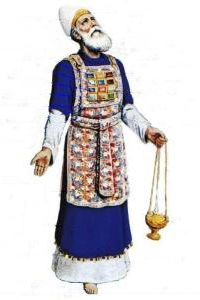
\includegraphics[width=50mm,scale=1.5]{Extras/Melchisedec.jpg}
\vspace{0.4in}  % Create a title for the document and write it in bold font
\LARGE{\textbf{\date}} % Again, do a line break
\linebreak 
% Create a subtitle \large{with Outlines, Statistics, Cross References, and Notes}
\vspace{0.5in}
\begin{flushleft}
\LARGE{Day \#64: Saturday, 5 March 2022  \\}\vspace{0.25in}
\LARGE{Deuteronomy 33-34 Psalm 64 Proverb 5}
\end{flushleft}
\vspace{0.6in}
\bigskip

\normalsize{Xenia, Oh.\\}
\normalsize{created: \today}
\vspace{1.3in}

\end{flushright}
\end{titlepage}

\newpage 
\tableofcontents\hypertarget{TOC}{}
\listoffigures
\listoftables

\hyphenation{A-bim-e-lech bre-thren E-phra-im  Gib-e-o-nites Jer-u-sa-lem through-out Phil-i-stines The-o-phil-us Am-a-le-kites ven-geance Mesh-el-e-mi-ah onan-ism Phar-a-oh thoughts grev-ous-ness Hach-a-liah adul-ter-er Shad-rach}

%%%%%%%%%%%%%%%%% EXTRA COLORS
%%%%%%%%%%%%%%%%% EXTRA COLORS
%%%%%%%%%%%%%%%%% EXTRA COLORS
\definecolor{champagne}{rgb}{0.97,0.91,0.81}
\definecolor{bone}{rgb}{0.89,0.85,0.79}

\definecolor{ForestGreen}{rgb}{0.00,0.29,0.098}
\definecolor{GIVING}{cmyk}{1,0.0,0.72,.1}

\definecolor{MLPE}{cmyk}{1,1,0,.45}
\definecolor{SOCCER}{cmyk}{.77, 0, .42, .49}
\definecolor{PAYBILL}{cmyk}{0,0.83,0.76,0.07}
\definecolor{SERMON}{cmyk}{.14,.9,0,.30} % aka seance \href{http://www.flatuicolorpicker.com/purple-cmyk-color-model/}{seance}
\definecolor{BIBLE}{cmyk}{0,.17,.74,.17}
\definecolor{WORKBLUE}{cmyk}{1, .5, 0, .6}
\definecolor{myOrange}{cmyk}{0, .4, .98, .03}
\definecolor{myTan}{cmyk}{0.0,.07,.17,.10}
\definecolor{myRed}{cmyk}{0,1,1,0}
\definecolor{myWhite}{cmyk}{0,0,0,0}
\definecolor{BLUESoD}{cmyk}{.97,.84,0,.04}
\definecolor{WHITE}{cmyk}{0,0,0,0}
\definecolor{OLDGOLD}{cmyk}{0.05,0.3,1.00,0}
\definecolor{CASTLETON}{cmyk}{1,0,0.31,0.66}
\definecolor{cadmiumgreen}{rgb}{0.0, 0.42, 0.24}
\definecolor{jungle}{rgb}{0.203,0.4882,0.1718}
\definecolor{MYGOLD}{rgb}{1,.84,0}

\definecolor{MYLIGHTGRAY}{rgb}{.85,.85,.85}

\definecolor{codegreen}{rgb}{0,0.6,0}
\definecolor{codegray}{rgb}{0.5,0.5,0.5}
\definecolor{codepurple}{rgb}{0.58,0,0.82}
\definecolor{backcolour}{rgb}{0.95,0.95,0.92}


\mdfdefinestyle{MyFrame}{%
    linecolor=blue,
    outerlinewidth=2pt,
    roundcorner=5pt,
    innertopmargin=\baselineskip,
    innerbottommargin=\baselineskip,
    innerrightmargin=10pt,
    innerleftmargin=10pt,
    backgroundcolor=gray!25!white}


\mdfdefinestyle{MyFrame2}{%
    linecolor=black,
    outerlinewidth=2pt,
    roundcorner=5pt,
    innertopmargin=\baselineskip,
    innerbottommargin=\baselineskip,
    innerrightmargin=10pt,
    innerleftmargin=10pt,
    backgroundcolor=yellow!25!white}


%%%%%
%% for PFTTIS list
%%%%%

%%% And Joseph said unto
\index[PFTTIS]{And Joseph said unto!Genesis!Gen 40:008}
\index[PFTTIS]{And Joseph said unto!Genesis!Gen 40:012}
\index[PFTTIS]{And Joseph said unto!Genesis!Gen 41:025}
\index[PFTTIS]{And Joseph said unto!Genesis!Gen 42:014}
\index[PFTTIS]{And Joseph said unto!Genesis!Gen 42:018}
\index[PFTTIS]{And Joseph said unto!Genesis!Gen 44:015}
\index[PFTTIS]{And Joseph said unto!Genesis!Gen 45:003}
\index[PFTTIS]{And Joseph said unto!Genesis!Gen 45:004}
\index[PFTTIS]{And Joseph said unto!Genesis!Gen 46:031}
\index[PFTTIS]{And Joseph said unto!Genesis!Gen 48:009}
\index[PFTTIS]{And Joseph said unto!Genesis!Gen 48:018}
\index[PFTTIS]{And Joseph said unto!Genesis!Gen 50:019}
\index[PFTTIS]{And Joseph said unto!Genesis!Gen 50:024}


%%% a shadow
\index[PFTTIS]{a shadow!1Chronicles!1Chr 029:15}
\index[PFTTIS]{a shadow!Job!Job 008:09}
\index[PFTTIS]{a shadow!Job!Job 014:02}
\index[PFTTIS]{a shadow!Job!Job 017:07}
\index[PFTTIS]{a shadow!Psalm!Psa 102:011}
\index[PFTTIS]{a shadow!Psalm!Psa 144:004}
\index[PFTTIS]{a shadow!Ecclesiastes!Eccl 006:012}
\index[PFTTIS]{a shadow!Ecclesiastes!Eccl 008:013}
\index[PFTTIS]{a shadow!Isaiah!Isa 04:006}
\index[PFTTIS]{a shadow!Isaiah!Isa 25:004}
\index[PFTTIS]{a shadow!Jonah!Jnh 04:06}
\index[PFTTIS]{a shadow!Colossians!Col 02:017}
\index[PFTTIS]{a shadow!Hebews!Heb 10:001}

%%% blessed is the man
\index[PFTTIS]{blessed is the man!Psalm!Psa 001:001}
\index[PFTTIS]{blessed is the man!Psalm!Psa 032:002}
\index[PFTTIS]{blessed is the man!Psalm!Psa 034:008}
\index[PFTTIS]{blessed is the man!Psalm!Psa 065:004}
\index[PFTTIS]{blessed is the man!Psalm!Psa 084:005}
\index[PFTTIS]{blessed is the man!Psalm!Psa 084:012}
\index[PFTTIS]{blessed is the man!Psalm!Psa 094:012}
\index[PFTTIS]{blessed is the man!Psalm!Psa 112:001}
\index[PFTTIS]{blessed is the man!Proverbs!Pro 008:034}
\index[PFTTIS]{blessed is the man!Isaiah!Isa 056:002}
\index[PFTTIS]{blessed is the man!Jeremiah!Jer 017:007}
\index[PFTTIS]{blessed is the man!Romans!Rom 004:008}
\index[PFTTIS]{blessed is the man!James!Jam 001:012}


%%% carry them
\index[PFTTIS]{carry them!Leviticus!Lev 14:045}
\index[PFTTIS]{carry them!Numbers!Num 11:012}
\index[PFTTIS]{carry them!Joshua!Jsh 04:003}
\index[PFTTIS]{carry them!1Samuel!1Sam 20:040}
\index[PFTTIS]{carry them!1Kings!1Kng 08:046}
\index[PFTTIS]{carry them!2Chronicles!2Chr 06:036}
\index[PFTTIS]{carry them!Ezra!Ezra 05:015}
\index[PFTTIS]{carry them!Isaiah!Isa 40:011}
\index[PFTTIS]{carry them!Isaiah!Isa 41:016}
\index[PFTTIS]{carry them!Isaiah!Isa 57:013}
\index[PFTTIS]{carry them!Jeremiah!Jer 20:004}
\index[PFTTIS]{carry them!Jeremiah!Jer 20:005}
\index[PFTTIS]{carry them!Jeremiah!Jer 43:012}


\index[PFTTIS]{good tidings!2Samuel!2Sam 18:027}
\index[PFTTIS]{good tidings!1Kings!1Ki 01:042}
\index[PFTTIS]{good tidings!2Kings!2Ki 07:009 (2x)}
\index[PFTTIS]{good tidings!Isaiah!Isa 40:009 (2x)}
\index[PFTTIS]{good tidings!Isaiah!Isa 41:007}
\index[PFTTIS]{good tidings!Isaiah!Isa 52:007}
\index[PFTTIS]{good tidings!Isaiah!Isa 61:001}
\index[PFTTIS]{good tidings!Nahum!Nah 01:005}
\index[PFTTIS]{good tidings!Luke!Lk 02:010}
\index[PFTTIS]{good tidings!1Thessalonians!1Thess 03:006}


%%% dead body
\index[PFTTIS]{dead body!Leviticus!Lev 21:011}
\index[PFTTIS]{dead body!Numbers!Num 06:006}
\index[PFTTIS]{dead body!Numbers!Num 09:006}
\index[PFTTIS]{dead body!Numbers!Num 09:007}
\index[PFTTIS]{dead body!Numbers!Num 09:010}
\index[PFTTIS]{dead body!Numbers!Num 09:011}
\index[PFTTIS]{dead body!Numbers!Num 09:013}
\index[PFTTIS]{dead body!Numbers!Num 09:016}
\index[PFTTIS]{dead body!2Kings!2Ki 08:005}
\index[PFTTIS]{dead body!Isaiah!Isa 26:019}
\index[PFTTIS]{dead body!Jeremiah!Jer 26:023}
\index[PFTTIS]{dead body!Jeremiah!Jer 36:030}
\index[PFTTIS]{dead body!Haggai!Hag 02:013}

%%% great sea
\index[PFTTIS]{great sea!Numbers!Num 34:006}
\index[PFTTIS]{great sea!Numbers!Num 34:007}
\index[PFTTIS]{great sea!Joshua!Jos 01:004}
\index[PFTTIS]{great sea!Joshua!Jos 09:001}
\index[PFTTIS]{great sea!Joshua!Jos 15:012}
\index[PFTTIS]{great sea!Joshua!Jos 15:047}
\index[PFTTIS]{great sea!Joshua!Jos 23:004}
\index[PFTTIS]{great sea!Ezekiel!Eze 47:010}
\index[PFTTIS]{great sea!Ezekiel!Eze 47:015}
\index[PFTTIS]{great sea!Ezekiel!Eze 47:019}
\index[PFTTIS]{great sea!Ezekiel!Eze 47:020}
\index[PFTTIS]{great sea!Ezekiel!Eze 48:028}
\index[PFTTIS]{great sea!Daniel!Dan 07:002}


%%% have forsaken me
\index[PFTTIS]{have forsaken me!Judges!Jdg 10:013}
\index[PFTTIS]{have forsaken me!1Samuel!1Sam 08:008}
\index[PFTTIS]{have forsaken me!1Kings!1Ki 11:033}
\index[PFTTIS]{have forsaken me!2Kings!2Ki 22:017}
\index[PFTTIS]{have forsaken me!2Chronicles!2Chr 12:005}
\index[PFTTIS]{have forsaken me!2Chronicles!2Chr 34:025}
\index[PFTTIS]{have forsaken me!Jeremiah!Jer 01:016}
\index[PFTTIS]{have forsaken me!Jeremiah!Jer 02:013}
\index[PFTTIS]{have forsaken me!Jeremiah!Jer 05:007}
\index[PFTTIS]{have forsaken me!Jeremiah!Jer 05:019}
\index[PFTTIS]{have forsaken me!Jeremiah!Jer 16:011 (2x)}
\index[PFTTIS]{have forsaken me!Jeremiah!Jer 19:004}

%%% no king
\index[PFTTIS]{no king!Judges!Jdg 17:06}
\index[PFTTIS]{no king!Judges!Jdg 18:01}
\index[PFTTIS]{no king!Judges!Jdg 19:01}
\index[PFTTIS]{no king!Judges!Jdg 21:25}
\index[PFTTIS]{no king!1Kings!1Ki 22:47}
\index[PFTTIS]{no king!2Kings!2Ki 23:25}
\index[PFTTIS]{no king!Nehemiah!Neh 13:26}
\index[PFTTIS]{no king!Psalms!Psa 033:016}
\index[PFTTIS]{no king!Proverbs!Pro 30:27}
\index[PFTTIS]{no king!Daniel!Dan 02:10}
\index[PFTTIS]{no king!Hosea!Hos 10:03}
\index[PFTTIS]{no king!Micah!Mic 04:09}
\index[PFTTIS]{no king!John!Jhn 19:15}


%%% rebellious house
\index[PFTTIS]{rebellious house!Exodus!Exo 02:005}
\index[PFTTIS]{rebellious house!Exodus!Exo 02:006}
\index[PFTTIS]{rebellious house!Exodus!Exo 02:008}
\index[PFTTIS]{rebellious house!Exodus!Exo 03:009}
\index[PFTTIS]{rebellious house!Exodus!Exo 03:026}
\index[PFTTIS]{rebellious house!Exodus!Exo 03:027}
\index[PFTTIS]{rebellious house!Exodus!Exo 12:002 (2x)}
\index[PFTTIS]{rebellious house!Exodus!Exo 12:003}
\index[PFTTIS]{rebellious house!Exodus!Exo 12:009}
\index[PFTTIS]{rebellious house!Exodus!Exo 12:025}
\index[PFTTIS]{rebellious house!Exodus!Exo 17:012}
\index[PFTTIS]{rebellious house!Exodus!Exo 24:003}

%%% seek him
\index[PFTTIS]{seek him!Deuteronomy!Deu 04:029}\index[PFTTIS]{seek him!1Samuel!1Sam 23:025}
\index[PFTTIS]{seek him!1Chronicles!1Chr 28:009}
\index[PFTTIS]{seek him!2Chronicles!1Chr 15:002}
\index[PFTTIS]{seek him!Ezra!Ezr 08:022}
\index[PFTTIS]{seek him!Psalms!Psa 022:026}
\index[PFTTIS]{seek him!Psalms!Psa 024:006}
\index[PFTTIS]{seek him!Psalms!Psa 119:002}
\index[PFTTIS]{seek him!SoS!SoS 03:002}
\index[PFTTIS]{seek him!SoS!SoS 06:001}
\index[PFTTIS]{seek him!Hosea!Hos 07:010}
\index[PFTTIS]{seek him!Amos!Amo 05:008}
\index[PFTTIS]{seek him!Hebrews!Heb 11:0063}


%%% seek ye
\index[PFTTIS]{seek ye!Isaiah!Isa 34:016}
\index[PFTTIS]{seek ye!Isaiah!Isa 45:019}
\index[PFTTIS]{seek ye!Isaiah!Isa 55:006}
\index[PFTTIS]{seek ye!Amos!Amos 5:004}
\index[PFTTIS]{seek ye!John!John 1:38}
\index[PFTTIS]{seek ye!John!John 18:4}
\index[PFTTIS]{seek ye!John!John 18:7}
\index[PFTTIS]{seek ye!Matthew!Matt 6:33}
\index[PFTTIS]{seek ye!Numbers!Num 16:10}
\index[PFTTIS]{seek ye!Luke!Luke 12:31}
\index[PFTTIS]{seek ye!Luke!Luke 24:5}
\index[PFTTIS]{seek ye!Psalm!Psa 27:8}
\index[PFTTIS]{seek ye!Zephaniah!Zeph 2:3}

%%% the uncircumcised
\index[PFTTIS]{the uncircumcised!Genesis!Gen 17:014}
\index[PFTTIS]{the uncircumcised!Judges!Jdg 14:003}
\index[PFTTIS]{the uncircumcised!Judges!Jdg 15:018}
\index[PFTTIS]{the uncircumcised!2Samuel!2Sam 01:020}
\index[PFTTIS]{the uncircumcised!Isaiah!Isa 02:001}
\index[PFTTIS]{the uncircumcised!Jeremiah!Jer 09:025}
\index[PFTTIS]{the uncircumcised!Ezekiel!Eze 28:010}
\index[PFTTIS]{the uncircumcised!Ezekiel!Eze 31:018}
\index[PFTTIS]{the uncircumcised!Ezekiel!Eze 32:019}
\index[PFTTIS]{the uncircumcised!Ezekiel!Eze 32:027}
\index[PFTTIS]{the uncircumcised!Ezekiel!Eze 32:028}
\index[PFTTIS]{the uncircumcised!Ezekiel!Eze 32:029}
\index[PFTTIS]{the uncircumcised!Ezekiel!Eze 32:032}

%%% worship him
\index[PFTTIS]{worship him!Psalms!Psa 97:007}
\index[PFTTIS]{worship him!Zephaniah!Zeph 02:011}
\index[PFTTIS]{worship him!Matthew!Matt 02:002}
\index[PFTTIS]{worship him!Matthew!Matt 02:008}
\index[PFTTIS]{worship him!John!John 04:023}
\index[PFTTIS]{worship him!John!John 04:024 (2x)} 
\index[PFTTIS]{worship him!Acts!Acts 17:023}
\index[PFTTIS]{worship him!Hebrews!Heb 01:006}
\index[PFTTIS]{worship him!Revelation!Rev 04:010}
\index[PFTTIS]{worship him!Revelation!Rev 13:008}
\index[PFTTIS]{worship him!Revelation!Rev 14:007}
\index[PFTTIS]{worship him!Revelation!Rev 19:010}


%%%%%
%% for PFTTIS list
%%%%%

%%% afflictions
\index[WFTTIS]{afflictions!Psalms!Psa 34:019}
\index[WFTTIS]{afflictions!Psalms!Psa 132:001}
\index[WFTTIS]{afflictions!Acts!Acts 07:010}
\index[WFTTIS]{afflictions!Acts!Acts 20:023}
\index[WFTTIS]{afflictions!2Corinthians!2Cor 06:004}
\index[WFTTIS]{afflictions!Colossians!Col 01:024}
\index[WFTTIS]{afflictions!1Thessalonians!1Thess 03:003}
\index[WFTTIS]{afflictions!2Timothy!2Tim 01:008}
\index[WFTTIS]{afflictions!2Timothy!2Tim 03:011}
\index[WFTTIS]{afflictions!2Timothy!2Tim 04:005}
\index[WFTTIS]{afflictions!Hebrews!Heb 10:032}
\index[WFTTIS]{afflictions!Hebrews!Heb 10:033}
\index[WFTTIS]{afflictions!1Peter!1Pet 05:009}

%%% acsend
\index[WFTTIS]{acsend!Joshua!Jos 06:05}
\index[WFTTIS]{acsend!Psalm!Psa 024:003}
\index[WFTTIS]{acsend!Psalm!Psa 135:007}
\index[WFTTIS]{acsend!Psalm!Psa 139:008}
\index[WFTTIS]{acsend!Isaiah!Isa 14:013}
\index[WFTTIS]{acsend!Isaiah!Isa 14:014}
\index[WFTTIS]{acsend!Jeremiah!Jer 10:013}
\index[WFTTIS]{acsend!Jeremiah!Jer 51:016}
\index[WFTTIS]{acsend!Ezekiel!Eze 38:009}
\index[WFTTIS]{acsend!John!John 06:062}
\index[WFTTIS]{acsend!John!John 20:017}
\index[WFTTIS]{acsend!Romans!Rom 10:006}
\index[WFTTIS]{acsend!Revelation!Rev 17:008}

%%% Assyrian
\index[WFTTIS]{Assyrian!Isaiah!Isa 10:005}
\index[WFTTIS]{Assyrian!Isaiah!Isa 10:024}
\index[WFTTIS]{Assyrian!Isaiah!Isa 14:025}
\index[WFTTIS]{Assyrian!Isaiah!Isa 19:023}
\index[WFTTIS]{Assyrian!Isaiah!Isa 23:013}
\index[WFTTIS]{Assyrian!Isaiah!Isa 30:031}
\index[WFTTIS]{Assyrian!Isaiah!Isa 31:008}
\index[WFTTIS]{Assyrian!Isaiah!Isa 52:004}
\index[WFTTIS]{Assyrian!Ezekiel!Eze 31:003}
\index[WFTTIS]{Assyrian!Hosea!Hos 05:013}
\index[WFTTIS]{Assyrian!Hosea!Hos 11:005}
\index[WFTTIS]{Assyrian!Micah!Hos 05:005}
\index[WFTTIS]{Assyrian!Micah!Hos 05:006}

%%% blot
\index[WFTTIS]{blot!Exodus!Exo 32:032}
\index[WFTTIS]{blot!Exodus!Exo 32:033}
\index[WFTTIS]{blot!Numbers!Num 05:026}
\index[WFTTIS]{blot!Deuteronomy!Deut 09:014}
\index[WFTTIS]{blot!Deuteronomy!Deut 25:019}
\index[WFTTIS]{blot!Deuteronomy!Deut 29:020}
\index[WFTTIS]{blot!2Kings!2Ki 14:027}
\index[WFTTIS]{blot!Job!Job 31:007}
\index[WFTTIS]{blot!Psalms!Psa 51:001}
\index[WFTTIS]{blot!Psalms!Psa 51:009}
\index[WFTTIS]{blot!Proverbs!Pro 09:007}
\index[WFTTIS]{blot!Jeremiah!Jer 18:023}
\index[WFTTIS]{blot!Revelation!Rev 03:005}


%%% chain
\index[WFTTIS]{chain!Genesis!Gen 41:042}
\index[WFTTIS]{chain!1Kings!1Ki 07:017}
\index[WFTTIS]{chain!Psalms!Psa 73:006}
\index[WFTTIS]{chain!SoS!Sos 04:009}
\index[WFTTIS]{chain!Lamentations!Lam 03:007}
\index[WFTTIS]{chain!Ezekiel!Eze 07:023}
\index[WFTTIS]{chain!Ezekiel!Eze 16:011}
\index[WFTTIS]{chain!Daniel!Dan 05:007}
\index[WFTTIS]{chain!Daniel!Dan 05:016}
\index[WFTTIS]{chain!Daniel!Dan 05:029}
\index[WFTTIS]{chain!Acts!Acts 28:020}
\index[WFTTIS]{chain!2Timothy!2Tim 01:016}
\index[WFTTIS]{chain!Revelation!Rev 20:001}


%%% controversy
\index[WFTTIS]{controversy!Deuteronomy!Deu 17:008}
\index[WFTTIS]{controversy!Deuteronomy!Deu 19:017}
\index[WFTTIS]{controversy!Deuteronomy!Deu 21:005}
\index[WFTTIS]{controversy!Deuteronomy!Deu 25:001}
\index[WFTTIS]{controversy!2Samuel!2Sam 15:002}
\index[WFTTIS]{controversy!Isaiah!Isa 34:008}
\index[WFTTIS]{controversy!Jeremiah!Jer 25:031}
\index[WFTTIS]{controversy!Ezekiel!Eze 44:024}
\index[WFTTIS]{controversy!Hosea!Hos 04:001}
\index[WFTTIS]{controversy!Hosea!Hos 12:002}
\index[WFTTIS]{controversy!Micah!Mic 06:002 (2x)}
\index[WFTTIS]{controversy!1Timothy!1Tim 03:016}


%%% Dagon/Dagon's
\index[WFTTIS]{Dagon!Judges!Jdg 16:023}
\index[WFTTIS]{Dagon!1Samuel!1Sam 05:002 (2x)}
\index[WFTTIS]{Dagon!1Samuel!1Sam 05:003 (2x)}
\index[WFTTIS]{Dagon!1Samuel!1Sam 05:004 (3x)}
\index[WFTTIS]{Dagon!1Samuel!1Sam 05:005 (3x)}
\index[WFTTIS]{Dagon!1Samuel!1Sam 05:007}
\index[WFTTIS]{Dagon!1Chronicles!1Chr 10:010}

%%% disobedient
\index[WFTTIS]{disobedient!1Kings!1Ki 13:026}
\index[WFTTIS]{disobedient!Nehemiah!Neh 09:026}
\index[WFTTIS]{disobedient!Luke!Luke 01:017}
\index[WFTTIS]{disobedient!Acts!Acts 26:019}
\index[WFTTIS]{disobedient!Romans!Rom 01:030}
\index[WFTTIS]{disobedient!Romans!Rom 10:021}
\index[WFTTIS]{disobedient!1Timothy!1Tim 01:009}
\index[WFTTIS]{disobedient!2Timothy!2Tim 03:002}
\index[WFTTIS]{disobedient!Titus!Titus 01:016}
\index[WFTTIS]{disobedient!Titus!Titus 03:003}
\index[WFTTIS]{disobedient!1Peter!1Pet 02:007}
\index[WFTTIS]{disobedient!1Peter!1Pet 02:008}
\index[WFTTIS]{disobedient!1Peter!1Pet 03:020}


%%% doubt
\index[WFTTIS]{doubt!Genesis!Gen 37:033}
\index[WFTTIS]{doubt!Deuteronomy!Deu 28:066}
\index[WFTTIS]{doubt!Job!Job 12:002}
\index[WFTTIS]{doubt!Matthew!Matt 14:031}
\index[WFTTIS]{doubt!Matthew!Matt 21:021}
\index[WFTTIS]{doubt!Mark!Mk 11:023}
\index[WFTTIS]{doubt!Luke!Lk 11:020}
\index[WFTTIS]{doubt!John!Jhn 10:024}
\index[WFTTIS]{doubt!Acts!Acts 02:012}
\index[WFTTIS]{doubt!Acts!Acts 28:004}
\index[WFTTIS]{doubt!1Corinthians!1Cor 09:010}
\index[WFTTIS]{doubt!Galatians!Gal 04:020}
\index[WFTTIS]{doubt!1John!1Jhn 02:019}


%%% dungeon
\index[WFTTIS]{dungeon!Genesis!Gen 40:015}
\index[WFTTIS]{dungeon!Genesis!Gen 41:014}
\index[WFTTIS]{dungeon!Exodus!Exo 12:029}
\index[WFTTIS]{dungeon!Jeremiah!Jer 37:016}
\index[WFTTIS]{dungeon!Jeremiah!Jer 38:006 (2x)}
\index[WFTTIS]{dungeon!Jeremiah!Jer 38:007}
\index[WFTTIS]{dungeon!Jeremiah!Jer 38:009}
\index[WFTTIS]{dungeon!Jeremiah!Jer 38:010}
\index[WFTTIS]{dungeon!Jeremiah!Jer 38:011}
\index[WFTTIS]{dungeon!Jeremiah!Jer 38:013}
\index[WFTTIS]{dungeon!Lamentations!Lam 03:053}
\index[WFTTIS]{dungeon!Lamentations!Lam 03:055}


%%% error
\index[WFTTIS]{error!2Samuel!2Sam 06:007}
\index[WFTTIS]{error!Job!Job 19:004}
\index[WFTTIS]{error!Ecclesiastes!Ecc 05:006}
\index[WFTTIS]{error!Ecclesiastes!Ecc 10:005}
\index[WFTTIS]{error!Isaiah!Isa 32:006}
\index[WFTTIS]{error!Daniel!Dan 06:004}
\index[WFTTIS]{error!Matthew!Matt 27:064}
\index[WFTTIS]{error!Romans!Rom 01:027}
\index[WFTTIS]{error!James!Jam 05:020}
\index[WFTTIS]{error!2Peter!2Pet 02:018}
\index[WFTTIS]{error!2Peter!2Pet 03:017}
\index[WFTTIS]{error!1John!1Jn 04:006}
\index[WFTTIS]{error!Jude!Jude 01:011}

%%% fourish
\index[WFTTIS]{fourish!Psalms!Psa 072:007}
\index[WFTTIS]{fourish!Psalms!Psa 072:016}
\index[WFTTIS]{fourish!Psalms!Psa 092:007}
\index[WFTTIS]{fourish!Psalms!Psa 092:012}
\index[WFTTIS]{fourish!Psalms!Psa 092:013}
\index[WFTTIS]{fourish!Psalms!Psa 132:018}
\index[WFTTIS]{fourish!Proverbs!Pro 11:28}
\index[WFTTIS]{fourish!Proverbs!Pro 14:11}
\index[WFTTIS]{fourish!Ecclesiastes!Ecc 12:05}
\index[WFTTIS]{fourish!SongOfSolomon!SOS 07:12}
\index[WFTTIS]{fourish!Isaiah!Isa 17:11}
\index[WFTTIS]{fourish!Isaiah!Isa 66:14}
\index[WFTTIS]{fourish!Ezekiel!Eze 17:24}




%%% giants
\index[WFTTIS]{giants!Genesis!Gen 06:004}
\index[WFTTIS]{giants!Numbers!Num 13:033}
\index[WFTTIS]{giants!Deuteronomy!Deut 02:011}
\index[WFTTIS]{giants!Deuteronomy!Deut 02:021}
\index[WFTTIS]{giants!Deuteronomy!Deut 03:011}
\index[WFTTIS]{giants!Deuteronomy!Deut 03:013}
\index[WFTTIS]{giants!Joshua!Josh 12:004}
\index[WFTTIS]{giants!Joshua!Josh 13:012}
\index[WFTTIS]{giants!Joshua!Josh 15:008}
\index[WFTTIS]{giants!Joshua!Josh 17:015}
\index[WFTTIS]{giants!Joshua!Josh 16:016}

%%% good man
\index[WFTTIS]{good man!2 Samuel!2Sa 18:27}
%(1) Psalms 37:23 [5]
%(1) Psalms 112:5 [2]
%(1) Proverbs 12:2 [2]
%(1) Proverbs 13:22 [2]
%(1) Proverbs 14:14 [14]
%(1) Micah 7:2 [2]
%(1) Matthew 12:35 [2]
%(1) Luke 6:45 [2]
%(1) Luke 23:50 [15]
%(1) John 7:12 [17]
%(1) Acts 11:24 [5]
%(1) Romans 5:7 [14]

%%% Hinnom
\index[WFTTIS]{Hinnom!Joshua!Jsh 15:008}
\index[WFTTIS]{Hinnom!Joshua!Jsh 18:016}
\index[WFTTIS]{Hinnom!2Kings!2Ki 23:010}
\index[WFTTIS]{Hinnom!2Chronicles!2Chr 28:003}
\index[WFTTIS]{Hinnom!2Chronicles!2Chr 33:006}
\index[WFTTIS]{Hinnom!Nehemiah!Neh 11:030}
\index[WFTTIS]{Hinnom!Jeremiah!Jer 07:031}
\index[WFTTIS]{Hinnom!Jeremiah!Jer 07:032}
\index[WFTTIS]{Hinnom!Jeremiah!Jer 19:002}
\index[WFTTIS]{Hinnom!Jeremiah!Jer 19:006}
\index[WFTTIS]{Hinnom!Jeremiah!Jer 32:035}

%%% inclined
\index[WFTTIS]{inclined!Judges!Jdg 09:003}
\index[WFTTIS]{inclined!Psalms!Psa 040:001}
\index[WFTTIS]{inclined!Psalms!Psa 116:002}
\index[WFTTIS]{inclined!Psalms!Psa 119:112}
\index[WFTTIS]{inclined!Proverbs!Pro 05:13}
\index[WFTTIS]{inclined!Jeremiah!Jer 07:24}
\index[WFTTIS]{inclined!Jeremiah!Jer 07:26}
\index[WFTTIS]{inclined!Jeremiah!Jer 11:08}
\index[WFTTIS]{inclined!Jeremiah!Jer 17:23}
\index[WFTTIS]{inclined!Jeremiah!Jer 25:04}
\index[WFTTIS]{inclined!Jeremiah!Jer 34:14}
\index[WFTTIS]{inclined!Jeremiah!Jer 35:15}
\index[WFTTIS]{inclined!Jeremiah!Jer 44:05}


%%% laughed
\index[WFTTIS]{laughed!Genesis!Gen 17:017}
\index[WFTTIS]{laughed!Genesis!Gen 18:012}
\index[WFTTIS]{laughed!Genesis!Gen 18:015}
\index[WFTTIS]{laughed!2Kings!2Ki 19:021}
\index[WFTTIS]{laughed!2Chronicles!2Chr 30:010}
\index[WFTTIS]{laughed!Nehemiah!Neh 02:019}
\index[WFTTIS]{laughed!Job!Job 12:004}
\index[WFTTIS]{laughed!Job!Job 29:024}
\index[WFTTIS]{laughed!Isaiah!Isa 37:022}
\index[WFTTIS]{laughed!Ezekiel!Ezek 23:032}
\index[WFTTIS]{laughed!Matthew!Matt 09:024}
\index[WFTTIS]{laughed!Mark!Mk 05:040}
\index[WFTTIS]{laughed!Luke!Lk 08:053}

%%% liar
\index[WFTTIS]{liar!Job!Job 24:025}
\index[WFTTIS]{liar!Proverbs!Pro 17:004}
\index[WFTTIS]{liar!Proverbs!Pro 19:022}
\index[WFTTIS]{liar!Proverbs!Pro 30:006}
\index[WFTTIS]{liar!Jeremiah!Jer 15:018}
\index[WFTTIS]{liar!John!Jhn 08:044}
\index[WFTTIS]{liar!John!Jhn 08:055}
\index[WFTTIS]{liar!Romans!Rom 03:004}
\index[WFTTIS]{liar!1John!1Jhn 01:010}
\index[WFTTIS]{liar!1John!1Jhn 02:004}
\index[WFTTIS]{liar!1John!1Jhn 02:022}
\index[WFTTIS]{liar!1John!1Jhn 04:020}
\index[WFTTIS]{liar!1John!1Jhn 05:010}

%%% palsy
\index[WFTTIS]{palsy!Matthew!Matt 04:024}
\index[WFTTIS]{palsy!Matthew!Matt 08:006}
\index[WFTTIS]{palsy!Matthew!Matt 09:002}
\index[WFTTIS]{palsy!Matthew!Matt 09:006}
\index[WFTTIS]{palsy!Mark!Mk 02:003}
\index[WFTTIS]{palsy!Mark!Mk 02:004}
\index[WFTTIS]{palsy!Mark!Mk 02:005}
\index[WFTTIS]{palsy!Mark!Mk 02:009}
\index[WFTTIS]{palsy!Mark!Mk 02:010}
\index[WFTTIS]{palsy!Luke!Lk 05:018}
\index[WFTTIS]{palsy!Luke!Lk 05:024}
\index[WFTTIS]{palsy!Acts!Acts 09:033}

%%% Profitable
\index[WFTTIS]{profitable!Job!Job 22:002 (2x)}
\index[WFTTIS]{profitable!Ecclesiastes!Ecc 10:010}
\index[WFTTIS]{profitable!Isaiah!Isa 44:010}
\index[WFTTIS]{profitable!Jeremiah!Jer 13:007}
\index[WFTTIS]{profitable!Matthew!Matt 05:029}
\index[WFTTIS]{profitable!Matthew!Matt 05:030}
\index[WFTTIS]{profitable!Acts!Acts 20:020}
\index[WFTTIS]{profitable!1Timothy!1Tim 04:008}
\index[WFTTIS]{profitable!2Timothy!2Tim 03:016}
\index[WFTTIS]{profitable!2Timothy!2Tim 04:011}
\index[WFTTIS]{profitable!Titus!Titus 03:008}
\index[WFTTIS]{profitable!Philemon!Phlm 01:011}

%%% Rechab
\index[WFTTIS]{Rechab!2Samuel!2Sam 04:002}
\index[WFTTIS]{Rechab!2Samuel!2Sam 04:005}
\index[WFTTIS]{Rechab!2Samuel!2Sam 04:006}
\index[WFTTIS]{Rechab!2Samuel!2Sam 04:009}
\index[WFTTIS]{Rechab!2KIngs!2Ki 10:015}
\index[WFTTIS]{Rechab!2KIngs!2Ki 10:023}
\index[WFTTIS]{Rechab!1Chronicles!1Chr 02:055}
\index[WFTTIS]{Rechab!Nehemiah!Neh 03:014}
\index[WFTTIS]{Rechab!Jeremiah!Jer 35:006}
\index[WFTTIS]{Rechab!Jeremiah!Jer 35:008}
\index[WFTTIS]{Rechab!Jeremiah!Jer 35:014}
\index[WFTTIS]{Rechab!Jeremiah!Jer 35:016}
\index[WFTTIS]{Rechab!Jeremiah!Jer 35:019}

%%% serpents
\index[WFTTIS]{serpents!Exodus!Exo 07:012}
\index[WFTTIS]{serpents!Numbers!Num 21:006}
\index[WFTTIS]{serpents!Numbers!Num 21:007}
\index[WFTTIS]{serpents!Deuteronomy!Deu 08:015}
\index[WFTTIS]{serpents!Deuteronomy!Deu 32:024}
\index[WFTTIS]{serpents!Jeremiah!Jer 08:017}
\index[WFTTIS]{serpents!Matthew!Matt 10:016}
\index[WFTTIS]{serpents!Matthew!Matt 23:033}
\index[WFTTIS]{serpents!Mark!Mk 16:018}
\index[WFTTIS]{serpents!Luke!Lk 10:019}
\index[WFTTIS]{serpents!1Corinthians!1Cor 10:009}
\index[WFTTIS]{serpents!James!Jas 03:007}
\index[WFTTIS]{serpents!Revelation!Rev 09:019}

%%% short
\index[WFTTIS]{short!Numbers!Num 11:023}
\index[WFTTIS]{short!2Kings!2Ki 10:032}
\index[WFTTIS]{short!Job!Job 17:012}
\index[WFTTIS]{short!Job!Job 20:005}
\index[WFTTIS]{short!Psalms!Psa 89:047}
\index[WFTTIS]{short!Romans!Rom 03:023}
\index[WFTTIS]{short!Romans!Rom 09:028  (2x)}
\index[WFTTIS]{short!1Corinthians!1Cor 07:029}
\index[WFTTIS]{short!1Thessalonians!1Thess 02:017}
\index[WFTTIS]{short!Hebrews!Heb 04:001}
\index[WFTTIS]{short!Revelation!Rev 12:012}
\index[WFTTIS]{short!Revelation!Rev 17:010}

%%% smiteth
\index[WFTTIS]{smiteth!Exodus!Exo 21:012}
\index[WFTTIS]{smiteth!Exodus!Exo 21:15}
\index[WFTTIS]{smiteth!Deuteronomy!Dt 25:11}
\index[WFTTIS]{smiteth!Deuteronomy!Dt 27:24}
\index[WFTTIS]{smiteth!Joshua!Jsh 15:16}
\index[WFTTIS]{smiteth!Judges!Jdg 15:16}
\index[WFTTIS]{smiteth!2 Samuel!2Sa 05:08}
\index[WFTTIS]{smiteth!1Chronicles!1Chr 11:06}
\index[WFTTIS]{smiteth!Job!1Chr 26:12}
\index[WFTTIS]{smiteth!Isaiah!Isa 09:13}
\index[WFTTIS]{smiteth!Lamentations!Lam 03:30}
\index[WFTTIS]{smiteth!Ezekiel!Eze 07:09}
\index[WFTTIS]{smiteth!Luke!Lk 06:29}



%%% vanities
\index[WFTTIS]{vanities!Deuteronomy!Deut 21:021}
\index[WFTTIS]{vanities!1Kings!1Ki 16:013}
\index[WFTTIS]{vanities!1Kings!1Ki 16:026}
\index[WFTTIS]{vanities!Psalms!Psa 031:006}
\index[WFTTIS]{vanities!Ecclesiastes!Ecc 01:002 (2x)}
\index[WFTTIS]{vanities!Ecclesiastes!Ecc 05:007}
\index[WFTTIS]{vanities!Ecclesiastes!Ecc 12:008}
\index[WFTTIS]{vanities!Jeremiah!Jer 08:019}
\index[WFTTIS]{vanities!Jeremiah!Jer 10:008}
\index[WFTTIS]{vanities!Jeremiah!Jer 14:022}
\index[WFTTIS]{vanities!Jonah!Jnh 02:008}
\index[WFTTIS]{vanities!Acts!Acts 14:015}



%%%%%
%% for PFTTIS list
%%%%%

%%% worm
\index[WFITV]{worm!Exodus!Exo 16:024}
\index[WFITV]{worm!Job!Job 17:014}
\index[WFITV]{worm!Job!Job 24:029}
\index[WFITV]{worm!Job!Job 25:005 (2x)}
\index[WFITV]{worm!Psalms!Psa 022:006}
\index[WFITV]{worm!Isaiah!Isa 14:011}
\index[WFITV]{worm!Isaiah!Isa 41:014}
\index[WFITV]{worm!Isaiah!Isa 51:008}
\index[WFITV]{worm!Isaiah!Isa 66:024}
\index[WFITV]{worm!Jonah!Jnh 04:007}
\index[WFITV]{worm!Mark!Mk 09:044}
\index[WFITV]{worm!Mark!Mk 09:046}
\index[WFITV]{worm!Mark!Mk 09:048}


%\subsubsection{Title}
%\textbf{Introduction:} Isaiah 46 
%\index[speaker]{Speaker!Isaiah 49 (Title}
%\index[series]{Book (Speaker)!IPassage (Title)}
%\index[date]{2017/07/09!Isaiah 49 (Title)}
%\begin{compactenum}[I.]
%    \item  \textbf{Point} \index[scripture]{Isaiah!IPassage} (IPassage)
%\end{compactenum}




  


%\input{02OT-Exodus/ExodusIntroduction}

%\newpage
%\begin{figure}
%\begin{center}
%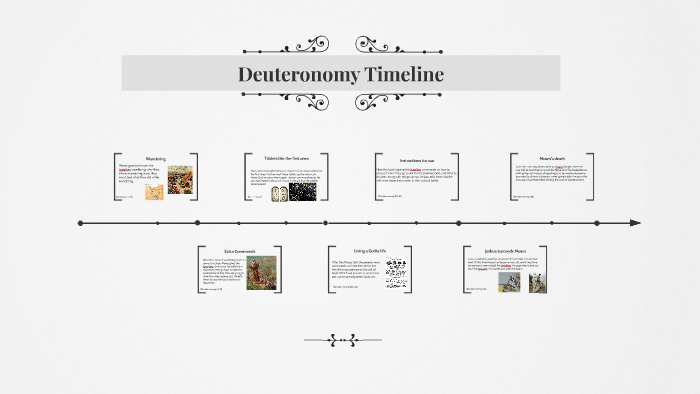
\includegraphics[scale=.7, angle=0]{05OT-Deuteronomy/References/AndrewSmithDeuteronomyTimeline.png}
%\caption[Deuteronomy Timeline by Andrew Smith]{Deuteronomy Timeline by Andrew %Smith}
%\label{fig:Deuteronomy Timeline by Andrew Smith}
%\end{center}
%\end{figure}

\newpage
\begin{figure}
\begin{center}
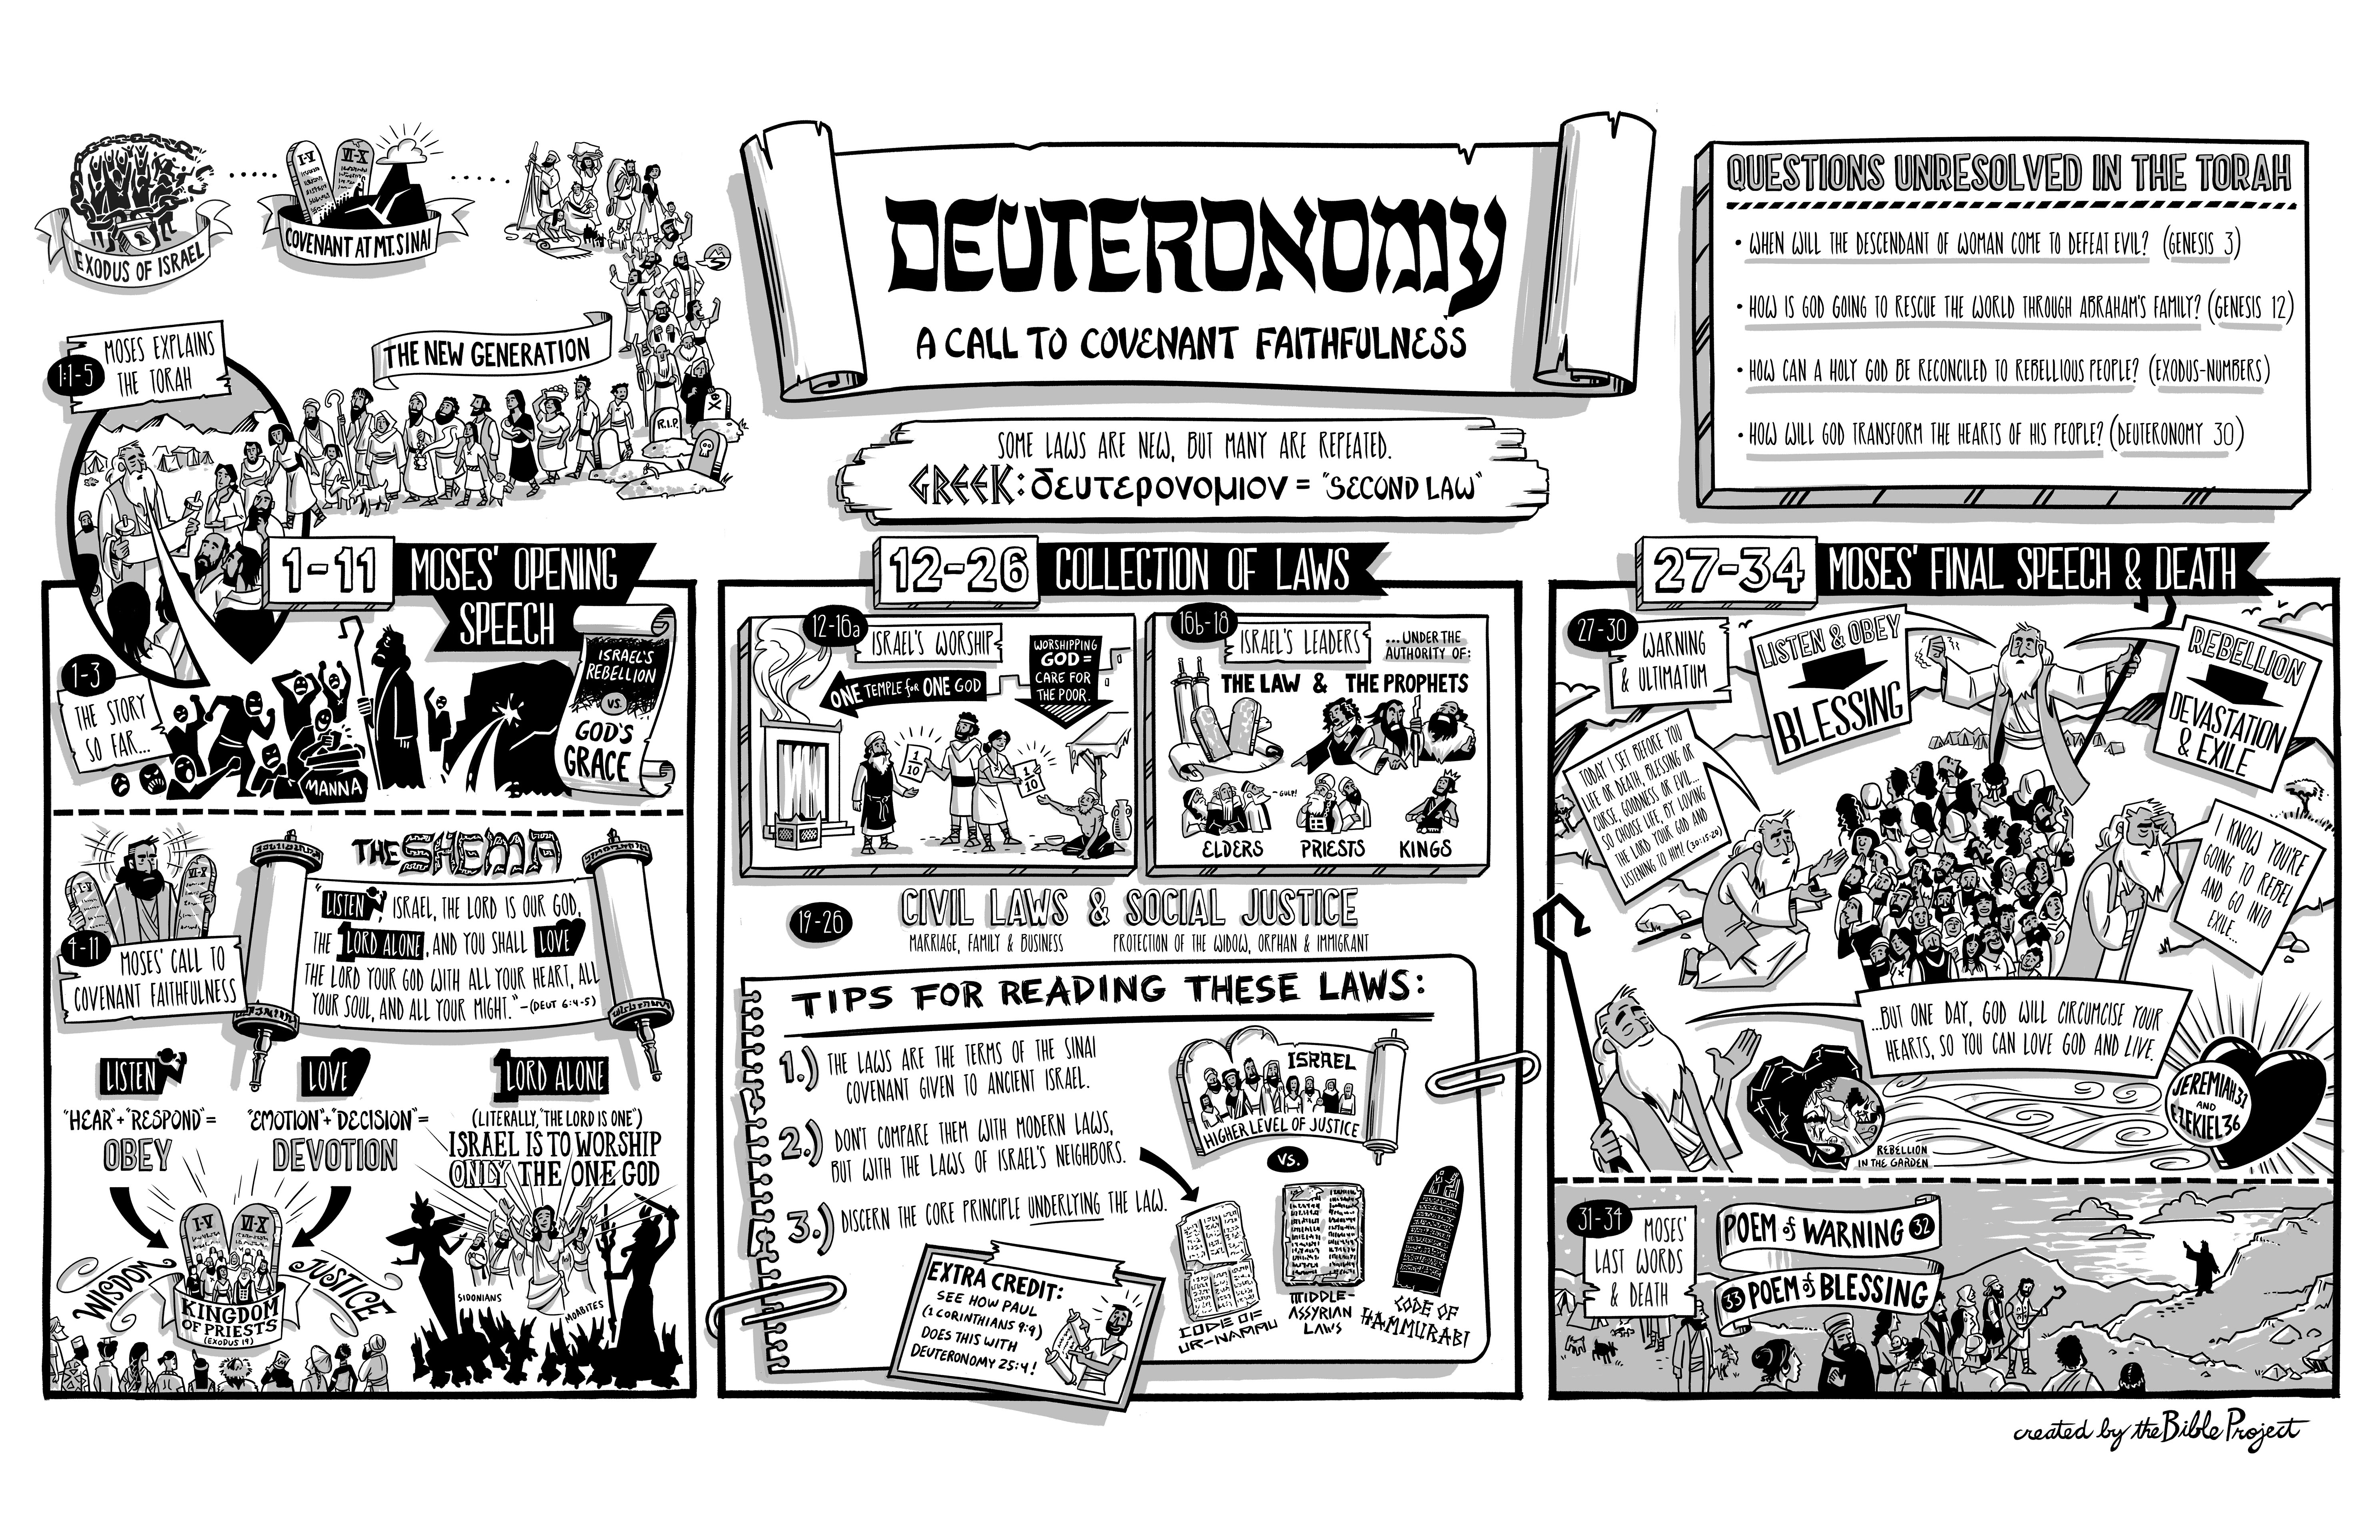
\includegraphics[scale=0.5, angle=90]{05OT-Deuteronomy/References/BibleProject-Deuteronomy.jpg}
\caption[Deuteronomy from the Bible Project]{Deuteronomy from the Bible Project}
\label{fig:Deuteronomy from the Bible Project}
\end{center}
\end{figure}

\newpage
\begin{figure}
\begin{center}
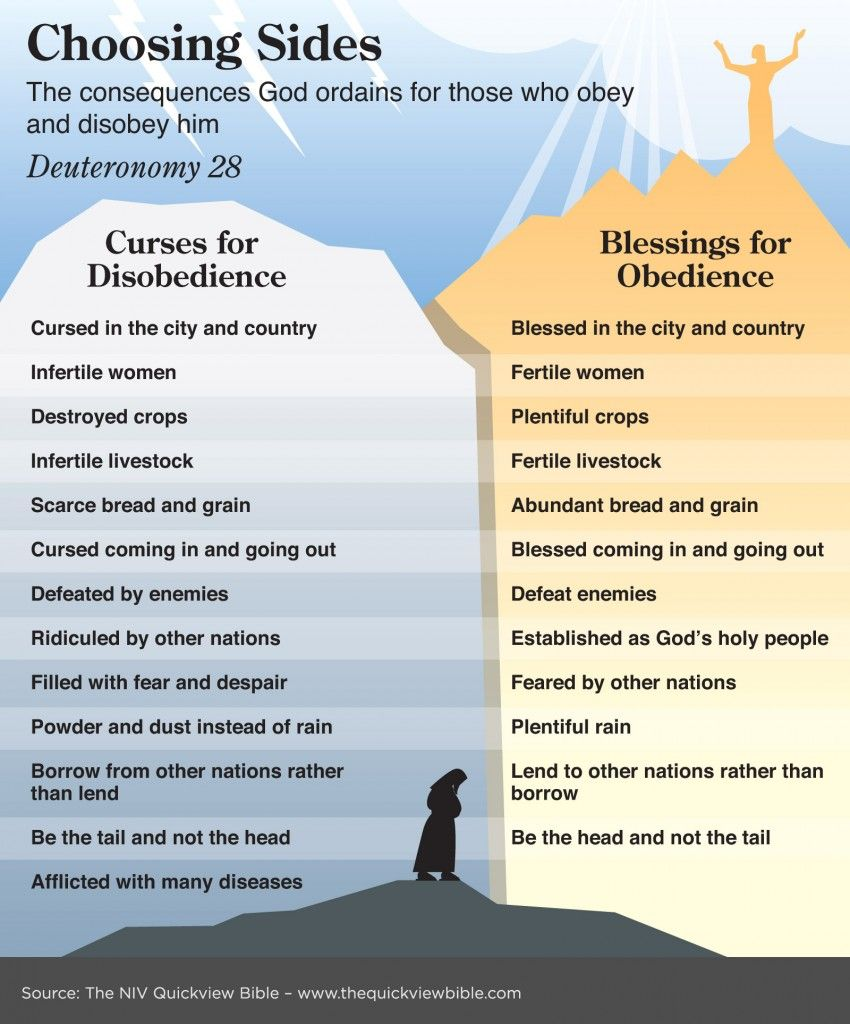
\includegraphics[scale=0.5, angle=0]{05OT-Deuteronomy/References/ChoosingSides.jpeg}
\caption[Choosing Sides]{Choosing Sides}
\label{fig:Choosing Sides}
\end{center}
\end{figure}

\newpage
\begin{figure}
\begin{center}
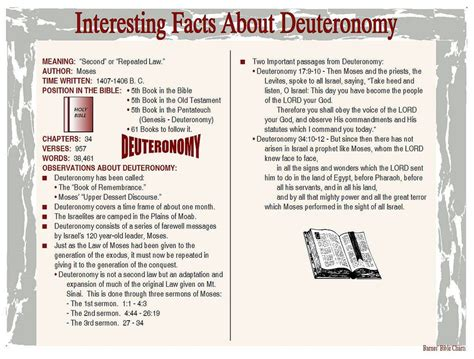
\includegraphics[scale=0.8, angle=90]{05OT-Deuteronomy/References/interestingfactsaboutdeuteronomy.jpeg}
\caption[Interesting Facts About Deuteronomy]{Interesting Facts About Deuteronomy}
\label{fig:Interesting Facts About Deuteronomy}
\end{center}
\end{figure}

\newpage
\begin{figure}
\begin{center}
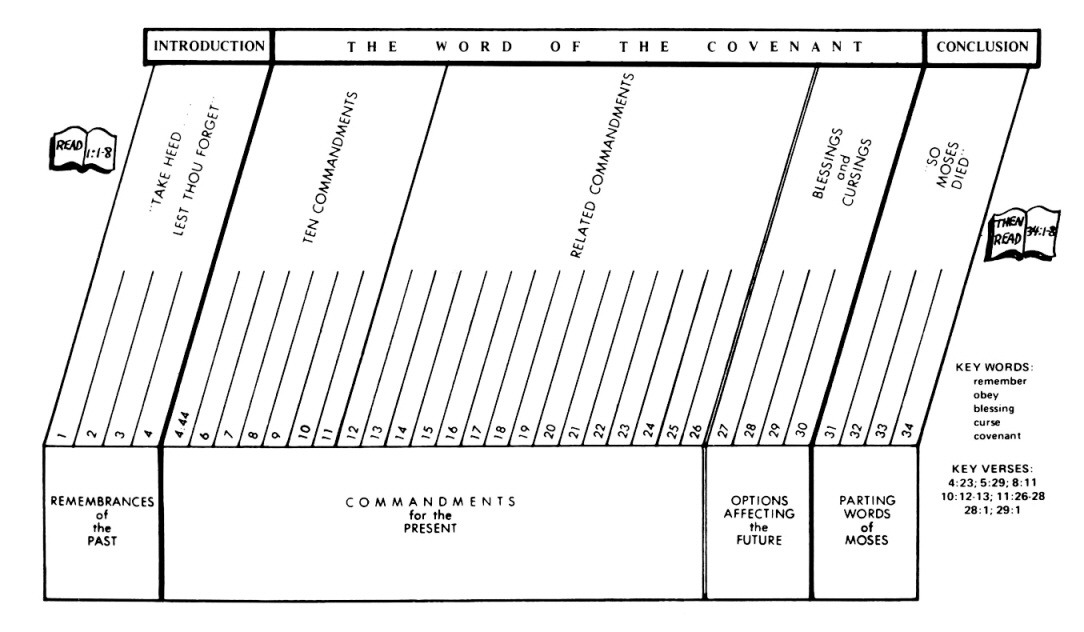
\includegraphics[scale=2.2, angle=90]{05OT-Deuteronomy/References/JensenDeuteronomy.png}
\caption[Deuteronomy by Jensen]{Deuteronomy by Jensen}
\label{fig:Deuteronomy by Jensen}
\end{center}
\end{figure}

\newpage
\begin{figure}
\begin{center}
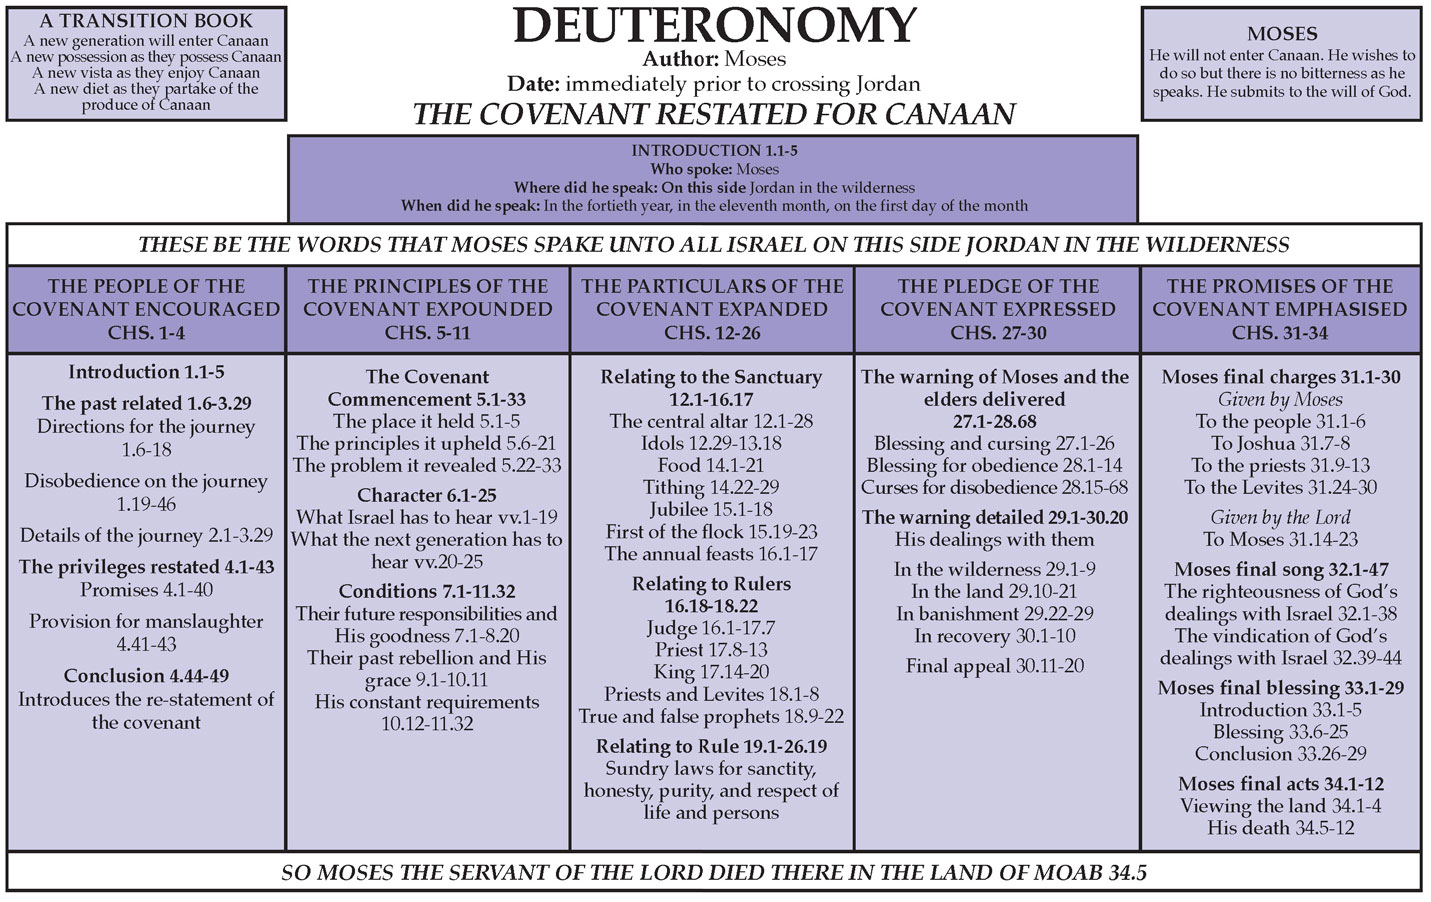
\includegraphics[scale=0.4, angle=90]{05OT-Deuteronomy/References/JohnGrantDeuteronomy.jpg}
\caption[Deuteronomy by John Grant]{Deuteronomy by John Grant}
\label{fig:Deuteronomy by John Grant}
\end{center}
\end{figure}

\newpage
\begin{figure}
\begin{center}
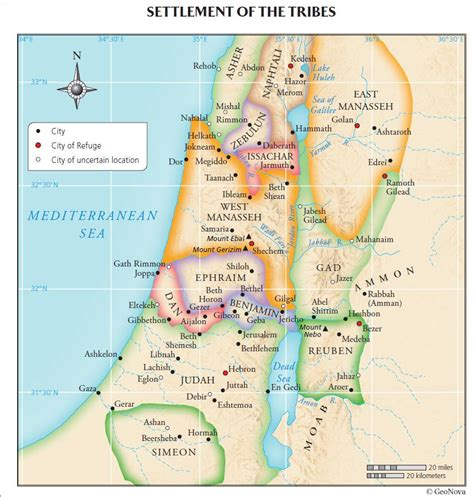
\includegraphics[scale=1, angle=0]{05OT-Deuteronomy/References/SettlementOfTheTribes.jpeg}
\caption[Settlement of the Tribes]{Settlement of the Tribes}
\label{fig:Settlement of the Tribes}
\end{center}
\end{figure}


\newpage
\begin{figure}
\begin{center}
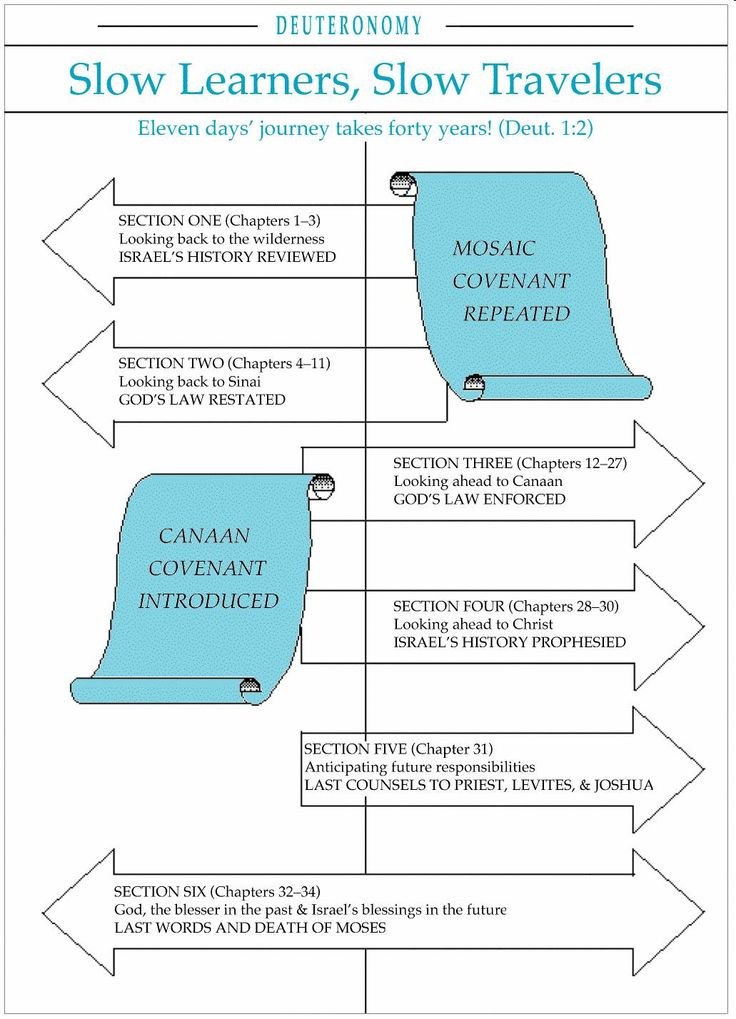
\includegraphics[scale=0.5, angle=0]{05OT-Deuteronomy/References/SlowLearners.jpeg}
\caption[Slow Learners in Deuteronomy]{Slow Learners in Deuteronomy}
\label{fig:Slow Learners in Deuteronomy}
\end{center}
\end{figure}


\newpage
\begin{figure}
\begin{center}
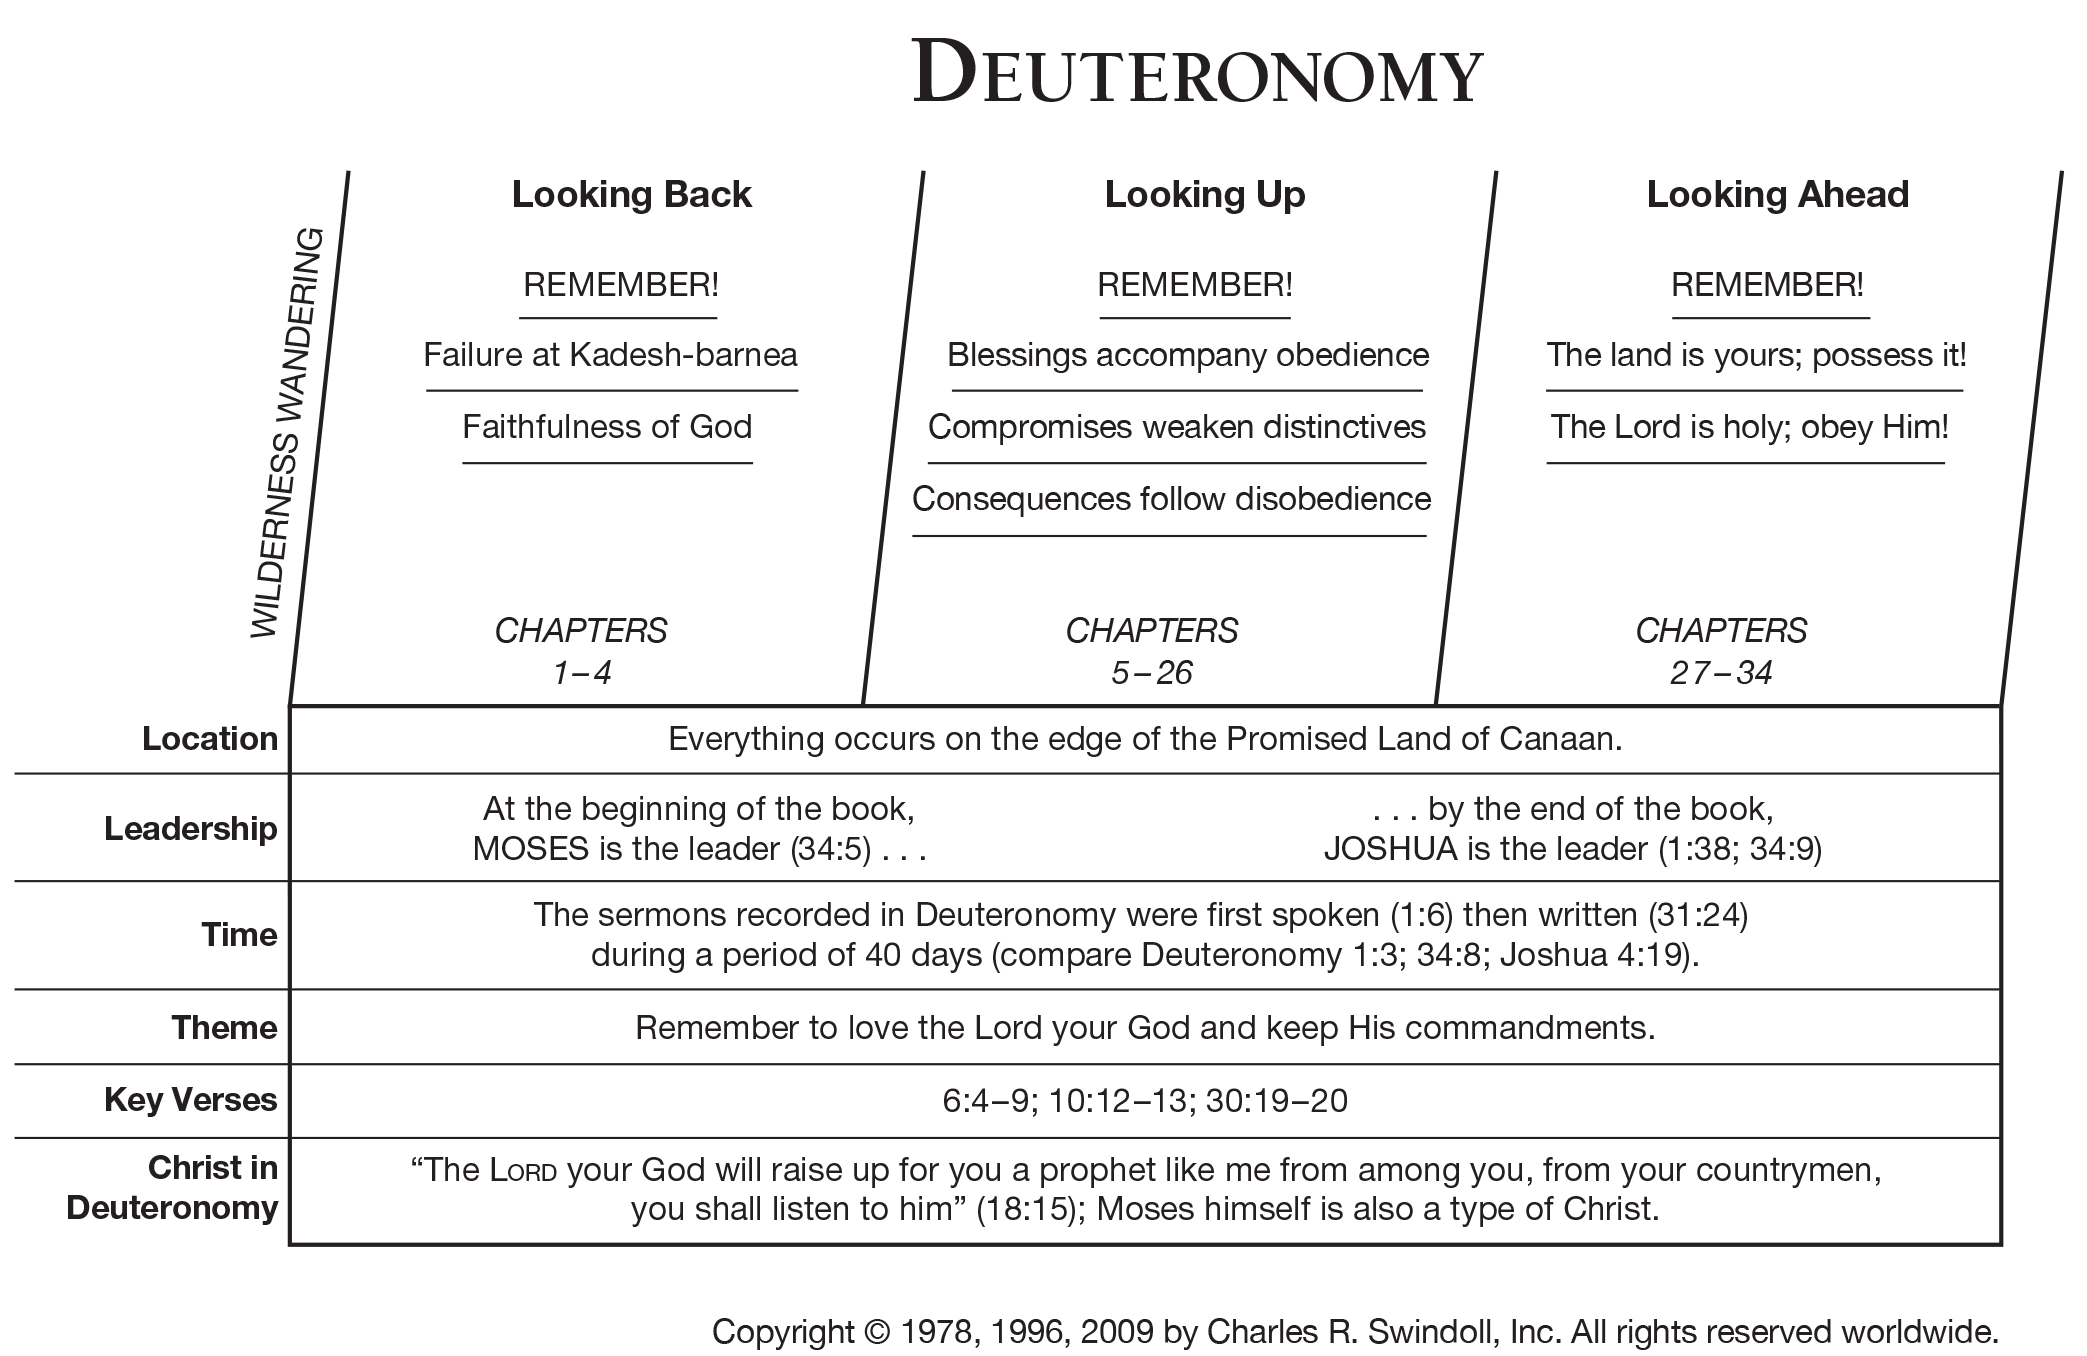
\includegraphics[scale=0.3, angle=90]{05OT-Deuteronomy/References/Swindoll-Deuteronomy.png}
\caption[Deuteronomy by Swindoll]{Deuteronomy by Swindoll}
\label{fig:Deuteronomy by Swindoll}
\end{center}
\end{figure}


\newpage
\begin{figure}
\begin{center}
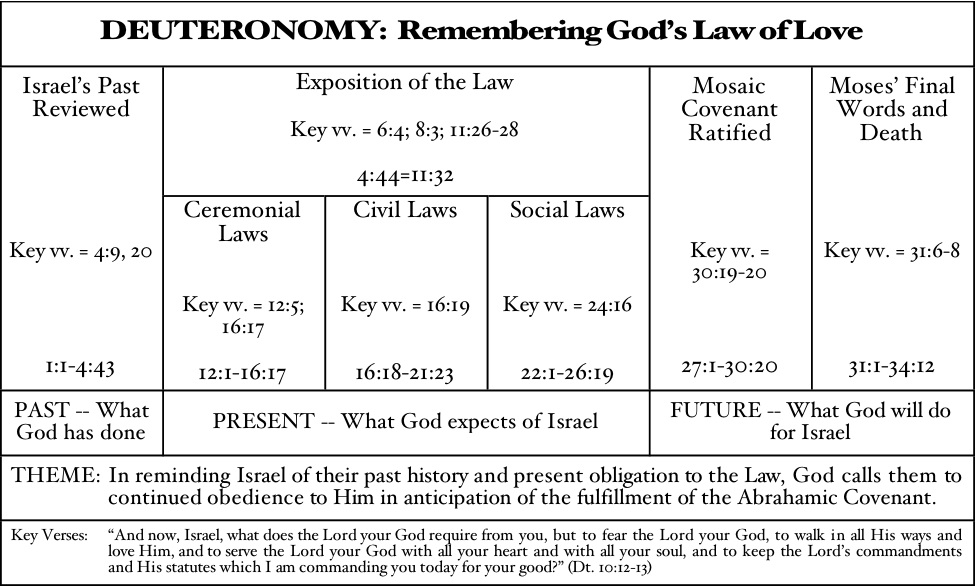
\includegraphics[scale=1, angle=90]{05OT-Deuteronomy/References/WordsOfGrace-Deuteronomy.jpg}
\caption[Deuteronomy from Words of Grace]{Deuteronomy from Words of Grace}
\label{fig:Deuteronomy from Words of Grace}
\end{center}
\end{figure}






\chapter{Deuteronomy 33}






\marginpar{\scriptsize \centering \fcolorbox{bone}{lime}{\textbf{THE LORD RETURNS}}\\ (Deuteronomy 33:1-29) \begin{compactenum}[I.][8]
    \item A \textbf{Mistaken Interpretation} \index[scripture]{Deuteronomy!Deu 33:01--02}(Deu 33:1--2) The verses speak of the second advent and note of the exodus from Egypt
    \item A \textbf{Mighty Return} \index[scripture]{Deuteronomy!Deu 33:02}(Deu 33:2)
    \item The \textbf{Millennial Inheritance} \index[scripture]{Deuteronomy!Deu 33:04}(Deu 33:4)
    \item A \textbf{Massive Gathering} \index[scripture]{Deuteronomy!Deu 33:05}(Deu 33:5)
    \item \textbf{Mercy \fcolorbox{bone}{bone}{for} Reuben} \index[scripture]{Deuteronomy!Deu 33:06}(Deu 33:6) (note 13 words in verse)
    \item A \textbf{Mountain of Gratitude} \index[scripture]{Deuteronomy!Deu 33:19}\index[scripture]{Isaiah!Isaiah 02:02}(Deu 33:19, Isa 2:2) The mountain of the Lord in the Millennium with commemorative sacrifices
    \item A \textbf{Magnificent Guardian} \index[scripture]{Deuteronomy!Deu 33:28}(Deu 33:28) 
\end{compactenum}}






\footnote{\textcolor[cmyk]{0.99998,1,0,0}{\hyperlink{TOC}{Return to end of Table of Contents.}}}\footnote{\href{https://audiobible.com/bible/deuteronomy_33.html}{\textcolor[cmyk]{0.99998,1,0,0}{Deuteronomy 33 Audio}}}\textcolor[cmyk]{0.99998,1,0,0}{And this \emph{is} the blessing, wherewith Moses the man of God blessed the children of Israel before his death.}
[2] \textcolor[cmyk]{0.99998,1,0,0}{And he said, The LORD \fcolorbox{bone}{lime}{came from Sinai}, and rose up from Seir unto them; he shined forth from mount Paran, and he came \fcolorbox{bone}{lime}{with ten thousands of saints}: from his right hand \emph{went} a fiery law \fcolorbox{bone}{bone}{for} them.}
[3] \textcolor[cmyk]{0.99998,1,0,0}{Yea, he loved the people; all his saints \emph{are} in thy hand: and they sat down at thy feet; \emph{every} \emph{one} shall receive of thy words.}
[4] \textcolor[cmyk]{0.99998,1,0,0}{Moses commanded us a law, \emph{even} the \fcolorbox{bone}{lime}{inheritance} of the congregation of Jacob.}
[5] \textcolor[cmyk]{0.99998,1,0,0}{And he was king in Jeshurun, when the heads of the people \emph{and} the tribes of Israel were \fcolorbox{bone}{lime}{gathered} together.}\\
\\
\P \textcolor[cmyk]{0.99998,1,0,0}{\fcolorbox{bone}{lime}{Let Reuben live}, and not die; and let \emph{not} his men be few.}\\
\\
\P \textcolor[cmyk]{0.99998,1,0,0}{And this \emph{is} \emph{the} \emph{blessing} of Judah: and he said, Hear, LORD, the voice of Judah, and bring him unto his people: let his hands be sufficient \fcolorbox{bone}{bone}{for} him; and be thou an help \emph{to} \emph{him} from his enemies.}\\
\\
\P \textcolor[cmyk]{0.99998,1,0,0}{And of Levi he said, \emph{Let} thy Thummim and thy Urim \emph{be} with thy holy one, whom thou didst prove at Massah, \emph{and} \emph{with} whom thou didst strive at the waters of Meribah;}
[9] \textcolor[cmyk]{0.99998,1,0,0}{Who said unto his father and to his mother, I have not seen him; neither did he acknowledge his brethren, nor knew his own children: \fcolorbox{bone}{bone}{for} they have observed thy word, and kept thy covenant.}
[10] \textcolor[cmyk]{0.99998,1,0,0}{They shall teach Jacob thy judgments, and Israel thy law: they shall put incense before thee, and whole burnt sacrifice upon thine altar.}
[11] \textcolor[cmyk]{0.99998,1,0,0}{Bless, LORD, his substance, and accept the work of his hands: smite through the loins of them that rise against him, and of them that hate him, that they rise not again.}\\
\\
\P \textcolor[cmyk]{0.99998,1,0,0}{\emph{And} of Benjamin he said, The beloved of the LORD shall dwell in safety by him; \emph{and} \emph{the} \emph{LORD} shall cover him all the day long, and he shall dwell between his shoulders.}\\
\\
\P \textcolor[cmyk]{0.99998,1,0,0}{And of Joseph he said, Blessed of the LORD \emph{be} his land, \fcolorbox{bone}{bone}{for} the precious things of heaven, \fcolorbox{bone}{bone}{for} the dew, and \fcolorbox{bone}{bone}{for} the deep that coucheth beneath,}
[14] \textcolor[cmyk]{0.99998,1,0,0}{And \fcolorbox{bone}{bone}{for} the precious fruits \emph{brought} \emph{forth} by the sun, and \fcolorbox{bone}{bone}{for} the precious things put forth by the moon,}
[15] \textcolor[cmyk]{0.99998,1,0,0}{And \fcolorbox{bone}{bone}{for} the chief things of the ancient mountains, and \fcolorbox{bone}{bone}{for} the precious things of the lasting hills,}
[16] \textcolor[cmyk]{0.99998,1,0,0}{And \fcolorbox{bone}{bone}{for} the precious things of the earth and fulness thereof, and \emph{for} the good will of him that dwelt in the bush: let \emph{the} \emph{blessing} come upon the head of Joseph, and upon the top of the head of him \emph{that} \emph{was} separated from his brethren.}
[17] \textcolor[cmyk]{0.99998,1,0,0}{His glory \emph{is} \emph{like} the firstling of his bullock, and his horns \emph{are} \emph{like} the horns of unicorns: with them he shall push the people together to the ends of the earth: and they \emph{are} the ten thousands of Ephraim, and they \emph{are} the thousands of Manasseh.}\\
\\
\P \textcolor[cmyk]{0.99998,1,0,0}{And of Zebulun he said, Rejoice, Zebulun, in thy going out; and, Issachar, in thy tents.}
[19] \textcolor[cmyk]{0.99998,1,0,0}{They shall call the people unto the \fcolorbox{bone}{lime}{mountain}; there they shall offer sacrifices of \fcolorbox{bone}{MYGOLD}{righteousness}: \fcolorbox{bone}{bone}{for} they shall suck \emph{of} the abundance of the seas, and \emph{of} treasures hid in the sand.}\\
\\
\P \textcolor[cmyk]{0.99998,1,0,0}{And of Gad he said, Blessed \emph{be} he that enlargeth Gad: he dwelleth as a lion, and teareth the arm with the crown of the head.}
[21] \textcolor[cmyk]{0.99998,1,0,0}{And he provided the first part \fcolorbox{bone}{bone}{for} himself, because there, \emph{in} a portion of the lawgiver, \emph{was} \emph{he} seated; and he came with the heads of the people, he executed the justice of the LORD, and his judgments with Israel.}\\
\\
\P \textcolor[cmyk]{0.99998,1,0,0}{And of Dan he said, Dan \emph{is} a lion's whelp: he shall leap from Bashan.}\\
\\
\P \textcolor[cmyk]{0.99998,1,0,0}{And of Naphtali he said, O Naphtali, satisfied with favour, and full with the blessing of the LORD: possess thou the west and the south.}\\
\\
\P \textcolor[cmyk]{0.99998,1,0,0}{And of Asher he said, \emph{Let} Asher \emph{be} blessed with children; let him be acceptable to his brethren, and let him dip his foot in oil.}
[25] \textcolor[cmyk]{0.99998,1,0,0}{Thy shoes \emph{shall} \emph{be} iron and brass; and as thy days, \emph{so} \emph{shall} thy strength \emph{be}.}\\
\\
\P \textcolor[cmyk]{0.99998,1,0,0}{\emph{There} \emph{is} none like unto the God of Jeshurun, \emph{who} rideth upon the heaven in thy help, and in his excellency on the sky.}
[27] \textcolor[cmyk]{0.99998,1,0,0}{The eternal God \emph{is} \emph{thy} refuge, and underneath \emph{are} the everlasting arms: and he shall thrust out the enemy from before thee; and shall say, Destroy \emph{them}.}
[28] \textcolor[cmyk]{0.99998,1,0,0}{Israel then shall \fcolorbox{bone}{lime}{dwell in safety alone}: the fountain of Jacob \emph{shall} \emph{be} upon a land of corn and wine; also his heavens shall drop down dew.}
[29] \textcolor[cmyk]{0.99998,1,0,0}{Happy \emph{art} thou, O Israel: who \emph{is} like unto thee, O people saved by the LORD, the shield of thy help, and who \emph{is} the sword of thy excellency! and thine enemies shall be found liars unto thee; and thou shalt tread upon their high places.}


\index[NWIV]{19!Deuteronomu!Deu 33:1}\index[AWIP]{And!Deuteronomu!Deu 33:1}\index[AWIP]{this!Deuteronomu!Deu 33:1}\index[AWIP]{\emph{is}!Deuteronomu!Deu 33:1}\index[AWIP]{the!Deuteronomu!Deu 33:1}\index[AWIP]{the!Deuteronomu!Deu 33:1 (2)}\index[AWIP]{the!Deuteronomu!Deu 33:1 (3)}\index[AWIP]{blessing!Deuteronomu!Deu 33:1}\index[AWIP]{wherewith!Deuteronomu!Deu 33:1}\index[AWIP]{Moses!Deuteronomu!Deu 33:1}\index[AWIP]{man!Deuteronomu!Deu 33:1}\index[AWIP]{of!Deuteronomu!Deu 33:1}\index[AWIP]{of!Deuteronomu!Deu 33:1 (2)}\index[AWIP]{God!Deuteronomu!Deu 33:1}\index[AWIP]{blessed!Deuteronomu!Deu 33:1}\index[AWIP]{children!Deuteronomu!Deu 33:1}\index[AWIP]{Israel!Deuteronomu!Deu 33:1}\index[AWIP]{before!Deuteronomu!Deu 33:1}\index[AWIP]{his!Deuteronomu!Deu 33:1}\index[AWIP]{death!Deuteronomu!Deu 33:1}\index[AWIP]{\emph{is}!Deuteronomu!Deu 33:1}

\index[NWIV]{39!Deuteronomu!Deu 33:2}\index[AWIP]{And!Deuteronomu!Deu 33:2}\index[AWIP]{he!Deuteronomu!Deu 33:2}\index[AWIP]{he!Deuteronomu!Deu 33:2 (2)}\index[AWIP]{he!Deuteronomu!Deu 33:2 (3)}\index[AWIP]{said!Deuteronomu!Deu 33:2}\index[AWIP]{The!Deuteronomu!Deu 33:2}\index[AWIP]{LORD!Deuteronomu!Deu 33:2}\index[AWIP]{came!Deuteronomu!Deu 33:2}\index[AWIP]{came!Deuteronomu!Deu 33:2 (2)}\index[AWIP]{from!Deuteronomu!Deu 33:2}\index[AWIP]{from!Deuteronomu!Deu 33:2 (2)}\index[AWIP]{from!Deuteronomu!Deu 33:2 (3)}\index[AWIP]{from!Deuteronomu!Deu 33:2 (4)}\index[AWIP]{Sinai!Deuteronomu!Deu 33:2}\index[AWIP]{and!Deuteronomu!Deu 33:2}\index[AWIP]{and!Deuteronomu!Deu 33:2 (2)}\index[AWIP]{rose!Deuteronomu!Deu 33:2}\index[AWIP]{up!Deuteronomu!Deu 33:2}\index[AWIP]{Seir!Deuteronomu!Deu 33:2}\index[AWIP]{unto!Deuteronomu!Deu 33:2}\index[AWIP]{them!Deuteronomu!Deu 33:2}\index[AWIP]{them!Deuteronomu!Deu 33:2 (2)}\index[AWIP]{shined!Deuteronomu!Deu 33:2}\index[AWIP]{forth!Deuteronomu!Deu 33:2}\index[AWIP]{mount!Deuteronomu!Deu 33:2}\index[AWIP]{Paran!Deuteronomu!Deu 33:2}\index[AWIP]{with!Deuteronomu!Deu 33:2}\index[AWIP]{ten!Deuteronomu!Deu 33:2}\index[AWIP]{thousands!Deuteronomu!Deu 33:2}\index[AWIP]{of!Deuteronomu!Deu 33:2}\index[AWIP]{saints!Deuteronomu!Deu 33:2}\index[AWIP]{his!Deuteronomu!Deu 33:2}\index[AWIP]{right!Deuteronomu!Deu 33:2}\index[AWIP]{hand!Deuteronomu!Deu 33:2}\index[AWIP]{\emph{went}!Deuteronomu!Deu 33:2}\index[AWIP]{a!Deuteronomu!Deu 33:2}\index[AWIP]{fiery!Deuteronomu!Deu 33:2}\index[AWIP]{law!Deuteronomu!Deu 33:2}\index[AWIP]{for!Deuteronomu!Deu 33:2}\index[AWIP]{\emph{went}!Deuteronomu!Deu 33:2}

\index[NWIV]{26!Deuteronomu!Deu 33:3}\index[AWIP]{Yea!Deuteronomu!Deu 33:3}\index[AWIP]{he!Deuteronomu!Deu 33:3}\index[AWIP]{loved!Deuteronomu!Deu 33:3}\index[AWIP]{the!Deuteronomu!Deu 33:3}\index[AWIP]{people!Deuteronomu!Deu 33:3}\index[AWIP]{all!Deuteronomu!Deu 33:3}\index[AWIP]{his!Deuteronomu!Deu 33:3}\index[AWIP]{saints!Deuteronomu!Deu 33:3}\index[AWIP]{\emph{are}!Deuteronomu!Deu 33:3}\index[AWIP]{in!Deuteronomu!Deu 33:3}\index[AWIP]{thy!Deuteronomu!Deu 33:3}\index[AWIP]{thy!Deuteronomu!Deu 33:3 (2)}\index[AWIP]{thy!Deuteronomu!Deu 33:3 (3)}\index[AWIP]{hand!Deuteronomu!Deu 33:3}\index[AWIP]{and!Deuteronomu!Deu 33:3}\index[AWIP]{they!Deuteronomu!Deu 33:3}\index[AWIP]{sat!Deuteronomu!Deu 33:3}\index[AWIP]{down!Deuteronomu!Deu 33:3}\index[AWIP]{at!Deuteronomu!Deu 33:3}\index[AWIP]{feet!Deuteronomu!Deu 33:3}\index[AWIP]{\emph{every}!Deuteronomu!Deu 33:3}\index[AWIP]{\emph{one}!Deuteronomu!Deu 33:3}\index[AWIP]{shall!Deuteronomu!Deu 33:3}\index[AWIP]{receive!Deuteronomu!Deu 33:3}\index[AWIP]{of!Deuteronomu!Deu 33:3}\index[AWIP]{words!Deuteronomu!Deu 33:3}\index[AWIP]{\emph{are}!Deuteronomu!Deu 33:3}\index[AWIP]{\emph{every}!Deuteronomu!Deu 33:3}\index[AWIP]{\emph{one}!Deuteronomu!Deu 33:3}

\index[NWIV]{13!Deuteronomu!Deu 33:4}\index[AWIP]{Moses!Deuteronomu!Deu 33:4}\index[AWIP]{commanded!Deuteronomu!Deu 33:4}\index[AWIP]{us!Deuteronomu!Deu 33:4}\index[AWIP]{a!Deuteronomu!Deu 33:4}\index[AWIP]{law!Deuteronomu!Deu 33:4}\index[AWIP]{\emph{even}!Deuteronomu!Deu 33:4}\index[AWIP]{the!Deuteronomu!Deu 33:4}\index[AWIP]{the!Deuteronomu!Deu 33:4 (2)}\index[AWIP]{inheritance!Deuteronomu!Deu 33:4}\index[AWIP]{of!Deuteronomu!Deu 33:4}\index[AWIP]{of!Deuteronomu!Deu 33:4 (2)}\index[AWIP]{congregation!Deuteronomu!Deu 33:4}\index[AWIP]{Jacob!Deuteronomu!Deu 33:4}\index[AWIP]{\emph{even}!Deuteronomu!Deu 33:4}

\index[NWIV]{20!Deuteronomu!Deu 33:5}\index[AWIP]{And!Deuteronomu!Deu 33:5}\index[AWIP]{he!Deuteronomu!Deu 33:5}\index[AWIP]{was!Deuteronomu!Deu 33:5}\index[AWIP]{king!Deuteronomu!Deu 33:5}\index[AWIP]{in!Deuteronomu!Deu 33:5}\index[AWIP]{Jeshurun!Deuteronomu!Deu 33:5}\index[AWIP]{when!Deuteronomu!Deu 33:5}\index[AWIP]{the!Deuteronomu!Deu 33:5}\index[AWIP]{the!Deuteronomu!Deu 33:5 (2)}\index[AWIP]{the!Deuteronomu!Deu 33:5 (3)}\index[AWIP]{heads!Deuteronomu!Deu 33:5}\index[AWIP]{of!Deuteronomu!Deu 33:5}\index[AWIP]{of!Deuteronomu!Deu 33:5 (2)}\index[AWIP]{people!Deuteronomu!Deu 33:5}\index[AWIP]{\emph{and}!Deuteronomu!Deu 33:5}\index[AWIP]{tribes!Deuteronomu!Deu 33:5}\index[AWIP]{Israel!Deuteronomu!Deu 33:5}\index[AWIP]{were!Deuteronomu!Deu 33:5}\index[AWIP]{gathered!Deuteronomu!Deu 33:5}\index[AWIP]{together!Deuteronomu!Deu 33:5}\index[AWIP]{\emph{and}!Deuteronomu!Deu 33:5}

\index[NWIV]{13!Deuteronomu!Deu 33:6}\index[AWIP]{Let!Deuteronomu!Deu 33:6}\index[AWIP]{Reuben!Deuteronomu!Deu 33:6}\index[AWIP]{live!Deuteronomu!Deu 33:6}\index[AWIP]{and!Deuteronomu!Deu 33:6}\index[AWIP]{and!Deuteronomu!Deu 33:6 (2)}\index[AWIP]{not!Deuteronomu!Deu 33:6}\index[AWIP]{die!Deuteronomu!Deu 33:6}\index[AWIP]{let!Deuteronomu!Deu 33:6}\index[AWIP]{\emph{not}!Deuteronomu!Deu 33:6}\index[AWIP]{his!Deuteronomu!Deu 33:6}\index[AWIP]{men!Deuteronomu!Deu 33:6}\index[AWIP]{be!Deuteronomu!Deu 33:6}\index[AWIP]{few!Deuteronomu!Deu 33:6}\index[AWIP]{\emph{not}!Deuteronomu!Deu 33:6}

\index[NWIV]{39!Deuteronomu!Deu 33:7}\index[AWIP]{And!Deuteronomu!Deu 33:7}\index[AWIP]{this!Deuteronomu!Deu 33:7}\index[AWIP]{\emph{is}!Deuteronomu!Deu 33:7}\index[AWIP]{\emph{the}!Deuteronomu!Deu 33:7}\index[AWIP]{\emph{blessing}!Deuteronomu!Deu 33:7}\index[AWIP]{of!Deuteronomu!Deu 33:7}\index[AWIP]{of!Deuteronomu!Deu 33:7 (2)}\index[AWIP]{Judah!Deuteronomu!Deu 33:7}\index[AWIP]{Judah!Deuteronomu!Deu 33:7 (2)}\index[AWIP]{and!Deuteronomu!Deu 33:7}\index[AWIP]{and!Deuteronomu!Deu 33:7 (2)}\index[AWIP]{and!Deuteronomu!Deu 33:7 (3)}\index[AWIP]{he!Deuteronomu!Deu 33:7}\index[AWIP]{said!Deuteronomu!Deu 33:7}\index[AWIP]{Hear!Deuteronomu!Deu 33:7}\index[AWIP]{LORD!Deuteronomu!Deu 33:7}\index[AWIP]{the!Deuteronomu!Deu 33:7}\index[AWIP]{voice!Deuteronomu!Deu 33:7}\index[AWIP]{bring!Deuteronomu!Deu 33:7}\index[AWIP]{him!Deuteronomu!Deu 33:7}\index[AWIP]{him!Deuteronomu!Deu 33:7 (2)}\index[AWIP]{unto!Deuteronomu!Deu 33:7}\index[AWIP]{his!Deuteronomu!Deu 33:7}\index[AWIP]{his!Deuteronomu!Deu 33:7 (2)}\index[AWIP]{his!Deuteronomu!Deu 33:7 (3)}\index[AWIP]{people!Deuteronomu!Deu 33:7}\index[AWIP]{let!Deuteronomu!Deu 33:7}\index[AWIP]{hands!Deuteronomu!Deu 33:7}\index[AWIP]{be!Deuteronomu!Deu 33:7}\index[AWIP]{be!Deuteronomu!Deu 33:7 (2)}\index[AWIP]{sufficient!Deuteronomu!Deu 33:7}\index[AWIP]{for!Deuteronomu!Deu 33:7}\index[AWIP]{thou!Deuteronomu!Deu 33:7}\index[AWIP]{an!Deuteronomu!Deu 33:7}\index[AWIP]{help!Deuteronomu!Deu 33:7}\index[AWIP]{\emph{to}!Deuteronomu!Deu 33:7}\index[AWIP]{\emph{him}!Deuteronomu!Deu 33:7}\index[AWIP]{from!Deuteronomu!Deu 33:7}\index[AWIP]{enemies!Deuteronomu!Deu 33:7}\index[AWIP]{\emph{is}!Deuteronomu!Deu 33:7}\index[AWIP]{\emph{the}!Deuteronomu!Deu 33:7}\index[AWIP]{\emph{blessing}!Deuteronomu!Deu 33:7}\index[AWIP]{\emph{to}!Deuteronomu!Deu 33:7}\index[AWIP]{\emph{him}!Deuteronomu!Deu 33:7}

\index[NWIV]{33!Deuteronomu!Deu 33:8}\index[AWIP]{And!Deuteronomu!Deu 33:8}\index[AWIP]{of!Deuteronomu!Deu 33:8}\index[AWIP]{of!Deuteronomu!Deu 33:8 (2)}\index[AWIP]{Levi!Deuteronomu!Deu 33:8}\index[AWIP]{he!Deuteronomu!Deu 33:8}\index[AWIP]{said!Deuteronomu!Deu 33:8}\index[AWIP]{\emph{Let}!Deuteronomu!Deu 33:8}\index[AWIP]{thy!Deuteronomu!Deu 33:8}\index[AWIP]{thy!Deuteronomu!Deu 33:8 (2)}\index[AWIP]{thy!Deuteronomu!Deu 33:8 (3)}\index[AWIP]{Thummim!Deuteronomu!Deu 33:8}\index[AWIP]{and!Deuteronomu!Deu 33:8}\index[AWIP]{Urim!Deuteronomu!Deu 33:8}\index[AWIP]{\emph{be}!Deuteronomu!Deu 33:8}\index[AWIP]{with!Deuteronomu!Deu 33:8}\index[AWIP]{holy!Deuteronomu!Deu 33:8}\index[AWIP]{one!Deuteronomu!Deu 33:8}\index[AWIP]{whom!Deuteronomu!Deu 33:8}\index[AWIP]{whom!Deuteronomu!Deu 33:8 (2)}\index[AWIP]{thou!Deuteronomu!Deu 33:8}\index[AWIP]{thou!Deuteronomu!Deu 33:8 (2)}\index[AWIP]{didst!Deuteronomu!Deu 33:8}\index[AWIP]{didst!Deuteronomu!Deu 33:8 (2)}\index[AWIP]{prove!Deuteronomu!Deu 33:8}\index[AWIP]{at!Deuteronomu!Deu 33:8}\index[AWIP]{at!Deuteronomu!Deu 33:8 (2)}\index[AWIP]{Massah!Deuteronomu!Deu 33:8}\index[AWIP]{\emph{and}!Deuteronomu!Deu 33:8}\index[AWIP]{\emph{with}!Deuteronomu!Deu 33:8}\index[AWIP]{strive!Deuteronomu!Deu 33:8}\index[AWIP]{the!Deuteronomu!Deu 33:8}\index[AWIP]{waters!Deuteronomu!Deu 33:8}\index[AWIP]{Meribah!Deuteronomu!Deu 33:8}\index[AWIP]{\emph{Let}!Deuteronomu!Deu 33:8}\index[AWIP]{\emph{be}!Deuteronomu!Deu 33:8}\index[AWIP]{\emph{and}!Deuteronomu!Deu 33:8}\index[AWIP]{\emph{with}!Deuteronomu!Deu 33:8}

\index[NWIV]{35!Deuteronomu!Deu 33:9}\index[AWIP]{Who!Deuteronomu!Deu 33:9}\index[AWIP]{said!Deuteronomu!Deu 33:9}\index[AWIP]{unto!Deuteronomu!Deu 33:9}\index[AWIP]{his!Deuteronomu!Deu 33:9}\index[AWIP]{his!Deuteronomu!Deu 33:9 (2)}\index[AWIP]{his!Deuteronomu!Deu 33:9 (3)}\index[AWIP]{his!Deuteronomu!Deu 33:9 (4)}\index[AWIP]{father!Deuteronomu!Deu 33:9}\index[AWIP]{and!Deuteronomu!Deu 33:9}\index[AWIP]{and!Deuteronomu!Deu 33:9 (2)}\index[AWIP]{to!Deuteronomu!Deu 33:9}\index[AWIP]{mother!Deuteronomu!Deu 33:9}\index[AWIP]{I!Deuteronomu!Deu 33:9}\index[AWIP]{have!Deuteronomu!Deu 33:9}\index[AWIP]{have!Deuteronomu!Deu 33:9 (2)}\index[AWIP]{not!Deuteronomu!Deu 33:9}\index[AWIP]{seen!Deuteronomu!Deu 33:9}\index[AWIP]{him!Deuteronomu!Deu 33:9}\index[AWIP]{neither!Deuteronomu!Deu 33:9}\index[AWIP]{did!Deuteronomu!Deu 33:9}\index[AWIP]{he!Deuteronomu!Deu 33:9}\index[AWIP]{acknowledge!Deuteronomu!Deu 33:9}\index[AWIP]{brethren!Deuteronomu!Deu 33:9}\index[AWIP]{nor!Deuteronomu!Deu 33:9}\index[AWIP]{knew!Deuteronomu!Deu 33:9}\index[AWIP]{own!Deuteronomu!Deu 33:9}\index[AWIP]{children!Deuteronomu!Deu 33:9}\index[AWIP]{for!Deuteronomu!Deu 33:9}\index[AWIP]{they!Deuteronomu!Deu 33:9}\index[AWIP]{observed!Deuteronomu!Deu 33:9}\index[AWIP]{thy!Deuteronomu!Deu 33:9}\index[AWIP]{thy!Deuteronomu!Deu 33:9 (2)}\index[AWIP]{word!Deuteronomu!Deu 33:9}\index[AWIP]{kept!Deuteronomu!Deu 33:9}\index[AWIP]{covenant!Deuteronomu!Deu 33:9}

\index[NWIV]{23!Deuteronomu!Deu 33:10}\index[AWIP]{They!Deuteronomu!Deu 33:10}\index[AWIP]{shall!Deuteronomu!Deu 33:10}\index[AWIP]{shall!Deuteronomu!Deu 33:10 (2)}\index[AWIP]{teach!Deuteronomu!Deu 33:10}\index[AWIP]{Jacob!Deuteronomu!Deu 33:10}\index[AWIP]{thy!Deuteronomu!Deu 33:10}\index[AWIP]{thy!Deuteronomu!Deu 33:10 (2)}\index[AWIP]{judgments!Deuteronomu!Deu 33:10}\index[AWIP]{and!Deuteronomu!Deu 33:10}\index[AWIP]{and!Deuteronomu!Deu 33:10 (2)}\index[AWIP]{Israel!Deuteronomu!Deu 33:10}\index[AWIP]{law!Deuteronomu!Deu 33:10}\index[AWIP]{they!Deuteronomu!Deu 33:10}\index[AWIP]{put!Deuteronomu!Deu 33:10}\index[AWIP]{incense!Deuteronomu!Deu 33:10}\index[AWIP]{before!Deuteronomu!Deu 33:10}\index[AWIP]{thee!Deuteronomu!Deu 33:10}\index[AWIP]{whole!Deuteronomu!Deu 33:10}\index[AWIP]{burnt!Deuteronomu!Deu 33:10}\index[AWIP]{sacrifice!Deuteronomu!Deu 33:10}\index[AWIP]{upon!Deuteronomu!Deu 33:10}\index[AWIP]{thine!Deuteronomu!Deu 33:10}\index[AWIP]{altar!Deuteronomu!Deu 33:10}

\index[NWIV]{32!Deuteronomu!Deu 33:11}\index[AWIP]{Bless!Deuteronomu!Deu 33:11}\index[AWIP]{LORD!Deuteronomu!Deu 33:11}\index[AWIP]{his!Deuteronomu!Deu 33:11}\index[AWIP]{his!Deuteronomu!Deu 33:11 (2)}\index[AWIP]{substance!Deuteronomu!Deu 33:11}\index[AWIP]{and!Deuteronomu!Deu 33:11}\index[AWIP]{and!Deuteronomu!Deu 33:11 (2)}\index[AWIP]{accept!Deuteronomu!Deu 33:11}\index[AWIP]{the!Deuteronomu!Deu 33:11}\index[AWIP]{the!Deuteronomu!Deu 33:11 (2)}\index[AWIP]{work!Deuteronomu!Deu 33:11}\index[AWIP]{of!Deuteronomu!Deu 33:11}\index[AWIP]{of!Deuteronomu!Deu 33:11 (2)}\index[AWIP]{of!Deuteronomu!Deu 33:11 (3)}\index[AWIP]{hands!Deuteronomu!Deu 33:11}\index[AWIP]{smite!Deuteronomu!Deu 33:11}\index[AWIP]{through!Deuteronomu!Deu 33:11}\index[AWIP]{loins!Deuteronomu!Deu 33:11}\index[AWIP]{them!Deuteronomu!Deu 33:11}\index[AWIP]{them!Deuteronomu!Deu 33:11 (2)}\index[AWIP]{that!Deuteronomu!Deu 33:11}\index[AWIP]{that!Deuteronomu!Deu 33:11 (2)}\index[AWIP]{that!Deuteronomu!Deu 33:11 (3)}\index[AWIP]{rise!Deuteronomu!Deu 33:11}\index[AWIP]{rise!Deuteronomu!Deu 33:11 (2)}\index[AWIP]{against!Deuteronomu!Deu 33:11}\index[AWIP]{him!Deuteronomu!Deu 33:11}\index[AWIP]{him!Deuteronomu!Deu 33:11 (2)}\index[AWIP]{hate!Deuteronomu!Deu 33:11}\index[AWIP]{they!Deuteronomu!Deu 33:11}\index[AWIP]{not!Deuteronomu!Deu 33:11}\index[AWIP]{again!Deuteronomu!Deu 33:11}

\index[NWIV]{33!Deuteronomu!Deu 33:12}\index[AWIP]{\emph{And}!Deuteronomu!Deu 33:12}\index[AWIP]{of!Deuteronomu!Deu 33:12}\index[AWIP]{of!Deuteronomu!Deu 33:12 (2)}\index[AWIP]{Benjamin!Deuteronomu!Deu 33:12}\index[AWIP]{he!Deuteronomu!Deu 33:12}\index[AWIP]{he!Deuteronomu!Deu 33:12 (2)}\index[AWIP]{said!Deuteronomu!Deu 33:12}\index[AWIP]{The!Deuteronomu!Deu 33:12}\index[AWIP]{beloved!Deuteronomu!Deu 33:12}\index[AWIP]{the!Deuteronomu!Deu 33:12}\index[AWIP]{the!Deuteronomu!Deu 33:12 (2)}\index[AWIP]{LORD!Deuteronomu!Deu 33:12}\index[AWIP]{shall!Deuteronomu!Deu 33:12}\index[AWIP]{shall!Deuteronomu!Deu 33:12 (2)}\index[AWIP]{shall!Deuteronomu!Deu 33:12 (3)}\index[AWIP]{dwell!Deuteronomu!Deu 33:12}\index[AWIP]{dwell!Deuteronomu!Deu 33:12 (2)}\index[AWIP]{in!Deuteronomu!Deu 33:12}\index[AWIP]{safety!Deuteronomu!Deu 33:12}\index[AWIP]{by!Deuteronomu!Deu 33:12}\index[AWIP]{him!Deuteronomu!Deu 33:12}\index[AWIP]{him!Deuteronomu!Deu 33:12 (2)}\index[AWIP]{\emph{and}!Deuteronomu!Deu 33:12}\index[AWIP]{\emph{the}!Deuteronomu!Deu 33:12}\index[AWIP]{\emph{LORD}!Deuteronomu!Deu 33:12}\index[AWIP]{cover!Deuteronomu!Deu 33:12}\index[AWIP]{all!Deuteronomu!Deu 33:12}\index[AWIP]{day!Deuteronomu!Deu 33:12}\index[AWIP]{long!Deuteronomu!Deu 33:12}\index[AWIP]{and!Deuteronomu!Deu 33:12}\index[AWIP]{between!Deuteronomu!Deu 33:12}\index[AWIP]{his!Deuteronomu!Deu 33:12}\index[AWIP]{shoulders!Deuteronomu!Deu 33:12}\index[AWIP]{\emph{And}!Deuteronomu!Deu 33:12}\index[AWIP]{\emph{and}!Deuteronomu!Deu 33:12}\index[AWIP]{\emph{the}!Deuteronomu!Deu 33:12}\index[AWIP]{\emph{LORD}!Deuteronomu!Deu 33:12}

\index[NWIV]{28!Deuteronomu!Deu 33:13}\index[AWIP]{And!Deuteronomu!Deu 33:13}\index[AWIP]{of!Deuteronomu!Deu 33:13}\index[AWIP]{of!Deuteronomu!Deu 33:13 (2)}\index[AWIP]{of!Deuteronomu!Deu 33:13 (3)}\index[AWIP]{Joseph!Deuteronomu!Deu 33:13}\index[AWIP]{he!Deuteronomu!Deu 33:13}\index[AWIP]{said!Deuteronomu!Deu 33:13}\index[AWIP]{Blessed!Deuteronomu!Deu 33:13}\index[AWIP]{the!Deuteronomu!Deu 33:13}\index[AWIP]{the!Deuteronomu!Deu 33:13 (2)}\index[AWIP]{the!Deuteronomu!Deu 33:13 (3)}\index[AWIP]{the!Deuteronomu!Deu 33:13 (4)}\index[AWIP]{LORD!Deuteronomu!Deu 33:13}\index[AWIP]{\emph{be}!Deuteronomu!Deu 33:13}\index[AWIP]{his!Deuteronomu!Deu 33:13}\index[AWIP]{land!Deuteronomu!Deu 33:13}\index[AWIP]{for!Deuteronomu!Deu 33:13}\index[AWIP]{for!Deuteronomu!Deu 33:13 (2)}\index[AWIP]{for!Deuteronomu!Deu 33:13 (3)}\index[AWIP]{precious!Deuteronomu!Deu 33:13}\index[AWIP]{things!Deuteronomu!Deu 33:13}\index[AWIP]{heaven!Deuteronomu!Deu 33:13}\index[AWIP]{dew!Deuteronomu!Deu 33:13}\index[AWIP]{and!Deuteronomu!Deu 33:13}\index[AWIP]{deep!Deuteronomu!Deu 33:13}\index[AWIP]{that!Deuteronomu!Deu 33:13}\index[AWIP]{coucheth!Deuteronomu!Deu 33:13}\index[AWIP]{beneath!Deuteronomu!Deu 33:13}\index[AWIP]{\emph{be}!Deuteronomu!Deu 33:13}

\index[NWIV]{20!Deuteronomu!Deu 33:14}\index[AWIP]{And!Deuteronomu!Deu 33:14}\index[AWIP]{for!Deuteronomu!Deu 33:14}\index[AWIP]{for!Deuteronomu!Deu 33:14 (2)}\index[AWIP]{the!Deuteronomu!Deu 33:14}\index[AWIP]{the!Deuteronomu!Deu 33:14 (2)}\index[AWIP]{the!Deuteronomu!Deu 33:14 (3)}\index[AWIP]{the!Deuteronomu!Deu 33:14 (4)}\index[AWIP]{precious!Deuteronomu!Deu 33:14}\index[AWIP]{precious!Deuteronomu!Deu 33:14 (2)}\index[AWIP]{fruits!Deuteronomu!Deu 33:14}\index[AWIP]{\emph{brought}!Deuteronomu!Deu 33:14}\index[AWIP]{\emph{forth}!Deuteronomu!Deu 33:14}\index[AWIP]{by!Deuteronomu!Deu 33:14}\index[AWIP]{by!Deuteronomu!Deu 33:14 (2)}\index[AWIP]{sun!Deuteronomu!Deu 33:14}\index[AWIP]{and!Deuteronomu!Deu 33:14}\index[AWIP]{things!Deuteronomu!Deu 33:14}\index[AWIP]{put!Deuteronomu!Deu 33:14}\index[AWIP]{forth!Deuteronomu!Deu 33:14}\index[AWIP]{moon!Deuteronomu!Deu 33:14}\index[AWIP]{\emph{brought}!Deuteronomu!Deu 33:14}\index[AWIP]{\emph{forth}!Deuteronomu!Deu 33:14}

\index[NWIV]{18!Deuteronomu!Deu 33:15}\index[AWIP]{And!Deuteronomu!Deu 33:15}\index[AWIP]{for!Deuteronomu!Deu 33:15}\index[AWIP]{for!Deuteronomu!Deu 33:15 (2)}\index[AWIP]{the!Deuteronomu!Deu 33:15}\index[AWIP]{the!Deuteronomu!Deu 33:15 (2)}\index[AWIP]{the!Deuteronomu!Deu 33:15 (3)}\index[AWIP]{the!Deuteronomu!Deu 33:15 (4)}\index[AWIP]{chief!Deuteronomu!Deu 33:15}\index[AWIP]{things!Deuteronomu!Deu 33:15}\index[AWIP]{things!Deuteronomu!Deu 33:15 (2)}\index[AWIP]{of!Deuteronomu!Deu 33:15}\index[AWIP]{of!Deuteronomu!Deu 33:15 (2)}\index[AWIP]{ancient!Deuteronomu!Deu 33:15}\index[AWIP]{mountains!Deuteronomu!Deu 33:15}\index[AWIP]{and!Deuteronomu!Deu 33:15}\index[AWIP]{precious!Deuteronomu!Deu 33:15}\index[AWIP]{lasting!Deuteronomu!Deu 33:15}\index[AWIP]{hills!Deuteronomu!Deu 33:15}

\index[NWIV]{47!Deuteronomu!Deu 33:16}\index[AWIP]{And!Deuteronomu!Deu 33:16}\index[AWIP]{for!Deuteronomu!Deu 33:16}\index[AWIP]{the!Deuteronomu!Deu 33:16}\index[AWIP]{the!Deuteronomu!Deu 33:16 (2)}\index[AWIP]{the!Deuteronomu!Deu 33:16 (3)}\index[AWIP]{the!Deuteronomu!Deu 33:16 (4)}\index[AWIP]{the!Deuteronomu!Deu 33:16 (5)}\index[AWIP]{the!Deuteronomu!Deu 33:16 (6)}\index[AWIP]{the!Deuteronomu!Deu 33:16 (7)}\index[AWIP]{precious!Deuteronomu!Deu 33:16}\index[AWIP]{things!Deuteronomu!Deu 33:16}\index[AWIP]{of!Deuteronomu!Deu 33:16}\index[AWIP]{of!Deuteronomu!Deu 33:16 (2)}\index[AWIP]{of!Deuteronomu!Deu 33:16 (3)}\index[AWIP]{of!Deuteronomu!Deu 33:16 (4)}\index[AWIP]{of!Deuteronomu!Deu 33:16 (5)}\index[AWIP]{earth!Deuteronomu!Deu 33:16}\index[AWIP]{and!Deuteronomu!Deu 33:16}\index[AWIP]{and!Deuteronomu!Deu 33:16 (2)}\index[AWIP]{and!Deuteronomu!Deu 33:16 (3)}\index[AWIP]{fulness!Deuteronomu!Deu 33:16}\index[AWIP]{thereof!Deuteronomu!Deu 33:16}\index[AWIP]{\emph{for}!Deuteronomu!Deu 33:16}\index[AWIP]{good!Deuteronomu!Deu 33:16}\index[AWIP]{will!Deuteronomu!Deu 33:16}\index[AWIP]{him!Deuteronomu!Deu 33:16}\index[AWIP]{him!Deuteronomu!Deu 33:16 (2)}\index[AWIP]{that!Deuteronomu!Deu 33:16}\index[AWIP]{dwelt!Deuteronomu!Deu 33:16}\index[AWIP]{in!Deuteronomu!Deu 33:16}\index[AWIP]{bush!Deuteronomu!Deu 33:16}\index[AWIP]{let!Deuteronomu!Deu 33:16}\index[AWIP]{\emph{the}!Deuteronomu!Deu 33:16}\index[AWIP]{\emph{blessing}!Deuteronomu!Deu 33:16}\index[AWIP]{come!Deuteronomu!Deu 33:16}\index[AWIP]{upon!Deuteronomu!Deu 33:16}\index[AWIP]{upon!Deuteronomu!Deu 33:16 (2)}\index[AWIP]{head!Deuteronomu!Deu 33:16}\index[AWIP]{head!Deuteronomu!Deu 33:16 (2)}\index[AWIP]{Joseph!Deuteronomu!Deu 33:16}\index[AWIP]{top!Deuteronomu!Deu 33:16}\index[AWIP]{\emph{that}!Deuteronomu!Deu 33:16}\index[AWIP]{\emph{was}!Deuteronomu!Deu 33:16}\index[AWIP]{separated!Deuteronomu!Deu 33:16}\index[AWIP]{from!Deuteronomu!Deu 33:16}\index[AWIP]{his!Deuteronomu!Deu 33:16}\index[AWIP]{brethren!Deuteronomu!Deu 33:16}\index[AWIP]{\emph{for}!Deuteronomu!Deu 33:16}\index[AWIP]{\emph{the}!Deuteronomu!Deu 33:16}\index[AWIP]{\emph{blessing}!Deuteronomu!Deu 33:16}\index[AWIP]{\emph{that}!Deuteronomu!Deu 33:16}\index[AWIP]{\emph{was}!Deuteronomu!Deu 33:16}

\index[NWIV]{47!Deuteronomu!Deu 33:17}\index[AWIP]{His!Deuteronomu!Deu 33:17}\index[AWIP]{glory!Deuteronomu!Deu 33:17}\index[AWIP]{\emph{is}!Deuteronomu!Deu 33:17}\index[AWIP]{\emph{like}!Deuteronomu!Deu 33:17}\index[AWIP]{\emph{like}!Deuteronomu!Deu 33:17 (2)}\index[AWIP]{the!Deuteronomu!Deu 33:17}\index[AWIP]{the!Deuteronomu!Deu 33:17 (2)}\index[AWIP]{the!Deuteronomu!Deu 33:17 (3)}\index[AWIP]{the!Deuteronomu!Deu 33:17 (4)}\index[AWIP]{the!Deuteronomu!Deu 33:17 (5)}\index[AWIP]{the!Deuteronomu!Deu 33:17 (6)}\index[AWIP]{the!Deuteronomu!Deu 33:17 (7)}\index[AWIP]{firstling!Deuteronomu!Deu 33:17}\index[AWIP]{of!Deuteronomu!Deu 33:17}\index[AWIP]{of!Deuteronomu!Deu 33:17 (2)}\index[AWIP]{of!Deuteronomu!Deu 33:17 (3)}\index[AWIP]{of!Deuteronomu!Deu 33:17 (4)}\index[AWIP]{of!Deuteronomu!Deu 33:17 (5)}\index[AWIP]{his!Deuteronomu!Deu 33:17}\index[AWIP]{his!Deuteronomu!Deu 33:17 (2)}\index[AWIP]{bullock!Deuteronomu!Deu 33:17}\index[AWIP]{and!Deuteronomu!Deu 33:17}\index[AWIP]{and!Deuteronomu!Deu 33:17 (2)}\index[AWIP]{and!Deuteronomu!Deu 33:17 (3)}\index[AWIP]{horns!Deuteronomu!Deu 33:17}\index[AWIP]{horns!Deuteronomu!Deu 33:17 (2)}\index[AWIP]{\emph{are}!Deuteronomu!Deu 33:17}\index[AWIP]{\emph{are}!Deuteronomu!Deu 33:17 (2)}\index[AWIP]{\emph{are}!Deuteronomu!Deu 33:17 (3)}\index[AWIP]{unicorns!Deuteronomu!Deu 33:17}\index[AWIP]{with!Deuteronomu!Deu 33:17}\index[AWIP]{them!Deuteronomu!Deu 33:17}\index[AWIP]{he!Deuteronomu!Deu 33:17}\index[AWIP]{shall!Deuteronomu!Deu 33:17}\index[AWIP]{push!Deuteronomu!Deu 33:17}\index[AWIP]{people!Deuteronomu!Deu 33:17}\index[AWIP]{together!Deuteronomu!Deu 33:17}\index[AWIP]{to!Deuteronomu!Deu 33:17}\index[AWIP]{ends!Deuteronomu!Deu 33:17}\index[AWIP]{earth!Deuteronomu!Deu 33:17}\index[AWIP]{they!Deuteronomu!Deu 33:17}\index[AWIP]{they!Deuteronomu!Deu 33:17 (2)}\index[AWIP]{ten!Deuteronomu!Deu 33:17}\index[AWIP]{thousands!Deuteronomu!Deu 33:17}\index[AWIP]{thousands!Deuteronomu!Deu 33:17 (2)}\index[AWIP]{Ephraim!Deuteronomu!Deu 33:17}\index[AWIP]{Manasseh!Deuteronomu!Deu 33:17}\index[AWIP]{\emph{is}!Deuteronomu!Deu 33:17}\index[AWIP]{\emph{like}!Deuteronomu!Deu 33:17}\index[AWIP]{\emph{like}!Deuteronomu!Deu 33:17 (2)}\index[AWIP]{\emph{are}!Deuteronomu!Deu 33:17}\index[AWIP]{\emph{are}!Deuteronomu!Deu 33:17 (2)}\index[AWIP]{\emph{are}!Deuteronomu!Deu 33:17 (3)}

\index[NWIV]{16!Deuteronomu!Deu 33:18}\index[AWIP]{And!Deuteronomu!Deu 33:18}\index[AWIP]{of!Deuteronomu!Deu 33:18}\index[AWIP]{Zebulun!Deuteronomu!Deu 33:18}\index[AWIP]{Zebulun!Deuteronomu!Deu 33:18 (2)}\index[AWIP]{he!Deuteronomu!Deu 33:18}\index[AWIP]{said!Deuteronomu!Deu 33:18}\index[AWIP]{Rejoice!Deuteronomu!Deu 33:18}\index[AWIP]{in!Deuteronomu!Deu 33:18}\index[AWIP]{in!Deuteronomu!Deu 33:18 (2)}\index[AWIP]{thy!Deuteronomu!Deu 33:18}\index[AWIP]{thy!Deuteronomu!Deu 33:18 (2)}\index[AWIP]{going!Deuteronomu!Deu 33:18}\index[AWIP]{out!Deuteronomu!Deu 33:18}\index[AWIP]{and!Deuteronomu!Deu 33:18}\index[AWIP]{Issachar!Deuteronomu!Deu 33:18}\index[AWIP]{tents!Deuteronomu!Deu 33:18}

\index[NWIV]{32!Deuteronomu!Deu 33:19}\index[AWIP]{They!Deuteronomu!Deu 33:19}\index[AWIP]{shall!Deuteronomu!Deu 33:19}\index[AWIP]{shall!Deuteronomu!Deu 33:19 (2)}\index[AWIP]{shall!Deuteronomu!Deu 33:19 (3)}\index[AWIP]{call!Deuteronomu!Deu 33:19}\index[AWIP]{the!Deuteronomu!Deu 33:19}\index[AWIP]{the!Deuteronomu!Deu 33:19 (2)}\index[AWIP]{the!Deuteronomu!Deu 33:19 (3)}\index[AWIP]{the!Deuteronomu!Deu 33:19 (4)}\index[AWIP]{the!Deuteronomu!Deu 33:19 (5)}\index[AWIP]{people!Deuteronomu!Deu 33:19}\index[AWIP]{unto!Deuteronomu!Deu 33:19}\index[AWIP]{mountain!Deuteronomu!Deu 33:19}\index[AWIP]{there!Deuteronomu!Deu 33:19}\index[AWIP]{they!Deuteronomu!Deu 33:19}\index[AWIP]{they!Deuteronomu!Deu 33:19 (2)}\index[AWIP]{offer!Deuteronomu!Deu 33:19}\index[AWIP]{sacrifices!Deuteronomu!Deu 33:19}\index[AWIP]{of!Deuteronomu!Deu 33:19}\index[AWIP]{of!Deuteronomu!Deu 33:19 (2)}\index[AWIP]{righteousness!Deuteronomu!Deu 33:19}\index[AWIP]{for!Deuteronomu!Deu 33:19}\index[AWIP]{suck!Deuteronomu!Deu 33:19}\index[AWIP]{\emph{of}!Deuteronomu!Deu 33:19}\index[AWIP]{\emph{of}!Deuteronomu!Deu 33:19 (2)}\index[AWIP]{abundance!Deuteronomu!Deu 33:19}\index[AWIP]{seas!Deuteronomu!Deu 33:19}\index[AWIP]{and!Deuteronomu!Deu 33:19}\index[AWIP]{treasures!Deuteronomu!Deu 33:19}\index[AWIP]{hid!Deuteronomu!Deu 33:19}\index[AWIP]{in!Deuteronomu!Deu 33:19}\index[AWIP]{sand!Deuteronomu!Deu 33:19}\index[AWIP]{\emph{of}!Deuteronomu!Deu 33:19}\index[AWIP]{\emph{of}!Deuteronomu!Deu 33:19 (2)}

\index[NWIV]{26!Deuteronomu!Deu 33:20}\index[AWIP]{And!Deuteronomu!Deu 33:20}\index[AWIP]{of!Deuteronomu!Deu 33:20}\index[AWIP]{of!Deuteronomu!Deu 33:20 (2)}\index[AWIP]{Gad!Deuteronomu!Deu 33:20}\index[AWIP]{Gad!Deuteronomu!Deu 33:20 (2)}\index[AWIP]{he!Deuteronomu!Deu 33:20}\index[AWIP]{he!Deuteronomu!Deu 33:20 (2)}\index[AWIP]{he!Deuteronomu!Deu 33:20 (3)}\index[AWIP]{said!Deuteronomu!Deu 33:20}\index[AWIP]{Blessed!Deuteronomu!Deu 33:20}\index[AWIP]{\emph{be}!Deuteronomu!Deu 33:20}\index[AWIP]{that!Deuteronomu!Deu 33:20}\index[AWIP]{enlargeth!Deuteronomu!Deu 33:20}\index[AWIP]{dwelleth!Deuteronomu!Deu 33:20}\index[AWIP]{as!Deuteronomu!Deu 33:20}\index[AWIP]{a!Deuteronomu!Deu 33:20}\index[AWIP]{lion!Deuteronomu!Deu 33:20}\index[AWIP]{and!Deuteronomu!Deu 33:20}\index[AWIP]{teareth!Deuteronomu!Deu 33:20}\index[AWIP]{the!Deuteronomu!Deu 33:20}\index[AWIP]{the!Deuteronomu!Deu 33:20 (2)}\index[AWIP]{the!Deuteronomu!Deu 33:20 (3)}\index[AWIP]{arm!Deuteronomu!Deu 33:20}\index[AWIP]{with!Deuteronomu!Deu 33:20}\index[AWIP]{crown!Deuteronomu!Deu 33:20}\index[AWIP]{head!Deuteronomu!Deu 33:20}\index[AWIP]{\emph{be}!Deuteronomu!Deu 33:20}

\index[NWIV]{40!Deuteronomu!Deu 33:21}\index[AWIP]{And!Deuteronomu!Deu 33:21}\index[AWIP]{he!Deuteronomu!Deu 33:21}\index[AWIP]{he!Deuteronomu!Deu 33:21 (2)}\index[AWIP]{he!Deuteronomu!Deu 33:21 (3)}\index[AWIP]{provided!Deuteronomu!Deu 33:21}\index[AWIP]{the!Deuteronomu!Deu 33:21}\index[AWIP]{the!Deuteronomu!Deu 33:21 (2)}\index[AWIP]{the!Deuteronomu!Deu 33:21 (3)}\index[AWIP]{the!Deuteronomu!Deu 33:21 (4)}\index[AWIP]{the!Deuteronomu!Deu 33:21 (5)}\index[AWIP]{the!Deuteronomu!Deu 33:21 (6)}\index[AWIP]{first!Deuteronomu!Deu 33:21}\index[AWIP]{part!Deuteronomu!Deu 33:21}\index[AWIP]{for!Deuteronomu!Deu 33:21}\index[AWIP]{himself!Deuteronomu!Deu 33:21}\index[AWIP]{because!Deuteronomu!Deu 33:21}\index[AWIP]{there!Deuteronomu!Deu 33:21}\index[AWIP]{\emph{in}!Deuteronomu!Deu 33:21}\index[AWIP]{a!Deuteronomu!Deu 33:21}\index[AWIP]{portion!Deuteronomu!Deu 33:21}\index[AWIP]{of!Deuteronomu!Deu 33:21}\index[AWIP]{of!Deuteronomu!Deu 33:21 (2)}\index[AWIP]{of!Deuteronomu!Deu 33:21 (3)}\index[AWIP]{lawgiver!Deuteronomu!Deu 33:21}\index[AWIP]{\emph{was}!Deuteronomu!Deu 33:21}\index[AWIP]{\emph{he}!Deuteronomu!Deu 33:21}\index[AWIP]{seated!Deuteronomu!Deu 33:21}\index[AWIP]{and!Deuteronomu!Deu 33:21}\index[AWIP]{and!Deuteronomu!Deu 33:21 (2)}\index[AWIP]{came!Deuteronomu!Deu 33:21}\index[AWIP]{with!Deuteronomu!Deu 33:21}\index[AWIP]{with!Deuteronomu!Deu 33:21 (2)}\index[AWIP]{heads!Deuteronomu!Deu 33:21}\index[AWIP]{people!Deuteronomu!Deu 33:21}\index[AWIP]{executed!Deuteronomu!Deu 33:21}\index[AWIP]{justice!Deuteronomu!Deu 33:21}\index[AWIP]{LORD!Deuteronomu!Deu 33:21}\index[AWIP]{his!Deuteronomu!Deu 33:21}\index[AWIP]{judgments!Deuteronomu!Deu 33:21}\index[AWIP]{Israel!Deuteronomu!Deu 33:21}\index[AWIP]{\emph{in}!Deuteronomu!Deu 33:21}\index[AWIP]{\emph{was}!Deuteronomu!Deu 33:21}\index[AWIP]{\emph{he}!Deuteronomu!Deu 33:21}

\index[NWIV]{15!Deuteronomu!Deu 33:22}\index[AWIP]{And!Deuteronomu!Deu 33:22}\index[AWIP]{of!Deuteronomu!Deu 33:22}\index[AWIP]{Dan!Deuteronomu!Deu 33:22}\index[AWIP]{Dan!Deuteronomu!Deu 33:22 (2)}\index[AWIP]{he!Deuteronomu!Deu 33:22}\index[AWIP]{he!Deuteronomu!Deu 33:22 (2)}\index[AWIP]{said!Deuteronomu!Deu 33:22}\index[AWIP]{\emph{is}!Deuteronomu!Deu 33:22}\index[AWIP]{a!Deuteronomu!Deu 33:22}\index[AWIP]{lion's!Deuteronomu!Deu 33:22}\index[AWIP]{whelp!Deuteronomu!Deu 33:22}\index[AWIP]{shall!Deuteronomu!Deu 33:22}\index[AWIP]{leap!Deuteronomu!Deu 33:22}\index[AWIP]{from!Deuteronomu!Deu 33:22}\index[AWIP]{Bashan!Deuteronomu!Deu 33:22}\index[AWIP]{\emph{is}!Deuteronomu!Deu 33:22}

\index[NWIV]{25!Deuteronomu!Deu 33:23}\index[AWIP]{And!Deuteronomu!Deu 33:23}\index[AWIP]{of!Deuteronomu!Deu 33:23}\index[AWIP]{of!Deuteronomu!Deu 33:23 (2)}\index[AWIP]{Naphtali!Deuteronomu!Deu 33:23}\index[AWIP]{Naphtali!Deuteronomu!Deu 33:23 (2)}\index[AWIP]{he!Deuteronomu!Deu 33:23}\index[AWIP]{said!Deuteronomu!Deu 33:23}\index[AWIP]{O!Deuteronomu!Deu 33:23}\index[AWIP]{satisfied!Deuteronomu!Deu 33:23}\index[AWIP]{with!Deuteronomu!Deu 33:23}\index[AWIP]{with!Deuteronomu!Deu 33:23 (2)}\index[AWIP]{favour!Deuteronomu!Deu 33:23}\index[AWIP]{and!Deuteronomu!Deu 33:23}\index[AWIP]{and!Deuteronomu!Deu 33:23 (2)}\index[AWIP]{full!Deuteronomu!Deu 33:23}\index[AWIP]{the!Deuteronomu!Deu 33:23}\index[AWIP]{the!Deuteronomu!Deu 33:23 (2)}\index[AWIP]{the!Deuteronomu!Deu 33:23 (3)}\index[AWIP]{the!Deuteronomu!Deu 33:23 (4)}\index[AWIP]{blessing!Deuteronomu!Deu 33:23}\index[AWIP]{LORD!Deuteronomu!Deu 33:23}\index[AWIP]{possess!Deuteronomu!Deu 33:23}\index[AWIP]{thou!Deuteronomu!Deu 33:23}\index[AWIP]{west!Deuteronomu!Deu 33:23}\index[AWIP]{south!Deuteronomu!Deu 33:23}

\index[NWIV]{26!Deuteronomu!Deu 33:24}\index[AWIP]{And!Deuteronomu!Deu 33:24}\index[AWIP]{of!Deuteronomu!Deu 33:24}\index[AWIP]{Asher!Deuteronomu!Deu 33:24}\index[AWIP]{Asher!Deuteronomu!Deu 33:24 (2)}\index[AWIP]{he!Deuteronomu!Deu 33:24}\index[AWIP]{said!Deuteronomu!Deu 33:24}\index[AWIP]{\emph{Let}!Deuteronomu!Deu 33:24}\index[AWIP]{\emph{be}!Deuteronomu!Deu 33:24}\index[AWIP]{blessed!Deuteronomu!Deu 33:24}\index[AWIP]{with!Deuteronomu!Deu 33:24}\index[AWIP]{children!Deuteronomu!Deu 33:24}\index[AWIP]{let!Deuteronomu!Deu 33:24}\index[AWIP]{let!Deuteronomu!Deu 33:24 (2)}\index[AWIP]{him!Deuteronomu!Deu 33:24}\index[AWIP]{him!Deuteronomu!Deu 33:24 (2)}\index[AWIP]{be!Deuteronomu!Deu 33:24}\index[AWIP]{acceptable!Deuteronomu!Deu 33:24}\index[AWIP]{to!Deuteronomu!Deu 33:24}\index[AWIP]{his!Deuteronomu!Deu 33:24}\index[AWIP]{his!Deuteronomu!Deu 33:24 (2)}\index[AWIP]{brethren!Deuteronomu!Deu 33:24}\index[AWIP]{and!Deuteronomu!Deu 33:24}\index[AWIP]{dip!Deuteronomu!Deu 33:24}\index[AWIP]{foot!Deuteronomu!Deu 33:24}\index[AWIP]{in!Deuteronomu!Deu 33:24}\index[AWIP]{oil!Deuteronomu!Deu 33:24}\index[AWIP]{\emph{Let}!Deuteronomu!Deu 33:24}\index[AWIP]{\emph{be}!Deuteronomu!Deu 33:24}

\index[NWIV]{16!Deuteronomu!Deu 33:25}\index[AWIP]{Thy!Deuteronomu!Deu 33:25}\index[AWIP]{shoes!Deuteronomu!Deu 33:25}\index[AWIP]{\emph{shall}!Deuteronomu!Deu 33:25}\index[AWIP]{\emph{shall}!Deuteronomu!Deu 33:25 (2)}\index[AWIP]{\emph{be}!Deuteronomu!Deu 33:25}\index[AWIP]{\emph{be}!Deuteronomu!Deu 33:25 (2)}\index[AWIP]{iron!Deuteronomu!Deu 33:25}\index[AWIP]{and!Deuteronomu!Deu 33:25}\index[AWIP]{and!Deuteronomu!Deu 33:25 (2)}\index[AWIP]{brass!Deuteronomu!Deu 33:25}\index[AWIP]{as!Deuteronomu!Deu 33:25}\index[AWIP]{thy!Deuteronomu!Deu 33:25}\index[AWIP]{thy!Deuteronomu!Deu 33:25 (2)}\index[AWIP]{days!Deuteronomu!Deu 33:25}\index[AWIP]{\emph{so}!Deuteronomu!Deu 33:25}\index[AWIP]{strength!Deuteronomu!Deu 33:25}\index[AWIP]{\emph{shall}!Deuteronomu!Deu 33:25}\index[AWIP]{\emph{shall}!Deuteronomu!Deu 33:25 (2)}\index[AWIP]{\emph{be}!Deuteronomu!Deu 33:25}\index[AWIP]{\emph{be}!Deuteronomu!Deu 33:25 (2)}\index[AWIP]{\emph{so}!Deuteronomu!Deu 33:25}

\index[NWIV]{24!Deuteronomu!Deu 33:26}\index[AWIP]{\emph{There}!Deuteronomu!Deu 33:26}\index[AWIP]{\emph{is}!Deuteronomu!Deu 33:26}\index[AWIP]{none!Deuteronomu!Deu 33:26}\index[AWIP]{like!Deuteronomu!Deu 33:26}\index[AWIP]{unto!Deuteronomu!Deu 33:26}\index[AWIP]{the!Deuteronomu!Deu 33:26}\index[AWIP]{the!Deuteronomu!Deu 33:26 (2)}\index[AWIP]{the!Deuteronomu!Deu 33:26 (3)}\index[AWIP]{God!Deuteronomu!Deu 33:26}\index[AWIP]{of!Deuteronomu!Deu 33:26}\index[AWIP]{Jeshurun!Deuteronomu!Deu 33:26}\index[AWIP]{\emph{who}!Deuteronomu!Deu 33:26}\index[AWIP]{rideth!Deuteronomu!Deu 33:26}\index[AWIP]{upon!Deuteronomu!Deu 33:26}\index[AWIP]{heaven!Deuteronomu!Deu 33:26}\index[AWIP]{in!Deuteronomu!Deu 33:26}\index[AWIP]{in!Deuteronomu!Deu 33:26 (2)}\index[AWIP]{thy!Deuteronomu!Deu 33:26}\index[AWIP]{help!Deuteronomu!Deu 33:26}\index[AWIP]{and!Deuteronomu!Deu 33:26}\index[AWIP]{his!Deuteronomu!Deu 33:26}\index[AWIP]{excellency!Deuteronomu!Deu 33:26}\index[AWIP]{on!Deuteronomu!Deu 33:26}\index[AWIP]{sky!Deuteronomu!Deu 33:26}\index[AWIP]{\emph{There}!Deuteronomu!Deu 33:26}\index[AWIP]{\emph{is}!Deuteronomu!Deu 33:26}\index[AWIP]{\emph{who}!Deuteronomu!Deu 33:26}

\index[NWIV]{27!Deuteronomu!Deu 33:27}\index[AWIP]{The!Deuteronomu!Deu 33:27}\index[AWIP]{eternal!Deuteronomu!Deu 33:27}\index[AWIP]{God!Deuteronomu!Deu 33:27}\index[AWIP]{\emph{is}!Deuteronomu!Deu 33:27}\index[AWIP]{\emph{thy}!Deuteronomu!Deu 33:27}\index[AWIP]{refuge!Deuteronomu!Deu 33:27}\index[AWIP]{and!Deuteronomu!Deu 33:27}\index[AWIP]{and!Deuteronomu!Deu 33:27 (2)}\index[AWIP]{and!Deuteronomu!Deu 33:27 (3)}\index[AWIP]{underneath!Deuteronomu!Deu 33:27}\index[AWIP]{\emph{are}!Deuteronomu!Deu 33:27}\index[AWIP]{the!Deuteronomu!Deu 33:27}\index[AWIP]{the!Deuteronomu!Deu 33:27 (2)}\index[AWIP]{everlasting!Deuteronomu!Deu 33:27}\index[AWIP]{arms!Deuteronomu!Deu 33:27}\index[AWIP]{he!Deuteronomu!Deu 33:27}\index[AWIP]{shall!Deuteronomu!Deu 33:27}\index[AWIP]{shall!Deuteronomu!Deu 33:27 (2)}\index[AWIP]{thrust!Deuteronomu!Deu 33:27}\index[AWIP]{out!Deuteronomu!Deu 33:27}\index[AWIP]{enemy!Deuteronomu!Deu 33:27}\index[AWIP]{from!Deuteronomu!Deu 33:27}\index[AWIP]{before!Deuteronomu!Deu 33:27}\index[AWIP]{thee!Deuteronomu!Deu 33:27}\index[AWIP]{say!Deuteronomu!Deu 33:27}\index[AWIP]{Destroy!Deuteronomu!Deu 33:27}\index[AWIP]{\emph{them}!Deuteronomu!Deu 33:27}\index[AWIP]{\emph{is}!Deuteronomu!Deu 33:27}\index[AWIP]{\emph{thy}!Deuteronomu!Deu 33:27}\index[AWIP]{\emph{are}!Deuteronomu!Deu 33:27}\index[AWIP]{\emph{them}!Deuteronomu!Deu 33:27}

\index[NWIV]{27!Deuteronomu!Deu 33:28}\index[AWIP]{Israel!Deuteronomu!Deu 33:28}\index[AWIP]{then!Deuteronomu!Deu 33:28}\index[AWIP]{shall!Deuteronomu!Deu 33:28}\index[AWIP]{shall!Deuteronomu!Deu 33:28 (2)}\index[AWIP]{dwell!Deuteronomu!Deu 33:28}\index[AWIP]{in!Deuteronomu!Deu 33:28}\index[AWIP]{safety!Deuteronomu!Deu 33:28}\index[AWIP]{alone!Deuteronomu!Deu 33:28}\index[AWIP]{the!Deuteronomu!Deu 33:28}\index[AWIP]{fountain!Deuteronomu!Deu 33:28}\index[AWIP]{of!Deuteronomu!Deu 33:28}\index[AWIP]{of!Deuteronomu!Deu 33:28 (2)}\index[AWIP]{Jacob!Deuteronomu!Deu 33:28}\index[AWIP]{\emph{shall}!Deuteronomu!Deu 33:28}\index[AWIP]{\emph{be}!Deuteronomu!Deu 33:28}\index[AWIP]{upon!Deuteronomu!Deu 33:28}\index[AWIP]{a!Deuteronomu!Deu 33:28}\index[AWIP]{land!Deuteronomu!Deu 33:28}\index[AWIP]{corn!Deuteronomu!Deu 33:28}\index[AWIP]{and!Deuteronomu!Deu 33:28}\index[AWIP]{wine!Deuteronomu!Deu 33:28}\index[AWIP]{also!Deuteronomu!Deu 33:28}\index[AWIP]{his!Deuteronomu!Deu 33:28}\index[AWIP]{heavens!Deuteronomu!Deu 33:28}\index[AWIP]{drop!Deuteronomu!Deu 33:28}\index[AWIP]{down!Deuteronomu!Deu 33:28}\index[AWIP]{dew!Deuteronomu!Deu 33:28}\index[AWIP]{\emph{shall}!Deuteronomu!Deu 33:28}\index[AWIP]{\emph{be}!Deuteronomu!Deu 33:28}

\index[NWIV]{46!Deuteronomu!Deu 33:29}\index[AWIP]{Happy!Deuteronomu!Deu 33:29}\index[AWIP]{\emph{art}!Deuteronomu!Deu 33:29}\index[AWIP]{thou!Deuteronomu!Deu 33:29}\index[AWIP]{thou!Deuteronomu!Deu 33:29 (2)}\index[AWIP]{O!Deuteronomu!Deu 33:29}\index[AWIP]{O!Deuteronomu!Deu 33:29 (2)}\index[AWIP]{Israel!Deuteronomu!Deu 33:29}\index[AWIP]{who!Deuteronomu!Deu 33:29}\index[AWIP]{who!Deuteronomu!Deu 33:29 (2)}\index[AWIP]{\emph{is}!Deuteronomu!Deu 33:29}\index[AWIP]{\emph{is}!Deuteronomu!Deu 33:29 (2)}\index[AWIP]{like!Deuteronomu!Deu 33:29}\index[AWIP]{unto!Deuteronomu!Deu 33:29}\index[AWIP]{unto!Deuteronomu!Deu 33:29 (2)}\index[AWIP]{thee!Deuteronomu!Deu 33:29}\index[AWIP]{thee!Deuteronomu!Deu 33:29 (2)}\index[AWIP]{people!Deuteronomu!Deu 33:29}\index[AWIP]{saved!Deuteronomu!Deu 33:29}\index[AWIP]{by!Deuteronomu!Deu 33:29}\index[AWIP]{the!Deuteronomu!Deu 33:29}\index[AWIP]{the!Deuteronomu!Deu 33:29 (2)}\index[AWIP]{the!Deuteronomu!Deu 33:29 (3)}\index[AWIP]{LORD!Deuteronomu!Deu 33:29}\index[AWIP]{shield!Deuteronomu!Deu 33:29}\index[AWIP]{of!Deuteronomu!Deu 33:29}\index[AWIP]{of!Deuteronomu!Deu 33:29 (2)}\index[AWIP]{thy!Deuteronomu!Deu 33:29}\index[AWIP]{thy!Deuteronomu!Deu 33:29 (2)}\index[AWIP]{help!Deuteronomu!Deu 33:29}\index[AWIP]{and!Deuteronomu!Deu 33:29}\index[AWIP]{and!Deuteronomu!Deu 33:29 (2)}\index[AWIP]{and!Deuteronomu!Deu 33:29 (3)}\index[AWIP]{sword!Deuteronomu!Deu 33:29}\index[AWIP]{excellency!!Deuteronomu!Deu 33:29}\index[AWIP]{thine!Deuteronomu!Deu 33:29}\index[AWIP]{enemies!Deuteronomu!Deu 33:29}\index[AWIP]{shall!Deuteronomu!Deu 33:29}\index[AWIP]{be!Deuteronomu!Deu 33:29}\index[AWIP]{found!Deuteronomu!Deu 33:29}\index[AWIP]{liars!Deuteronomu!Deu 33:29}\index[AWIP]{shalt!Deuteronomu!Deu 33:29}\index[AWIP]{tread!Deuteronomu!Deu 33:29}\index[AWIP]{upon!Deuteronomu!Deu 33:29}\index[AWIP]{their!Deuteronomu!Deu 33:29}\index[AWIP]{high!Deuteronomu!Deu 33:29}\index[AWIP]{places!Deuteronomu!Deu 33:29}\index[AWIP]{\emph{art}!Deuteronomu!Deu 33:29}\index[AWIP]{\emph{is}!Deuteronomu!Deu 33:29}\index[AWIP]{\emph{is}!Deuteronomu!Deu 33:29 (2)}


\section{Deuteronomy 33 Outlines}


\subsection{My Outlines}

\subsubsection{The Lord Returns}
%\textbf{Introduction:} Moses, of course, pictures the Law, and the Law cannot get believer's into the Promised Land.  With death, according to Romans 5, the spouse (Israel) is free to remarry. And the new  Groom is Jesus (pictured by Joshua)
\index[speaker]{Keith Anthony!Deuteronomy 33 (The Lord Returns)}
\index[series]{Deuteronomy (Keith Anthony)!Deuteronomy 33 (The Lord Returns)}
\index[date]{2017/03/05!Deuteronomy 33 (The Lord Returns) (Keith Anthony)}
\begin{compactenum}[I.][7]
    \item A \textbf{Mistaken Interpretation} \index[scripture]{Deuteronomy!Deu 33:01--02}(Deu 33:1--2) The verses speak of the second advent and note of the exodus from Egypt
    \item A \textbf{Mighty Return} \index[scripture]{Deuteronomy!Deu 33:02}(Deu 33:2)
    \item The \textbf{Millennial Inheritance} \index[scripture]{Deuteronomy!Deu 33:04}(Deu 33:4)
    \item A \textbf{Massive Gathering} \index[scripture]{Deuteronomy!Deu 33:05}(Deu 33:5)
    \item \textbf{Mercy for Reuben} \index[scripture]{Deuteronomy!Deu 33:06}(Deu 33:6) (note 13 words in verse)
    \item A \textbf{Mountain of Gratitude} \index[scripture]{Deuteronomy!Deu 33:19}\index[scripture]{Isaiah!Isaiah 02:02}(Deu 33:19, Isa 2:2) The mountain of the Lord in the Millennium with commemorative sacrifices
    \item A \textbf{Magnificent Guardian} \index[scripture]{Deuteronomy!Deu 33:28}(Deu 33:28) 
\end{compactenum}


\subsection{My Outlines from Others}


\section{Deuteronomy 33 Comments}

\subsection{Numeric Nuggets}
\textbf{13: } Verse 6 has 13 words. Verses 18 and 22 have 13 unique words. The word ``for'' is used 13 times in the chapter.
\subsection{Deuteronomy 33 Repeated Phrases}


%%%%%%%%%%
%%%%%%%%%%
\normalsize
 
\begin{center}
\begin{longtable}{|p{3.0in}|p{0.5in}|}
\caption[Deuteronomy 33 Repeated Phrases]{Deuteronomy 33 Repeated Phrases}\label{table:Repeated Phrases Deuteronomy 33} \\
\hline \multicolumn{1}{|c|}{\textbf{Phrase}} & \multicolumn{1}{c|}{\textbf{Frequency}} \\ \hline 
\endfirsthead
 
\multicolumn{2}{c}
{{\bfseries \tablename\ \thetable{} -- continued from previous page}} \\  
\hline \multicolumn{1}{|c|}{\textbf{Phrase}} & \multicolumn{1}{c|}{\textbf{Frequency}} \\ \hline 
\endhead
 
\hline \multicolumn{2}{c}{{ }} \\ \hline
\endfoot 
of the & 15\\ \hline 
he said & 10\\ \hline 
for the & 8\\ \hline 
And of & 7\\ \hline 
and he & 5\\ \hline 
the people & 5\\ \hline 
the LORD & 5\\ \hline 
for the precious & 5\\ \hline 
the precious & 5\\ \hline 
in thy & 4\\ \hline 
of the LORD & 4\\ \hline 
he shall & 4\\ \hline 
for the precious things & 4\\ \hline 
the precious things & 4\\ \hline 
precious things & 4\\ \hline 
things of & 4\\ \hline 
And he & 3\\ \hline 
thousands of & 3\\ \hline 
from his & 3\\ \hline 
and they & 3\\ \hline 
of thy & 3\\ \hline 
his brethren & 3\\ \hline 
they shall & 3\\ \hline 
thee and & 3\\ \hline 
shall dwell & 3\\ \hline 
for the precious things of & 3\\ \hline 
the precious things of & 3\\ \hline 
precious things of & 3\\ \hline 
and for & 3\\ \hline 
and for the & 3\\ \hline 
And for & 3\\ \hline 
And for the & 3\\ \hline 
by the & 3\\ \hline 
things of the & 3\\ \hline 
upon the & 3\\ \hline 
the head & 3\\ \hline 
\emph{are} the & 3\\ \hline 
with the & 3\\ \hline 
\end{longtable}
\end{center}



%%%%%%%%%%
%%%%%%%%%%



\section{Deuteronomy 33 Statistics}

%%%%%%%%%%%%%%%%%%%%%%%%%%%
%%%%% Word Statistics
%%%%%%%%%%%%%%%%%%%%%%%%%%


\normalsize



\subsection{Chapter Word Statistics}


%%%%%%%%%%
%%%%%%%%%%
 
\begin{center}
\begin{longtable}{l|c|c|c|c}
\caption[Stats for Deuteronomy 33]{Stats for Deuteronomy 33} \label{table:Stats for Deuteronomy 33} \\ 
\hline \multicolumn{1}{|c|}{\textbf{Verse(s)}} & \multicolumn{1}{|c|}{\textbf{Count}} & \multicolumn{1}{|c|}{\textbf{Unique}} & \multicolumn{1}{|c|}{\textbf{Italics}} & \multicolumn{1}{|c|}{\textbf{Uniq Italic}}  \\ \hline 
\endfirsthead
 
\multicolumn{5}{c}
{{\bfseries \tablename\ \thetable{} -- continued from previous page}} \\  
\hline \multicolumn{1}{|c|}{\textbf{Verse(s)}} & \multicolumn{1}{|c|}{\textbf{Count}} & \multicolumn{1}{|c|}{\textbf{Unique}} & \multicolumn{1}{|c|}{\textbf{Italics}} & \multicolumn{1}{|c|}{\textbf{Uniq Italic}}  \\ \hline 
\endhead
 
\hline \multicolumn{5}{|r|}{{Continued if needed}} \\ \hline
\endfoot 
1 & 19 & 16 & 1 & 1\\ \hline
2 & 39 & 31 & 1 & 1\\ \hline
3 & 26 & 24 & 3 & 3\\ \hline
4 & 13 & 11 & 1 & 1\\ \hline
5 & 20 & 17 & 1 & 1\\ \hline
6 & 13 & 12 & 1 & 1\\ \hline
7 & 39 & 31 & 5 & 5\\ \hline
8 & 33 & 26 & 4 & 4\\ \hline
9 & 35 & 29 & 0 & 0\\ \hline
10 & 23 & 20 & 0 & 0\\ \hline
11 & 32 & 22 & 0 & 0\\ \hline
12 & 33 & 26 & 4 & 4\\ \hline
13 & 28 & 21 & 1 & 1\\ \hline
14 & 20 & 14 & 2 & 2\\ \hline
15 & 18 & 12 & 0 & 0\\ \hline
16 & 47 & 32 & 5 & 5\\ \hline
17 & 47 & 28 & 6 & 3\\ \hline
18 & 16 & 13 & 0 & 0\\ \hline
19 & 32 & 23 & 2 & 1\\ \hline
20 & 26 & 20 & 1 & 1\\ \hline
21 & 40 & 29 & 3 & 3\\ \hline
22 & 15 & 13 & 1 & 1\\ \hline
23 & 25 & 18 & 0 & 0\\ \hline
24 & 26 & 22 & 2 & 2\\ \hline
25 & 16 & 12 & 5 & 3\\ \hline
26 & 24 & 21 & 3 & 3\\ \hline
27 & 27 & 23 & 4 & 4\\ \hline
28 & 27 & 25 & 2 & 2\\ \hline
29 & 46 & 34 & 3 & 2\\ \hline
\hline \hline
Total & 805 & 321 & 61 & 33



\end{longtable}
\end{center}

%%%%%%%%%%
%%%%%%%%%%
 
\subsection{Words by Frequency}

\begin{center}
\begin{longtable}{l|r}
\caption[Word Frequencies in Deuteronomy 33]{Word Frequencies in Deuteronomy 33} \label{table:WordsIn-Deuteronomy-33} \\ 
\hline \multicolumn{1}{|c|}{\textbf{Word}} & \multicolumn{1}{c|}{\textbf{Frequency}} \\ \hline 
\endfirsthead
 
\multicolumn{2}{c}
{{\bfseries \tablename\ \thetable{} -- continued from previous page}} \\ 
\hline \multicolumn{1}{|c|}{\textbf{Word}} & \multicolumn{1}{c|}{\textbf{Frequency}} \\ \hline 
\endhead
 
\hline \multicolumn{2}{|r|}{{Continued if needed}} \\ \hline
\endfoot
 
\hline \hline
\endlastfoot
the & 68 \\ \hline
of & 49 \\ \hline
and & 43 \\ \hline
he & 24 \\ \hline
his & 23 \\ \hline
thy & 17 \\ \hline
shall & 16 \\ \hline
And & 15 \\ \hline
for & 13 \\ \hline
said & 11 \\ \hline
in & 11 \\ \hline
him & 11 \\ \hline
with & 9 \\ \hline
\emph{is} & 8 \\ \hline
LORD & 8 \\ \hline
from & 8 \\ \hline
they & 8 \\ \hline
unto & 7 \\ \hline
people & 7 \\ \hline
\emph{be} & 7 \\ \hline
Israel & 6 \\ \hline
a & 6 \\ \hline
thou & 6 \\ \hline
upon & 6 \\ \hline
that & 6 \\ \hline
them & 5 \\ \hline
\emph{are} & 5 \\ \hline
let & 5 \\ \hline
be & 5 \\ \hline
precious & 5 \\ \hline
things & 5 \\ \hline
thee & 4 \\ \hline
by & 4 \\ \hline
God & 3 \\ \hline
children & 3 \\ \hline
before & 3 \\ \hline
The & 3 \\ \hline
came & 3 \\ \hline
thousands & 3 \\ \hline
law & 3 \\ \hline
at & 3 \\ \hline
Jacob & 3 \\ \hline
\emph{and} & 3 \\ \hline
not & 3 \\ \hline
\emph{the} & 3 \\ \hline
help & 3 \\ \hline
to & 3 \\ \hline
brethren & 3 \\ \hline
dwell & 3 \\ \hline
head & 3 \\ \hline
O & 3 \\ \hline
\emph{shall} & 3 \\ \hline
this & 2 \\ \hline
blessing & 2 \\ \hline
Moses & 2 \\ \hline
blessed & 2 \\ \hline
forth & 2 \\ \hline
ten & 2 \\ \hline
saints & 2 \\ \hline
hand & 2 \\ \hline
all & 2 \\ \hline
down & 2 \\ \hline
Jeshurun & 2 \\ \hline
heads & 2 \\ \hline
together & 2 \\ \hline
\emph{blessing} & 2 \\ \hline
Judah & 2 \\ \hline
hands & 2 \\ \hline
enemies & 2 \\ \hline
\emph{Let} & 2 \\ \hline
whom & 2 \\ \hline
didst & 2 \\ \hline
have & 2 \\ \hline
They & 2 \\ \hline
judgments & 2 \\ \hline
put & 2 \\ \hline
thine & 2 \\ \hline
rise & 2 \\ \hline
safety & 2 \\ \hline
Joseph & 2 \\ \hline
Blessed & 2 \\ \hline
land & 2 \\ \hline
heaven & 2 \\ \hline
dew & 2 \\ \hline
earth & 2 \\ \hline
\emph{was} & 2 \\ \hline
\emph{like} & 2 \\ \hline
horns & 2 \\ \hline
Zebulun & 2 \\ \hline
out & 2 \\ \hline
there & 2 \\ \hline
\emph{of} & 2 \\ \hline
Gad & 2 \\ \hline
as & 2 \\ \hline
Dan & 2 \\ \hline
Naphtali & 2 \\ \hline
Asher & 2 \\ \hline
like & 2 \\ \hline
excellency & 2 \\ \hline
who & 2 \\ \hline
wherewith & 1 \\ \hline
man & 1 \\ \hline
death & 1 \\ \hline
Sinai & 1 \\ \hline
rose & 1 \\ \hline
up & 1 \\ \hline
Seir & 1 \\ \hline
shined & 1 \\ \hline
mount & 1 \\ \hline
Paran & 1 \\ \hline
right & 1 \\ \hline
\emph{went} & 1 \\ \hline
fiery & 1 \\ \hline
Yea & 1 \\ \hline
loved & 1 \\ \hline
sat & 1 \\ \hline
feet & 1 \\ \hline
\emph{every} & 1 \\ \hline
\emph{one} & 1 \\ \hline
receive & 1 \\ \hline
words & 1 \\ \hline
commanded & 1 \\ \hline
us & 1 \\ \hline
\emph{even} & 1 \\ \hline
inheritance & 1 \\ \hline
congregation & 1 \\ \hline
was & 1 \\ \hline
king & 1 \\ \hline
when & 1 \\ \hline
tribes & 1 \\ \hline
were & 1 \\ \hline
gathered & 1 \\ \hline
Let & 1 \\ \hline
Reuben & 1 \\ \hline
live & 1 \\ \hline
die & 1 \\ \hline
\emph{not} & 1 \\ \hline
men & 1 \\ \hline
few & 1 \\ \hline
Hear & 1 \\ \hline
voice & 1 \\ \hline
bring & 1 \\ \hline
sufficient & 1 \\ \hline
an & 1 \\ \hline
\emph{to} & 1 \\ \hline
\emph{him} & 1 \\ \hline
Levi & 1 \\ \hline
Thummim & 1 \\ \hline
Urim & 1 \\ \hline
holy & 1 \\ \hline
one & 1 \\ \hline
prove & 1 \\ \hline
Massah & 1 \\ \hline
\emph{with} & 1 \\ \hline
strive & 1 \\ \hline
waters & 1 \\ \hline
Meribah & 1 \\ \hline
Who & 1 \\ \hline
father & 1 \\ \hline
mother & 1 \\ \hline
I & 1 \\ \hline
seen & 1 \\ \hline
neither & 1 \\ \hline
did & 1 \\ \hline
acknowledge & 1 \\ \hline
nor & 1 \\ \hline
knew & 1 \\ \hline
own & 1 \\ \hline
observed & 1 \\ \hline
word & 1 \\ \hline
kept & 1 \\ \hline
covenant & 1 \\ \hline
teach & 1 \\ \hline
incense & 1 \\ \hline
whole & 1 \\ \hline
burnt & 1 \\ \hline
sacrifice & 1 \\ \hline
altar & 1 \\ \hline
Bless & 1 \\ \hline
substance & 1 \\ \hline
accept & 1 \\ \hline
work & 1 \\ \hline
smite & 1 \\ \hline
through & 1 \\ \hline
loins & 1 \\ \hline
against & 1 \\ \hline
hate & 1 \\ \hline
again & 1 \\ \hline
\emph{And} & 1 \\ \hline
Benjamin & 1 \\ \hline
beloved & 1 \\ \hline
\emph{LORD} & 1 \\ \hline
cover & 1 \\ \hline
day & 1 \\ \hline
long & 1 \\ \hline
between & 1 \\ \hline
shoulders & 1 \\ \hline
deep & 1 \\ \hline
coucheth & 1 \\ \hline
beneath & 1 \\ \hline
fruits & 1 \\ \hline
\emph{brought} & 1 \\ \hline
\emph{forth} & 1 \\ \hline
sun & 1 \\ \hline
moon & 1 \\ \hline
chief & 1 \\ \hline
ancient & 1 \\ \hline
mountains & 1 \\ \hline
lasting & 1 \\ \hline
hills & 1 \\ \hline
fulness & 1 \\ \hline
thereof & 1 \\ \hline
\emph{for} & 1 \\ \hline
good & 1 \\ \hline
will & 1 \\ \hline
dwelt & 1 \\ \hline
bush & 1 \\ \hline
come & 1 \\ \hline
top & 1 \\ \hline
\emph{that} & 1 \\ \hline
separated & 1 \\ \hline
His & 1 \\ \hline
glory & 1 \\ \hline
firstling & 1 \\ \hline
bullock & 1 \\ \hline
unicorns & 1 \\ \hline
push & 1 \\ \hline
ends & 1 \\ \hline
Ephraim & 1 \\ \hline
Manasseh & 1 \\ \hline
Rejoice & 1 \\ \hline
going & 1 \\ \hline
Issachar & 1 \\ \hline
tents & 1 \\ \hline
call & 1 \\ \hline
mountain & 1 \\ \hline
offer & 1 \\ \hline
sacrifices & 1 \\ \hline
righteousness & 1 \\ \hline
suck & 1 \\ \hline
abundance & 1 \\ \hline
seas & 1 \\ \hline
treasures & 1 \\ \hline
hid & 1 \\ \hline
sand & 1 \\ \hline
enlargeth & 1 \\ \hline
dwelleth & 1 \\ \hline
lion & 1 \\ \hline
teareth & 1 \\ \hline
arm & 1 \\ \hline
crown & 1 \\ \hline
provided & 1 \\ \hline
first & 1 \\ \hline
part & 1 \\ \hline
himself & 1 \\ \hline
because & 1 \\ \hline
\emph{in} & 1 \\ \hline
portion & 1 \\ \hline
lawgiver & 1 \\ \hline
\emph{he} & 1 \\ \hline
seated & 1 \\ \hline
executed & 1 \\ \hline
justice & 1 \\ \hline
lion's & 1 \\ \hline
whelp & 1 \\ \hline
leap & 1 \\ \hline
Bashan & 1 \\ \hline
satisfied & 1 \\ \hline
favour & 1 \\ \hline
full & 1 \\ \hline
possess & 1 \\ \hline
west & 1 \\ \hline
south & 1 \\ \hline
acceptable & 1 \\ \hline
dip & 1 \\ \hline
foot & 1 \\ \hline
oil & 1 \\ \hline
Thy & 1 \\ \hline
shoes & 1 \\ \hline
iron & 1 \\ \hline
brass & 1 \\ \hline
days & 1 \\ \hline
\emph{so} & 1 \\ \hline
strength & 1 \\ \hline
\emph{There} & 1 \\ \hline
none & 1 \\ \hline
\emph{who} & 1 \\ \hline
rideth & 1 \\ \hline
on & 1 \\ \hline
sky & 1 \\ \hline
eternal & 1 \\ \hline
\emph{thy} & 1 \\ \hline
refuge & 1 \\ \hline
underneath & 1 \\ \hline
everlasting & 1 \\ \hline
arms & 1 \\ \hline
thrust & 1 \\ \hline
enemy & 1 \\ \hline
say & 1 \\ \hline
Destroy & 1 \\ \hline
\emph{them} & 1 \\ \hline
then & 1 \\ \hline
alone & 1 \\ \hline
fountain & 1 \\ \hline
corn & 1 \\ \hline
wine & 1 \\ \hline
also & 1 \\ \hline
heavens & 1 \\ \hline
drop & 1 \\ \hline
Happy & 1 \\ \hline
\emph{art} & 1 \\ \hline
saved & 1 \\ \hline
shield & 1 \\ \hline
sword & 1 \\ \hline
found & 1 \\ \hline
liars & 1 \\ \hline
shalt & 1 \\ \hline
tread & 1 \\ \hline
their & 1 \\ \hline
high & 1 \\ \hline
places & 1 \\ \hline
\end{longtable}
\end{center}



\normalsize



\subsection{Words Alphabetically}

\begin{center}
\begin{longtable}{l|r}
\caption[Word Alphabetically in Deuteronomy 33]{Word Alphabetically in Deuteronomy 33} \label{table:WordsIn-Deuteronomy-33} \\ 
\hline \multicolumn{1}{|c|}{\textbf{Word}} & \multicolumn{1}{c|}{\textbf{Frequency}} \\ \hline 
\endfirsthead
 
\multicolumn{2}{c}
{{\bfseries \tablename\ \thetable{} -- continued from previous page}} \\ 
\hline \multicolumn{1}{|c|}{\textbf{Word}} & \multicolumn{1}{c|}{\textbf{Frequency}} \\ \hline 
\endhead
 
\hline \multicolumn{2}{|r|}{{Continued if needed}} \\ \hline
\endfoot
 
\hline \hline
\endlastfoot
And & 15 \\ \hline
Asher & 2 \\ \hline
Bashan & 1 \\ \hline
Benjamin & 1 \\ \hline
Bless & 1 \\ \hline
Blessed & 2 \\ \hline
Dan & 2 \\ \hline
Destroy & 1 \\ \hline
Ephraim & 1 \\ \hline
Gad & 2 \\ \hline
God & 3 \\ \hline
Happy & 1 \\ \hline
Hear & 1 \\ \hline
His & 1 \\ \hline
I & 1 \\ \hline
Israel & 6 \\ \hline
Issachar & 1 \\ \hline
Jacob & 3 \\ \hline
Jeshurun & 2 \\ \hline
Joseph & 2 \\ \hline
Judah & 2 \\ \hline
LORD & 8 \\ \hline
Let & 1 \\ \hline
Levi & 1 \\ \hline
Manasseh & 1 \\ \hline
Massah & 1 \\ \hline
Meribah & 1 \\ \hline
Moses & 2 \\ \hline
Naphtali & 2 \\ \hline
O & 3 \\ \hline
Paran & 1 \\ \hline
Rejoice & 1 \\ \hline
Reuben & 1 \\ \hline
Seir & 1 \\ \hline
Sinai & 1 \\ \hline
The & 3 \\ \hline
They & 2 \\ \hline
Thummim & 1 \\ \hline
Thy & 1 \\ \hline
Urim & 1 \\ \hline
Who & 1 \\ \hline
Yea & 1 \\ \hline
Zebulun & 2 \\ \hline
\emph{And} & 1 \\ \hline
\emph{LORD} & 1 \\ \hline
\emph{Let} & 2 \\ \hline
\emph{There} & 1 \\ \hline
\emph{and} & 3 \\ \hline
\emph{are} & 5 \\ \hline
\emph{art} & 1 \\ \hline
\emph{be} & 7 \\ \hline
\emph{blessing} & 2 \\ \hline
\emph{brought} & 1 \\ \hline
\emph{even} & 1 \\ \hline
\emph{every} & 1 \\ \hline
\emph{forth} & 1 \\ \hline
\emph{for} & 1 \\ \hline
\emph{he} & 1 \\ \hline
\emph{him} & 1 \\ \hline
\emph{in} & 1 \\ \hline
\emph{is} & 8 \\ \hline
\emph{like} & 2 \\ \hline
\emph{not} & 1 \\ \hline
\emph{of} & 2 \\ \hline
\emph{one} & 1 \\ \hline
\emph{shall} & 3 \\ \hline
\emph{so} & 1 \\ \hline
\emph{that} & 1 \\ \hline
\emph{them} & 1 \\ \hline
\emph{the} & 3 \\ \hline
\emph{thy} & 1 \\ \hline
\emph{to} & 1 \\ \hline
\emph{was} & 2 \\ \hline
\emph{went} & 1 \\ \hline
\emph{who} & 1 \\ \hline
\emph{with} & 1 \\ \hline
a & 6 \\ \hline
abundance & 1 \\ \hline
accept & 1 \\ \hline
acceptable & 1 \\ \hline
acknowledge & 1 \\ \hline
again & 1 \\ \hline
against & 1 \\ \hline
all & 2 \\ \hline
alone & 1 \\ \hline
also & 1 \\ \hline
altar & 1 \\ \hline
an & 1 \\ \hline
ancient & 1 \\ \hline
and & 43 \\ \hline
arm & 1 \\ \hline
arms & 1 \\ \hline
as & 2 \\ \hline
at & 3 \\ \hline
be & 5 \\ \hline
because & 1 \\ \hline
before & 3 \\ \hline
beloved & 1 \\ \hline
beneath & 1 \\ \hline
between & 1 \\ \hline
blessed & 2 \\ \hline
blessing & 2 \\ \hline
brass & 1 \\ \hline
brethren & 3 \\ \hline
bring & 1 \\ \hline
bullock & 1 \\ \hline
burnt & 1 \\ \hline
bush & 1 \\ \hline
by & 4 \\ \hline
call & 1 \\ \hline
came & 3 \\ \hline
chief & 1 \\ \hline
children & 3 \\ \hline
come & 1 \\ \hline
commanded & 1 \\ \hline
congregation & 1 \\ \hline
corn & 1 \\ \hline
coucheth & 1 \\ \hline
covenant & 1 \\ \hline
cover & 1 \\ \hline
crown & 1 \\ \hline
day & 1 \\ \hline
days & 1 \\ \hline
death & 1 \\ \hline
deep & 1 \\ \hline
dew & 2 \\ \hline
did & 1 \\ \hline
didst & 2 \\ \hline
die & 1 \\ \hline
dip & 1 \\ \hline
down & 2 \\ \hline
drop & 1 \\ \hline
dwell & 3 \\ \hline
dwelleth & 1 \\ \hline
dwelt & 1 \\ \hline
earth & 2 \\ \hline
ends & 1 \\ \hline
enemies & 2 \\ \hline
enemy & 1 \\ \hline
enlargeth & 1 \\ \hline
eternal & 1 \\ \hline
everlasting & 1 \\ \hline
excellency & 2 \\ \hline
executed & 1 \\ \hline
father & 1 \\ \hline
favour & 1 \\ \hline
feet & 1 \\ \hline
few & 1 \\ \hline
fiery & 1 \\ \hline
first & 1 \\ \hline
firstling & 1 \\ \hline
foot & 1 \\ \hline
for & 13 \\ \hline
forth & 2 \\ \hline
found & 1 \\ \hline
fountain & 1 \\ \hline
from & 8 \\ \hline
fruits & 1 \\ \hline
full & 1 \\ \hline
fulness & 1 \\ \hline
gathered & 1 \\ \hline
glory & 1 \\ \hline
going & 1 \\ \hline
good & 1 \\ \hline
hand & 2 \\ \hline
hands & 2 \\ \hline
hate & 1 \\ \hline
have & 2 \\ \hline
he & 24 \\ \hline
head & 3 \\ \hline
heads & 2 \\ \hline
heaven & 2 \\ \hline
heavens & 1 \\ \hline
help & 3 \\ \hline
hid & 1 \\ \hline
high & 1 \\ \hline
hills & 1 \\ \hline
him & 11 \\ \hline
himself & 1 \\ \hline
his & 23 \\ \hline
holy & 1 \\ \hline
horns & 2 \\ \hline
in & 11 \\ \hline
incense & 1 \\ \hline
inheritance & 1 \\ \hline
iron & 1 \\ \hline
judgments & 2 \\ \hline
justice & 1 \\ \hline
kept & 1 \\ \hline
king & 1 \\ \hline
knew & 1 \\ \hline
land & 2 \\ \hline
lasting & 1 \\ \hline
law & 3 \\ \hline
lawgiver & 1 \\ \hline
leap & 1 \\ \hline
let & 5 \\ \hline
liars & 1 \\ \hline
like & 2 \\ \hline
lion & 1 \\ \hline
lion's & 1 \\ \hline
live & 1 \\ \hline
loins & 1 \\ \hline
long & 1 \\ \hline
loved & 1 \\ \hline
man & 1 \\ \hline
men & 1 \\ \hline
moon & 1 \\ \hline
mother & 1 \\ \hline
mount & 1 \\ \hline
mountain & 1 \\ \hline
mountains & 1 \\ \hline
neither & 1 \\ \hline
none & 1 \\ \hline
nor & 1 \\ \hline
not & 3 \\ \hline
observed & 1 \\ \hline
of & 49 \\ \hline
offer & 1 \\ \hline
oil & 1 \\ \hline
on & 1 \\ \hline
one & 1 \\ \hline
out & 2 \\ \hline
own & 1 \\ \hline
part & 1 \\ \hline
people & 7 \\ \hline
places & 1 \\ \hline
portion & 1 \\ \hline
possess & 1 \\ \hline
precious & 5 \\ \hline
prove & 1 \\ \hline
provided & 1 \\ \hline
push & 1 \\ \hline
put & 2 \\ \hline
receive & 1 \\ \hline
refuge & 1 \\ \hline
rideth & 1 \\ \hline
right & 1 \\ \hline
righteousness & 1 \\ \hline
rise & 2 \\ \hline
rose & 1 \\ \hline
sacrifice & 1 \\ \hline
sacrifices & 1 \\ \hline
safety & 2 \\ \hline
said & 11 \\ \hline
saints & 2 \\ \hline
sand & 1 \\ \hline
sat & 1 \\ \hline
satisfied & 1 \\ \hline
saved & 1 \\ \hline
say & 1 \\ \hline
seas & 1 \\ \hline
seated & 1 \\ \hline
seen & 1 \\ \hline
separated & 1 \\ \hline
shall & 16 \\ \hline
shalt & 1 \\ \hline
shield & 1 \\ \hline
shined & 1 \\ \hline
shoes & 1 \\ \hline
shoulders & 1 \\ \hline
sky & 1 \\ \hline
smite & 1 \\ \hline
south & 1 \\ \hline
strength & 1 \\ \hline
strive & 1 \\ \hline
substance & 1 \\ \hline
suck & 1 \\ \hline
sufficient & 1 \\ \hline
sun & 1 \\ \hline
sword & 1 \\ \hline
teach & 1 \\ \hline
teareth & 1 \\ \hline
ten & 2 \\ \hline
tents & 1 \\ \hline
that & 6 \\ \hline
the & 68 \\ \hline
thee & 4 \\ \hline
their & 1 \\ \hline
them & 5 \\ \hline
then & 1 \\ \hline
there & 2 \\ \hline
thereof & 1 \\ \hline
they & 8 \\ \hline
thine & 2 \\ \hline
things & 5 \\ \hline
this & 2 \\ \hline
thou & 6 \\ \hline
thousands & 3 \\ \hline
through & 1 \\ \hline
thrust & 1 \\ \hline
thy & 17 \\ \hline
to & 3 \\ \hline
together & 2 \\ \hline
top & 1 \\ \hline
tread & 1 \\ \hline
treasures & 1 \\ \hline
tribes & 1 \\ \hline
underneath & 1 \\ \hline
unicorns & 1 \\ \hline
unto & 7 \\ \hline
up & 1 \\ \hline
upon & 6 \\ \hline
us & 1 \\ \hline
voice & 1 \\ \hline
was & 1 \\ \hline
waters & 1 \\ \hline
were & 1 \\ \hline
west & 1 \\ \hline
whelp & 1 \\ \hline
when & 1 \\ \hline
wherewith & 1 \\ \hline
who & 2 \\ \hline
whole & 1 \\ \hline
whom & 2 \\ \hline
will & 1 \\ \hline
wine & 1 \\ \hline
with & 9 \\ \hline
word & 1 \\ \hline
words & 1 \\ \hline
work & 1 \\ \hline
\end{longtable}
\end{center}



\normalsize



\subsection{Word Lengths in Chapter}
\normalsize
\begin{longtable}{l|p{3.75in}}
\caption[Words by Length in Deuteronomy 33]{Words by Length in Deuteronomy 33} \label{table:WordsIn-Deuteronomy-33} \\ 
\hline \multicolumn{1}{|c|}{\textbf{Length}} & \multicolumn{1}{c|}{\textbf{Words}} \\ \hline 
\endfirsthead
 
\multicolumn{2}{c}
{{\bfseries \tablename\ \thetable{} -- continued from previous page}} \\ 
\hline \multicolumn{1}{|c|}{\textbf{Length}} & \multicolumn{1}{c|}{\textbf{Words}} \\ \hline 
\endhead
 
\hline \multicolumn{2}{|r|}{{Continued if needed}} \\ \hline
\endfoot
 
\hline \hline
\endlastfoot
1 & a, I, O \\ \hline
2 & \emph{is}, of, he, up, in, at, us, be, an, \emph{to}, \emph{be}, to, by, \emph{of}, as, \emph{in}, \emph{he}, \emph{so}, on \\ \hline
3 & And, the, man, God, his, The, and, ten, law, for, Yea, all, \emph{are}, thy, sat, \emph{one}, was, \emph{and}, Let, not, die, let, \emph{not}, men, few, \emph{the}, him, \emph{him}, \emph{Let}, one, Who, did, nor, own, put, \emph{And}, day, dew, sun, \emph{for}, top, \emph{was}, His, out, hid, Gad, arm, Dan, dip, oil, Thy, \emph{who}, sky, \emph{thy}, say, \emph{art}, who \\ \hline
4 & this, said, LORD, came, from, rose, Seir, unto, them, with, hand, \emph{went}, they, down, feet, \emph{even}, king, when, were, live, Hear, thou, help, Levi, Urim, holy, whom, \emph{with}, have, seen, knew, word, kept, They, thee, upon, work, that, rise, hate, \emph{LORD}, long, land, deep, moon, good, will, bush, come, head, \emph{that}, \emph{like}, push, ends, call, suck, seas, sand, lion, part, leap, full, west, foot, iron, days, none, like, arms, \emph{them}, then, corn, wine, also, drop, high \\ \hline
5 & Moses, death, Sinai, forth, mount, Paran, right, fiery, loved, \emph{every}, shall, words, Jacob, heads, Judah, voice, bring, hands, didst, prove, teach, whole, burnt, thine, altar, Bless, smite, loins, again, dwell, cover, \emph{forth}, chief, hills, earth, dwelt, glory, horns, going, tents, there, offer, crown, first, whelp, south, Asher, shoes, \emph{shall}, brass, \emph{There}, enemy, alone, Happy, saved, sword, found, liars, shalt, tread, their \\ \hline
6 & Israel, before, shined, saints, people, tribes, Reuben, Massah, strive, waters, father, mother, accept, safety, Joseph, things, heaven, fruits, seated, lion's, Bashan, favour, rideth, refuge, thrust, shield, places \\ \hline
7 & blessed, receive, enemies, Thummim, Meribah, neither, incense, through, against, beloved, between, Blessed, beneath, \emph{brought}, ancient, lasting, fulness, thereof, bullock, Ephraim, Zebulun, Rejoice, teareth, himself, because, portion, justice, possess, eternal, Destroy, heavens \\ \hline
8 & blessing, children, Jeshurun, gathered, together, \emph{blessing}, brethren, observed, covenant, Benjamin, precious, coucheth, unicorns, Manasseh, Issachar, mountain, dwelleth, provided, lawgiver, executed, Naphtali, strength, fountain \\ \hline
9 & wherewith, thousands, commanded, judgments, sacrifice, substance, shoulders, mountains, separated, firstling, abundance, treasures, enlargeth, satisfied \\ \hline
10 & sufficient, sacrifices, acceptable, excellency, underneath \\ \hline
11 & inheritance, acknowledge, everlasting \\ \hline
12 & congregation \\ \hline
13 & righteousness \\ \hline
\end{longtable}






%%%%%%%%%%
%%%%%%%%%%
 



%%%%%%%%%%
%%%%%%%%%%
\subsection{Verses with 13 Words in Chapter}
\normalsize
\begin{longtable}{l|p{3.75in}}
\caption[Verses with 13 Words  in Deuteronomy 33]{Verses with 13 Words  in Deuteronomy 33} \label{table:Verses with 13 Words in-Deuteronomy-33} \\ 
\hline \multicolumn{1}{|c|}{\textbf{Reference}} & \multicolumn{1}{c|}{\textbf{Verse}} \\ \hline 
\endfirsthead
 
\multicolumn{2}{c}
{{\bfseries \tablename\ \thetable{} -- continued from previous page}} \\ 
\hline \multicolumn{1}{|c|}{\textbf{Reference}} & \multicolumn{1}{c|}{\textbf{Verse}} \\ \hline 
\endhead
 
\hline \multicolumn{2}{|r|}{{Continued if needed}} \\ \hline
\endfoot
 
\hline \hline
\endlastfoot
Deuteronomu 33:4 & Moses commanded us a law, \emph{even} the inheritance of the congregation of Jacob. \\ \hline
Deuteronomu 33:6 & Let Reuben live, and not die; and let \emph{not} his men be few. \\ \hline
\end{longtable}






%%%%%%%%%%
%%%%%%%%%%
 



%%%%%%%%%%
%%%%%%%%%%
\subsection{Verses with 18 Words in Chapter}
\normalsize
\begin{longtable}{l|p{3.75in}}
\caption[Verses with 18 Words  in Deuteronomy 33]{Verses with 18 Words  in Deuteronomy 33} \label{table:Verses with 18 Words in-Deuteronomy-33} \\ 
\hline \multicolumn{1}{|c|}{\textbf{Reference}} & \multicolumn{1}{c|}{\textbf{Verse}} \\ \hline 
\endfirsthead
 
\multicolumn{2}{c}
{{\bfseries \tablename\ \thetable{} -- continued from previous page}} \\ 
\hline \multicolumn{1}{|c|}{\textbf{Reference}} & \multicolumn{1}{c|}{\textbf{Verse}} \\ \hline 
\endhead
 
\hline \multicolumn{2}{|r|}{{Continued if needed}} \\ \hline
\endfoot
 
\hline \hline
\endlastfoot
Deuteronomu 33:15 & And for the chief things of the ancient mountains, and for the precious things of the lasting hills, \\ \hline
\end{longtable}






%%%%%%%%%%
%%%%%%%%%%

\chapter{Deuteronomy 34}



\marginpar{\scriptsize \centering \fcolorbox{bone}{lime}{\textbf{MOSES DIES}}\\ (Deuteronomy 34:1-12) \begin{compactenum}[I.][8]
    \item \textbf{Death in the Wilderness} \index[scripture]{Deuteronomy!Deu 34:05} (Deu 34:5)
    \item \textbf{Divorce for the Woman} \index[scripture]{Deuteronomy!Deu 34:05} (Deu 34:5)
    \item No \textbf{Diminishing of the Weight} (of the Law) \index[scripture]{Deuteronomy!Deu 34:07} (Deu 34:7)
    \item \textbf{Distress and Weeping} \index[scripture]{Deuteronomy!Deu 34:08} (Deu 34:8)
    \item \textbf{Denial and Wickedness} seen in the gospels -- Jews trying to hang on to a dead religion and their Law. All the Law did was condemn them, but they were using it for self-righteousness %\index[scripture]{Deuteronomy!Deuteronomy 34:05}(Deuteronomy 34:5)
    \item A \textbf{Deliverer in the Wings} \index[scripture]{Deuteronomy!Deu 34:09} (Deu 34:9)
    \item The \textbf{Distinguished One} -- the Prophet like unto Moses will be Jesus \index[scripture]{Deuteronomy!Deu 34:10} (Deu 34:10)
\end{compactenum}}






\footnote{\textcolor[cmyk]{0.99998,1,0,0}{\hyperlink{TOC}{Return to end of Table of Contents.}}}\footnote{\href{https://audiobible.com/bible/deuteronomy_34.html}{\textcolor[cmyk]{0.99998,1,0,0}{Deuteronomy 34 Audio}}}\textcolor[cmyk]{0.99998,1,0,0}{And Moses went up from the plains of Moab unto the mountain of Nebo, to the top of Pisgah, that \emph{is} over against Jericho. And the LORD shewed him all the land of Gilead, unto Dan,}
[2] \textcolor[cmyk]{0.99998,1,0,0}{And all Naphtali, and the land of Ephraim, and Manasseh, and all the land of Judah, unto the utmost sea,}
[3] \textcolor[cmyk]{0.99998,1,0,0}{And the south, and the plain of the valley of Jericho, the city of palm trees, unto Zoar.}
[4] \textcolor[cmyk]{0.99998,1,0,0}{And the LORD said unto him, This \emph{is} the land which I sware unto Abraham, unto Isaac, and unto Jacob, saying, I will give it unto thy seed: I have caused thee to see \emph{it} with thine eyes, but thou shalt not go over thither.}\\
\\
\P \textcolor[cmyk]{0.99998,1,0,0}{So Moses the servant of the LORD  \fcolorbox{bone}{lime}{died} there in the land of Moab, according to the word of the LORD.}
[6] \textcolor[cmyk]{0.99998,1,0,0}{And he buried him in a valley in the land of Moab, over against Beth-peor: but no man knoweth of his sepulchre unto this day.}\\
\\
\P \textcolor[cmyk]{0.99998,1,0,0}{And Moses \emph{was} an hundred and twenty years old when he died: his eye was  \fcolorbox{bone}{lime}{not dim}, nor his natural force abated.}\\
\\
\P \textcolor[cmyk]{0.99998,1,0,0}{And the children of Israel wept for Moses in the plains of Moab thirty days: so the days of  \fcolorbox{bone}{lime}{weeping} \emph{and} mourning for Moses were ended.}\\
\\
\P \textcolor[cmyk]{0.99998,1,0,0}{And Joshua the son of Nun was full of the spirit of wisdom; for Moses had laid his hands upon him: and the children of Israel hearkened unto him, and did  \fcolorbox{bone}{lime}{as the LORD commanded Moses}.}\footnote{\textbf{Numbers 27:1-23} - And the LORD said unto Moses, Take thee Joshua the son of Nun, a man in whom is the spirit, and lay thine hand upon him; [19] And set him before Eleazar the priest, and before all the congregation; and give him a charge in their sight. [20] And thou shalt put some of thine honour upon him, that all the congregation of the children of Israel may be obedient. [21] And he shall stand before Eleazar the priest, who shall ask counsel for him after the judgment of Urim before the LORD: at his word shall they go out, and at his word they shall come in, both he, and all the children of Israel with him, even all the congregation. [22] And Moses did as the LORD commanded him: and he took Joshua, and set him before Eleazar the priest, and before all the congregation: [23] And he laid his hands upon him, and gave him a charge, as the LORD commanded by the hand of Moses.}\footnote{\textbf{Joshua 1:16-18} - And they answered Joshua, saying, All that thou commandest us we will do, and whithersoever thou sendest us, we will go. [17] According as we hearkened unto Moses in all things, so will we hearken unto thee: only the LORD thy God be with thee, as he was with Moses. [18] Whosoever he be that doth rebel against thy commandment, and will not hearken unto thy words in all that thou commandest him, he shall be put to death: only be strong and of a good courage.}\\
\\
\P \textcolor[cmyk]{0.99998,1,0,0}{And there arose not a prophet since in Israel  \fcolorbox{bone}{lime}{like unto Moses}, whom the LORD knew face to face,}\footnote{\textbf{Deuteronomy 18:15} - The LORD thy God will raise up unto thee a Prophet from the midst of thee, of thy brethren, like unto me; unto him ye shall hearken;}\footnote{\textbf{Acts 3:22-23} - or Moses truly said unto the fathers, A prophet shall the Lord your God raise up unto you of your brethren, like unto me; him shall ye hear in all things whatsoever he shall say unto you. [23] And it shall come to pass, that every soul, which will not hear that prophet, shall be destroyed from among the people.}\footnote{\textbf{Acts 7:37-38} - This is that Moses, which said unto the children of Israel, A prophet shall the Lord your God raise up unto you of your brethren, like unto me; him shall ye hear. [38] This is he, that was in the church in the wilderness with the angel which spake to him in the mount Sina, and with our fathers: who received the lively oracles to give unto us:}
[11] \textcolor[cmyk]{0.99998,1,0,0}{In all the signs and the wonders, which the LORD sent him to do in the land of Egypt to Pharaoh, and to all his servants, and to all his land,}
[12] \textcolor[cmyk]{0.99998,1,0,0}{And in all that mighty hand, and in all the great terror which Moses shewed in the sight of all Israel.}
\index[NWIV]{36!Deuteronomy!Deu 34:1}\index[AWIP]{And!Deuteronomy!Deu 34:1}\index[AWIP]{And!Deuteronomy!Deu 34:1 (2)}\index[AWIP]{Moses!Deuteronomy!Deu 34:1}\index[AWIP]{went!Deuteronomy!Deu 34:1}\index[AWIP]{up!Deuteronomy!Deu 34:1}\index[AWIP]{from!Deuteronomy!Deu 34:1}\index[AWIP]{the!Deuteronomy!Deu 34:1}\index[AWIP]{the!Deuteronomy!Deu 34:1 (2)}\index[AWIP]{the!Deuteronomy!Deu 34:1 (3)}\index[AWIP]{the!Deuteronomy!Deu 34:1 (4)}\index[AWIP]{the!Deuteronomy!Deu 34:1 (5)}\index[AWIP]{plains!Deuteronomy!Deu 34:1}\index[AWIP]{of!Deuteronomy!Deu 34:1}\index[AWIP]{of!Deuteronomy!Deu 34:1 (2)}\index[AWIP]{of!Deuteronomy!Deu 34:1 (3)}\index[AWIP]{of!Deuteronomy!Deu 34:1 (4)}\index[AWIP]{Moab!Deuteronomy!Deu 34:1}\index[AWIP]{unto!Deuteronomy!Deu 34:1}\index[AWIP]{unto!Deuteronomy!Deu 34:1 (2)}\index[AWIP]{mountain!Deuteronomy!Deu 34:1}\index[AWIP]{Nebo!Deuteronomy!Deu 34:1}\index[AWIP]{to!Deuteronomy!Deu 34:1}\index[AWIP]{top!Deuteronomy!Deu 34:1}\index[AWIP]{Pisgah!Deuteronomy!Deu 34:1}\index[AWIP]{that!Deuteronomy!Deu 34:1}\index[AWIP]{\emph{is}!Deuteronomy!Deu 34:1}\index[AWIP]{over!Deuteronomy!Deu 34:1}\index[AWIP]{against!Deuteronomy!Deu 34:1}\index[AWIP]{Jericho!Deuteronomy!Deu 34:1}\index[AWIP]{LORD!Deuteronomy!Deu 34:1}\index[AWIP]{shewed!Deuteronomy!Deu 34:1}\index[AWIP]{him!Deuteronomy!Deu 34:1}\index[AWIP]{all!Deuteronomy!Deu 34:1}\index[AWIP]{land!Deuteronomy!Deu 34:1}\index[AWIP]{Gilead!Deuteronomy!Deu 34:1}\index[AWIP]{Dan!Deuteronomy!Deu 34:1}\index[AWIP]{\emph{is}!Deuteronomy!Deu 34:1}

\index[NWIV]{20!Deuteronomy!Deu 34:2}\index[AWIP]{And!Deuteronomy!Deu 34:2}\index[AWIP]{all!Deuteronomy!Deu 34:2}\index[AWIP]{all!Deuteronomy!Deu 34:2 (2)}\index[AWIP]{Naphtali!Deuteronomy!Deu 34:2}\index[AWIP]{and!Deuteronomy!Deu 34:2}\index[AWIP]{and!Deuteronomy!Deu 34:2 (2)}\index[AWIP]{and!Deuteronomy!Deu 34:2 (3)}\index[AWIP]{the!Deuteronomy!Deu 34:2}\index[AWIP]{the!Deuteronomy!Deu 34:2 (2)}\index[AWIP]{the!Deuteronomy!Deu 34:2 (3)}\index[AWIP]{land!Deuteronomy!Deu 34:2}\index[AWIP]{land!Deuteronomy!Deu 34:2 (2)}\index[AWIP]{of!Deuteronomy!Deu 34:2}\index[AWIP]{of!Deuteronomy!Deu 34:2 (2)}\index[AWIP]{Ephraim!Deuteronomy!Deu 34:2}\index[AWIP]{Manasseh!Deuteronomy!Deu 34:2}\index[AWIP]{Judah!Deuteronomy!Deu 34:2}\index[AWIP]{unto!Deuteronomy!Deu 34:2}\index[AWIP]{utmost!Deuteronomy!Deu 34:2}\index[AWIP]{sea!Deuteronomy!Deu 34:2}

\index[NWIV]{18!Deuteronomy!Deu 34:3}\index[AWIP]{And!Deuteronomy!Deu 34:3}\index[AWIP]{the!Deuteronomy!Deu 34:3}\index[AWIP]{the!Deuteronomy!Deu 34:3 (2)}\index[AWIP]{the!Deuteronomy!Deu 34:3 (3)}\index[AWIP]{the!Deuteronomy!Deu 34:3 (4)}\index[AWIP]{south!Deuteronomy!Deu 34:3}\index[AWIP]{and!Deuteronomy!Deu 34:3}\index[AWIP]{plain!Deuteronomy!Deu 34:3}\index[AWIP]{of!Deuteronomy!Deu 34:3}\index[AWIP]{of!Deuteronomy!Deu 34:3 (2)}\index[AWIP]{of!Deuteronomy!Deu 34:3 (3)}\index[AWIP]{valley!Deuteronomy!Deu 34:3}\index[AWIP]{Jericho!Deuteronomy!Deu 34:3}\index[AWIP]{city!Deuteronomy!Deu 34:3}\index[AWIP]{palm!Deuteronomy!Deu 34:3}\index[AWIP]{trees!Deuteronomy!Deu 34:3}\index[AWIP]{unto!Deuteronomy!Deu 34:3}\index[AWIP]{Zoar!Deuteronomy!Deu 34:3}

\index[NWIV]{45!Deuteronomy!Deu 34:4}\index[AWIP]{And!Deuteronomy!Deu 34:4}\index[AWIP]{the!Deuteronomy!Deu 34:4}\index[AWIP]{the!Deuteronomy!Deu 34:4 (2)}\index[AWIP]{LORD!Deuteronomy!Deu 34:4}\index[AWIP]{said!Deuteronomy!Deu 34:4}\index[AWIP]{unto!Deuteronomy!Deu 34:4}\index[AWIP]{unto!Deuteronomy!Deu 34:4 (2)}\index[AWIP]{unto!Deuteronomy!Deu 34:4 (3)}\index[AWIP]{unto!Deuteronomy!Deu 34:4 (4)}\index[AWIP]{unto!Deuteronomy!Deu 34:4 (5)}\index[AWIP]{him!Deuteronomy!Deu 34:4}\index[AWIP]{This!Deuteronomy!Deu 34:4}\index[AWIP]{\emph{is}!Deuteronomy!Deu 34:4}\index[AWIP]{land!Deuteronomy!Deu 34:4}\index[AWIP]{which!Deuteronomy!Deu 34:4}\index[AWIP]{I!Deuteronomy!Deu 34:4}\index[AWIP]{I!Deuteronomy!Deu 34:4 (2)}\index[AWIP]{I!Deuteronomy!Deu 34:4 (3)}\index[AWIP]{sware!Deuteronomy!Deu 34:4}\index[AWIP]{Abraham!Deuteronomy!Deu 34:4}\index[AWIP]{Isaac!Deuteronomy!Deu 34:4}\index[AWIP]{and!Deuteronomy!Deu 34:4}\index[AWIP]{Jacob!Deuteronomy!Deu 34:4}\index[AWIP]{saying!Deuteronomy!Deu 34:4}\index[AWIP]{will!Deuteronomy!Deu 34:4}\index[AWIP]{give!Deuteronomy!Deu 34:4}\index[AWIP]{it!Deuteronomy!Deu 34:4}\index[AWIP]{thy!Deuteronomy!Deu 34:4}\index[AWIP]{seed!Deuteronomy!Deu 34:4}\index[AWIP]{have!Deuteronomy!Deu 34:4}\index[AWIP]{caused!Deuteronomy!Deu 34:4}\index[AWIP]{thee!Deuteronomy!Deu 34:4}\index[AWIP]{to!Deuteronomy!Deu 34:4}\index[AWIP]{see!Deuteronomy!Deu 34:4}\index[AWIP]{\emph{it}!Deuteronomy!Deu 34:4}\index[AWIP]{with!Deuteronomy!Deu 34:4}\index[AWIP]{thine!Deuteronomy!Deu 34:4}\index[AWIP]{eyes!Deuteronomy!Deu 34:4}\index[AWIP]{but!Deuteronomy!Deu 34:4}\index[AWIP]{thou!Deuteronomy!Deu 34:4}\index[AWIP]{shalt!Deuteronomy!Deu 34:4}\index[AWIP]{not!Deuteronomy!Deu 34:4}\index[AWIP]{go!Deuteronomy!Deu 34:4}\index[AWIP]{over!Deuteronomy!Deu 34:4}\index[AWIP]{thither!Deuteronomy!Deu 34:4}\index[AWIP]{\emph{is}!Deuteronomy!Deu 34:4}\index[AWIP]{\emph{it}!Deuteronomy!Deu 34:4}

\index[NWIV]{21!Deuteronomy!Deu 34:5}\index[AWIP]{So!Deuteronomy!Deu 34:5}\index[AWIP]{Moses!Deuteronomy!Deu 34:5}\index[AWIP]{the!Deuteronomy!Deu 34:5}\index[AWIP]{the!Deuteronomy!Deu 34:5 (2)}\index[AWIP]{the!Deuteronomy!Deu 34:5 (3)}\index[AWIP]{the!Deuteronomy!Deu 34:5 (4)}\index[AWIP]{the!Deuteronomy!Deu 34:5 (5)}\index[AWIP]{servant!Deuteronomy!Deu 34:5}\index[AWIP]{of!Deuteronomy!Deu 34:5}\index[AWIP]{of!Deuteronomy!Deu 34:5 (2)}\index[AWIP]{of!Deuteronomy!Deu 34:5 (3)}\index[AWIP]{LORD!Deuteronomy!Deu 34:5}\index[AWIP]{LORD!Deuteronomy!Deu 34:5 (2)}\index[AWIP]{died!Deuteronomy!Deu 34:5}\index[AWIP]{there!Deuteronomy!Deu 34:5}\index[AWIP]{in!Deuteronomy!Deu 34:5}\index[AWIP]{land!Deuteronomy!Deu 34:5}\index[AWIP]{Moab!Deuteronomy!Deu 34:5}\index[AWIP]{according!Deuteronomy!Deu 34:5}\index[AWIP]{to!Deuteronomy!Deu 34:5}\index[AWIP]{word!Deuteronomy!Deu 34:5}

\index[NWIV]{25!Deuteronomy!Deu 34:6}\index[AWIP]{And!Deuteronomy!Deu 34:6}\index[AWIP]{he!Deuteronomy!Deu 34:6}\index[AWIP]{buried!Deuteronomy!Deu 34:6}\index[AWIP]{him!Deuteronomy!Deu 34:6}\index[AWIP]{in!Deuteronomy!Deu 34:6}\index[AWIP]{in!Deuteronomy!Deu 34:6 (2)}\index[AWIP]{a!Deuteronomy!Deu 34:6}\index[AWIP]{valley!Deuteronomy!Deu 34:6}\index[AWIP]{the!Deuteronomy!Deu 34:6}\index[AWIP]{land!Deuteronomy!Deu 34:6}\index[AWIP]{of!Deuteronomy!Deu 34:6}\index[AWIP]{of!Deuteronomy!Deu 34:6 (2)}\index[AWIP]{Moab!Deuteronomy!Deu 34:6}\index[AWIP]{over!Deuteronomy!Deu 34:6}\index[AWIP]{against!Deuteronomy!Deu 34:6}\index[AWIP]{Beth-peor!Deuteronomy!Deu 34:6}\index[AWIP]{but!Deuteronomy!Deu 34:6}\index[AWIP]{no!Deuteronomy!Deu 34:6}\index[AWIP]{man!Deuteronomy!Deu 34:6}\index[AWIP]{knoweth!Deuteronomy!Deu 34:6}\index[AWIP]{his!Deuteronomy!Deu 34:6}\index[AWIP]{sepulchre!Deuteronomy!Deu 34:6}\index[AWIP]{unto!Deuteronomy!Deu 34:6}\index[AWIP]{this!Deuteronomy!Deu 34:6}\index[AWIP]{day!Deuteronomy!Deu 34:6}

\index[NWIV]{22!Deuteronomy!Deu 34:7}\index[AWIP]{And!Deuteronomy!Deu 34:7}\index[AWIP]{Moses!Deuteronomy!Deu 34:7}\index[AWIP]{\emph{was}!Deuteronomy!Deu 34:7}\index[AWIP]{an!Deuteronomy!Deu 34:7}\index[AWIP]{hundred!Deuteronomy!Deu 34:7}\index[AWIP]{and!Deuteronomy!Deu 34:7}\index[AWIP]{twenty!Deuteronomy!Deu 34:7}\index[AWIP]{years!Deuteronomy!Deu 34:7}\index[AWIP]{old!Deuteronomy!Deu 34:7}\index[AWIP]{when!Deuteronomy!Deu 34:7}\index[AWIP]{he!Deuteronomy!Deu 34:7}\index[AWIP]{died!Deuteronomy!Deu 34:7}\index[AWIP]{his!Deuteronomy!Deu 34:7}\index[AWIP]{his!Deuteronomy!Deu 34:7 (2)}\index[AWIP]{eye!Deuteronomy!Deu 34:7}\index[AWIP]{was!Deuteronomy!Deu 34:7}\index[AWIP]{not!Deuteronomy!Deu 34:7}\index[AWIP]{dim!Deuteronomy!Deu 34:7}\index[AWIP]{nor!Deuteronomy!Deu 34:7}\index[AWIP]{natural!Deuteronomy!Deu 34:7}\index[AWIP]{force!Deuteronomy!Deu 34:7}\index[AWIP]{abated!Deuteronomy!Deu 34:7}\index[AWIP]{\emph{was}!Deuteronomy!Deu 34:7}

\index[NWIV]{26!Deuteronomy!Deu 34:8}\index[AWIP]{And!Deuteronomy!Deu 34:8}\index[AWIP]{the!Deuteronomy!Deu 34:8}\index[AWIP]{the!Deuteronomy!Deu 34:8 (2)}\index[AWIP]{the!Deuteronomy!Deu 34:8 (3)}\index[AWIP]{children!Deuteronomy!Deu 34:8}\index[AWIP]{of!Deuteronomy!Deu 34:8}\index[AWIP]{of!Deuteronomy!Deu 34:8 (2)}\index[AWIP]{of!Deuteronomy!Deu 34:8 (3)}\index[AWIP]{Israel!Deuteronomy!Deu 34:8}\index[AWIP]{wept!Deuteronomy!Deu 34:8}\index[AWIP]{for!Deuteronomy!Deu 34:8}\index[AWIP]{for!Deuteronomy!Deu 34:8 (2)}\index[AWIP]{Moses!Deuteronomy!Deu 34:8}\index[AWIP]{Moses!Deuteronomy!Deu 34:8 (2)}\index[AWIP]{in!Deuteronomy!Deu 34:8}\index[AWIP]{plains!Deuteronomy!Deu 34:8}\index[AWIP]{Moab!Deuteronomy!Deu 34:8}\index[AWIP]{thirty!Deuteronomy!Deu 34:8}\index[AWIP]{days!Deuteronomy!Deu 34:8}\index[AWIP]{days!Deuteronomy!Deu 34:8 (2)}\index[AWIP]{so!Deuteronomy!Deu 34:8}\index[AWIP]{weeping!Deuteronomy!Deu 34:8}\index[AWIP]{\emph{and}!Deuteronomy!Deu 34:8}\index[AWIP]{mourning!Deuteronomy!Deu 34:8}\index[AWIP]{were!Deuteronomy!Deu 34:8}\index[AWIP]{ended!Deuteronomy!Deu 34:8}\index[AWIP]{\emph{and}!Deuteronomy!Deu 34:8}

\index[NWIV]{36!Deuteronomy!Deu 34:9}\index[AWIP]{And!Deuteronomy!Deu 34:9}\index[AWIP]{Joshua!Deuteronomy!Deu 34:9}\index[AWIP]{the!Deuteronomy!Deu 34:9}\index[AWIP]{the!Deuteronomy!Deu 34:9 (2)}\index[AWIP]{the!Deuteronomy!Deu 34:9 (3)}\index[AWIP]{the!Deuteronomy!Deu 34:9 (4)}\index[AWIP]{son!Deuteronomy!Deu 34:9}\index[AWIP]{of!Deuteronomy!Deu 34:9}\index[AWIP]{of!Deuteronomy!Deu 34:9 (2)}\index[AWIP]{of!Deuteronomy!Deu 34:9 (3)}\index[AWIP]{of!Deuteronomy!Deu 34:9 (4)}\index[AWIP]{Nun!Deuteronomy!Deu 34:9}\index[AWIP]{was!Deuteronomy!Deu 34:9}\index[AWIP]{full!Deuteronomy!Deu 34:9}\index[AWIP]{spirit!Deuteronomy!Deu 34:9}\index[AWIP]{wisdom!Deuteronomy!Deu 34:9}\index[AWIP]{for!Deuteronomy!Deu 34:9}\index[AWIP]{Moses!Deuteronomy!Deu 34:9}\index[AWIP]{Moses!Deuteronomy!Deu 34:9 (2)}\index[AWIP]{had!Deuteronomy!Deu 34:9}\index[AWIP]{laid!Deuteronomy!Deu 34:9}\index[AWIP]{his!Deuteronomy!Deu 34:9}\index[AWIP]{hands!Deuteronomy!Deu 34:9}\index[AWIP]{upon!Deuteronomy!Deu 34:9}\index[AWIP]{him!Deuteronomy!Deu 34:9}\index[AWIP]{him!Deuteronomy!Deu 34:9 (2)}\index[AWIP]{and!Deuteronomy!Deu 34:9}\index[AWIP]{and!Deuteronomy!Deu 34:9 (2)}\index[AWIP]{children!Deuteronomy!Deu 34:9}\index[AWIP]{Israel!Deuteronomy!Deu 34:9}\index[AWIP]{hearkened!Deuteronomy!Deu 34:9}\index[AWIP]{unto!Deuteronomy!Deu 34:9}\index[AWIP]{did!Deuteronomy!Deu 34:9}\index[AWIP]{as!Deuteronomy!Deu 34:9}\index[AWIP]{LORD!Deuteronomy!Deu 34:9}\index[AWIP]{commanded!Deuteronomy!Deu 34:9}

\index[NWIV]{19!Deuteronomy!Deu 34:10}\index[AWIP]{And!Deuteronomy!Deu 34:10}\index[AWIP]{there!Deuteronomy!Deu 34:10}\index[AWIP]{arose!Deuteronomy!Deu 34:10}\index[AWIP]{not!Deuteronomy!Deu 34:10}\index[AWIP]{a!Deuteronomy!Deu 34:10}\index[AWIP]{prophet!Deuteronomy!Deu 34:10}\index[AWIP]{since!Deuteronomy!Deu 34:10}\index[AWIP]{in!Deuteronomy!Deu 34:10}\index[AWIP]{Israel!Deuteronomy!Deu 34:10}\index[AWIP]{like!Deuteronomy!Deu 34:10}\index[AWIP]{unto!Deuteronomy!Deu 34:10}\index[AWIP]{Moses!Deuteronomy!Deu 34:10}\index[AWIP]{whom!Deuteronomy!Deu 34:10}\index[AWIP]{the!Deuteronomy!Deu 34:10}\index[AWIP]{LORD!Deuteronomy!Deu 34:10}\index[AWIP]{knew!Deuteronomy!Deu 34:10}\index[AWIP]{face!Deuteronomy!Deu 34:10}\index[AWIP]{face!Deuteronomy!Deu 34:10 (2)}\index[AWIP]{to!Deuteronomy!Deu 34:10}

\index[NWIV]{31!Deuteronomy!Deu 34:11}\index[AWIP]{In!Deuteronomy!Deu 34:11}\index[AWIP]{all!Deuteronomy!Deu 34:11}\index[AWIP]{all!Deuteronomy!Deu 34:11 (2)}\index[AWIP]{all!Deuteronomy!Deu 34:11 (3)}\index[AWIP]{the!Deuteronomy!Deu 34:11}\index[AWIP]{the!Deuteronomy!Deu 34:11 (2)}\index[AWIP]{the!Deuteronomy!Deu 34:11 (3)}\index[AWIP]{the!Deuteronomy!Deu 34:11 (4)}\index[AWIP]{signs!Deuteronomy!Deu 34:11}\index[AWIP]{and!Deuteronomy!Deu 34:11}\index[AWIP]{and!Deuteronomy!Deu 34:11 (2)}\index[AWIP]{and!Deuteronomy!Deu 34:11 (3)}\index[AWIP]{wonders!Deuteronomy!Deu 34:11}\index[AWIP]{which!Deuteronomy!Deu 34:11}\index[AWIP]{LORD!Deuteronomy!Deu 34:11}\index[AWIP]{sent!Deuteronomy!Deu 34:11}\index[AWIP]{him!Deuteronomy!Deu 34:11}\index[AWIP]{to!Deuteronomy!Deu 34:11}\index[AWIP]{to!Deuteronomy!Deu 34:11 (2)}\index[AWIP]{to!Deuteronomy!Deu 34:11 (3)}\index[AWIP]{to!Deuteronomy!Deu 34:11 (4)}\index[AWIP]{do!Deuteronomy!Deu 34:11}\index[AWIP]{in!Deuteronomy!Deu 34:11}\index[AWIP]{land!Deuteronomy!Deu 34:11}\index[AWIP]{land!Deuteronomy!Deu 34:11 (2)}\index[AWIP]{of!Deuteronomy!Deu 34:11}\index[AWIP]{Egypt!Deuteronomy!Deu 34:11}\index[AWIP]{Pharaoh!Deuteronomy!Deu 34:11}\index[AWIP]{his!Deuteronomy!Deu 34:11}\index[AWIP]{his!Deuteronomy!Deu 34:11 (2)}\index[AWIP]{servants!Deuteronomy!Deu 34:11}

\index[NWIV]{21!Deuteronomy!Deu 34:12}\index[AWIP]{And!Deuteronomy!Deu 34:12}\index[AWIP]{in!Deuteronomy!Deu 34:12}\index[AWIP]{in!Deuteronomy!Deu 34:12 (2)}\index[AWIP]{in!Deuteronomy!Deu 34:12 (3)}\index[AWIP]{all!Deuteronomy!Deu 34:12}\index[AWIP]{all!Deuteronomy!Deu 34:12 (2)}\index[AWIP]{all!Deuteronomy!Deu 34:12 (3)}\index[AWIP]{that!Deuteronomy!Deu 34:12}\index[AWIP]{mighty!Deuteronomy!Deu 34:12}\index[AWIP]{hand!Deuteronomy!Deu 34:12}\index[AWIP]{and!Deuteronomy!Deu 34:12}\index[AWIP]{the!Deuteronomy!Deu 34:12}\index[AWIP]{the!Deuteronomy!Deu 34:12 (2)}\index[AWIP]{great!Deuteronomy!Deu 34:12}\index[AWIP]{terror!Deuteronomy!Deu 34:12}\index[AWIP]{which!Deuteronomy!Deu 34:12}\index[AWIP]{Moses!Deuteronomy!Deu 34:12}\index[AWIP]{shewed!Deuteronomy!Deu 34:12}\index[AWIP]{sight!Deuteronomy!Deu 34:12}\index[AWIP]{of!Deuteronomy!Deu 34:12}\index[AWIP]{Israel!Deuteronomy!Deu 34:12}


\section{Deuteronomy 34 Outlines}

\subsection{My Outlines}

\subsubsection{Moses Dies}
\textbf{Introduction:} Moses, of course, pictures the Law, and the Law cannot get believer's into
the Promised Land.  With death, according to Romans 5, the spouse (Israel) is free to remarry. And the new
Groom is Jesus (pictured by Joshua)
\index[speaker]{Keith Anthony!Deuteronomy 34 (Moses Dies)}
\index[series]{Deuteronomy (Keith Anthony)!Deuteronomy 34 (Moses Dies)}
\index[date]{2017/03/05!Deuteronomy 34 (Moses Dies) (Keith Anthony)}
\begin{compactenum}[I.][7]
    \item \textbf{Death in the Wilderness} \index[scripture]{Deuteronomy!Deu 34:05} (Deu 34:5)
    \item \textbf{Divorce for the Woman} \index[scripture]{Deuteronomy!Deu 34:05} (Deu 34:5)
    \item No \textbf{Diminishing of the Weight} (of the Law) \index[scripture]{Deuteronomy!Deu 34:07} (Deu 34:7)
    \item \textbf{Distress and Weeping} \index[scripture]{Deuteronomy!Deu 34:08} (Deu 34:8)
    \item \textbf{Denial and Wickedness} seen in the gospels -- Jews trying to hang on to a dead religion and their Law. All the Law did was condemn them, but they were using it for self-righteousness %\index[scripture]{Deuteronomy!Deuteronomy 34:05}(Deuteronomy 34:5)
    \item A \textbf{Deliverer in the Wings} \index[scripture]{Deuteronomy!Deu 34:09} (Deu 34:9)
    \item The \textbf{Distinguished One} -- the Prophet like unto Moses will be Jesus \index[scripture]{Deuteronomy!Deu 34:10} (Deu 34:10)
\end{compactenum}


\subsection{My Outlines from Others}


\section{Deuteronomy 34 Comments}


\subsection{Deuteronomy 34 Repeated Phrases}


%%%%%%%%%%
%%%%%%%%%%
\normalsize
 
\begin{center}
\begin{longtable}{|p{3.0in}|p{0.5in}|}
\caption[Deuteronomy 34 Repeated Phrases]{Deuteronomy 34 Repeated Phrases}\label{table:Repeated Phrases Deuteronomy 34} \\
\hline \multicolumn{1}{|c|}{\textbf{Phrase}} & \multicolumn{1}{c|}{\textbf{Frequency}} \\ \hline 
\endfirsthead
 
\multicolumn{2}{c}
{{\bfseries \tablename\ \thetable{} -- continued from previous page}} \\  
\hline \multicolumn{1}{|c|}{\textbf{Phrase}} & \multicolumn{1}{c|}{\textbf{Frequency}} \\ \hline 
\endhead
 
\hline \multicolumn{2}{c}{{ }} \\ \hline
\endfoot 
the LORD & 7\\ \hline 
the land & 7\\ \hline 
the land of & 6\\ \hline 
land of & 6\\ \hline 
in the & 5\\ \hline 
of Moab & 4\\ \hline 
And the & 4\\ \hline 
all the & 4\\ \hline 
and the & 4\\ \hline 
of the & 4\\ \hline 
in the land & 3\\ \hline 
in the land of & 3\\ \hline 
for Moses & 3\\ \hline 
\end{longtable}
\end{center}



%%%%%%%%%%
%%%%%%%%%%



\section{Deuteronomy 34 Statistics}

%%%%%%%%%%%%%%%%%%%%%%%%%%%
%%%%% Word Statistics
%%%%%%%%%%%%%%%%%%%%%%%%%%


\normalsize



\subsection{Chapter Word Statistics}


%%%%%%%%%%
%%%%%%%%%%
 
\begin{center}
\begin{longtable}{l|c|c|c|c}
\caption[Stats for Deuteronomy 34]{Stats for Deuteronomy 34} \label{table:Stats for Deuteronomy 34} \\ 
\hline \multicolumn{1}{|c|}{\textbf{Verse(s)}} & \multicolumn{1}{|c|}{\textbf{Count}} & \multicolumn{1}{|c|}{\textbf{Unique}} & \multicolumn{1}{|c|}{\textbf{Italics}} & \multicolumn{1}{|c|}{\textbf{Uniq Italic}}  \\ \hline 
\endfirsthead
 
\multicolumn{5}{c}
{{\bfseries \tablename\ \thetable{} -- continued from previous page}} \\  
\hline \multicolumn{1}{|c|}{\textbf{Verse(s)}} & \multicolumn{1}{|c|}{\textbf{Count}} & \multicolumn{1}{|c|}{\textbf{Unique}} & \multicolumn{1}{|c|}{\textbf{Italics}} & \multicolumn{1}{|c|}{\textbf{Uniq Italic}}  \\ \hline 
\endhead
 
\hline \multicolumn{5}{|r|}{{Continued if needed}} \\ \hline
\endfoot 
1 & 36 & 27 & 1 & 1\\ \hline
2 & 20 & 13 & 0 & 0\\ \hline
3 & 18 & 13 & 0 & 0\\ \hline
4 & 45 & 38 & 2 & 2\\ \hline
5 & 21 & 14 & 0 & 0\\ \hline
6 & 25 & 23 & 0 & 0\\ \hline
7 & 22 & 21 & 1 & 1\\ \hline
8 & 26 & 19 & 1 & 1\\ \hline
9 & 36 & 27 & 0 & 0\\ \hline
10 & 19 & 18 & 0 & 0\\ \hline
11 & 31 & 19 & 0 & 0\\ \hline
12 & 21 & 16 & 0 & 0\\ \hline
\hline \hline
Total & 320 & 147 & 5 & 4



\end{longtable}
\end{center}

%%%%%%%%%%
%%%%%%%%%%
 
\subsection{Words by Frequency}

\begin{center}
\begin{longtable}{l|r}
\caption[Word Frequencies in Deuteronomy 34]{Word Frequencies in Deuteronomy 34} \label{table:WordsIn-Deuteronomy-34} \\ 
\hline \multicolumn{1}{|c|}{\textbf{Word}} & \multicolumn{1}{c|}{\textbf{Frequency}} \\ \hline 
\endfirsthead
 
\multicolumn{2}{c}
{{\bfseries \tablename\ \thetable{} -- continued from previous page}} \\ 
\hline \multicolumn{1}{|c|}{\textbf{Word}} & \multicolumn{1}{c|}{\textbf{Frequency}} \\ \hline 
\endhead
 
\hline \multicolumn{2}{|r|}{{Continued if needed}} \\ \hline
\endfoot
 
\hline \hline
\endlastfoot
the & 34 \\ \hline
of & 23 \\ \hline
unto & 12 \\ \hline
and & 12 \\ \hline
And & 11 \\ \hline
Moses & 9 \\ \hline
all & 9 \\ \hline
in & 9 \\ \hline
to & 8 \\ \hline
land & 8 \\ \hline
LORD & 7 \\ \hline
him & 6 \\ \hline
his & 6 \\ \hline
Moab & 4 \\ \hline
Israel & 4 \\ \hline
over & 3 \\ \hline
which & 3 \\ \hline
I & 3 \\ \hline
not & 3 \\ \hline
for & 3 \\ \hline
plains & 2 \\ \hline
that & 2 \\ \hline
\emph{is} & 2 \\ \hline
against & 2 \\ \hline
Jericho & 2 \\ \hline
shewed & 2 \\ \hline
valley & 2 \\ \hline
but & 2 \\ \hline
died & 2 \\ \hline
there & 2 \\ \hline
he & 2 \\ \hline
a & 2 \\ \hline
was & 2 \\ \hline
children & 2 \\ \hline
days & 2 \\ \hline
face & 2 \\ \hline
went & 1 \\ \hline
up & 1 \\ \hline
from & 1 \\ \hline
mountain & 1 \\ \hline
Nebo & 1 \\ \hline
top & 1 \\ \hline
Pisgah & 1 \\ \hline
Gilead & 1 \\ \hline
Dan & 1 \\ \hline
Naphtali & 1 \\ \hline
Ephraim & 1 \\ \hline
Manasseh & 1 \\ \hline
Judah & 1 \\ \hline
utmost & 1 \\ \hline
sea & 1 \\ \hline
south & 1 \\ \hline
plain & 1 \\ \hline
city & 1 \\ \hline
palm & 1 \\ \hline
trees & 1 \\ \hline
Zoar & 1 \\ \hline
said & 1 \\ \hline
This & 1 \\ \hline
sware & 1 \\ \hline
Abraham & 1 \\ \hline
Isaac & 1 \\ \hline
Jacob & 1 \\ \hline
saying & 1 \\ \hline
will & 1 \\ \hline
give & 1 \\ \hline
it & 1 \\ \hline
thy & 1 \\ \hline
seed & 1 \\ \hline
have & 1 \\ \hline
caused & 1 \\ \hline
thee & 1 \\ \hline
see & 1 \\ \hline
\emph{it} & 1 \\ \hline
with & 1 \\ \hline
thine & 1 \\ \hline
eyes & 1 \\ \hline
thou & 1 \\ \hline
shalt & 1 \\ \hline
go & 1 \\ \hline
thither & 1 \\ \hline
So & 1 \\ \hline
servant & 1 \\ \hline
according & 1 \\ \hline
word & 1 \\ \hline
buried & 1 \\ \hline
Beth-peor & 1 \\ \hline
no & 1 \\ \hline
man & 1 \\ \hline
knoweth & 1 \\ \hline
sepulchre & 1 \\ \hline
this & 1 \\ \hline
day & 1 \\ \hline
\emph{was} & 1 \\ \hline
an & 1 \\ \hline
hundred & 1 \\ \hline
twenty & 1 \\ \hline
years & 1 \\ \hline
old & 1 \\ \hline
when & 1 \\ \hline
eye & 1 \\ \hline
dim & 1 \\ \hline
nor & 1 \\ \hline
natural & 1 \\ \hline
force & 1 \\ \hline
abated & 1 \\ \hline
wept & 1 \\ \hline
thirty & 1 \\ \hline
so & 1 \\ \hline
weeping & 1 \\ \hline
\emph{and} & 1 \\ \hline
mourning & 1 \\ \hline
were & 1 \\ \hline
ended & 1 \\ \hline
Joshua & 1 \\ \hline
son & 1 \\ \hline
Nun & 1 \\ \hline
full & 1 \\ \hline
spirit & 1 \\ \hline
wisdom & 1 \\ \hline
had & 1 \\ \hline
laid & 1 \\ \hline
hands & 1 \\ \hline
upon & 1 \\ \hline
hearkened & 1 \\ \hline
did & 1 \\ \hline
as & 1 \\ \hline
commanded & 1 \\ \hline
arose & 1 \\ \hline
prophet & 1 \\ \hline
since & 1 \\ \hline
like & 1 \\ \hline
whom & 1 \\ \hline
knew & 1 \\ \hline
In & 1 \\ \hline
signs & 1 \\ \hline
wonders & 1 \\ \hline
sent & 1 \\ \hline
do & 1 \\ \hline
Egypt & 1 \\ \hline
Pharaoh & 1 \\ \hline
servants & 1 \\ \hline
mighty & 1 \\ \hline
hand & 1 \\ \hline
great & 1 \\ \hline
terror & 1 \\ \hline
sight & 1 \\ \hline
\end{longtable}
\end{center}



\normalsize



\subsection{Words Alphabetically}

\begin{center}
\begin{longtable}{l|r}
\caption[Word Alphabetically in Deuteronomy 34]{Word Alphabetically in Deuteronomy 34} \label{table:WordsIn-Deuteronomy-34} \\ 
\hline \multicolumn{1}{|c|}{\textbf{Word}} & \multicolumn{1}{c|}{\textbf{Frequency}} \\ \hline 
\endfirsthead
 
\multicolumn{2}{c}
{{\bfseries \tablename\ \thetable{} -- continued from previous page}} \\ 
\hline \multicolumn{1}{|c|}{\textbf{Word}} & \multicolumn{1}{c|}{\textbf{Frequency}} \\ \hline 
\endhead
 
\hline \multicolumn{2}{|r|}{{Continued if needed}} \\ \hline
\endfoot
 
\hline \hline
\endlastfoot
Abraham & 1 \\ \hline
And & 11 \\ \hline
Beth-peor & 1 \\ \hline
Dan & 1 \\ \hline
Egypt & 1 \\ \hline
Ephraim & 1 \\ \hline
Gilead & 1 \\ \hline
I & 3 \\ \hline
In & 1 \\ \hline
Isaac & 1 \\ \hline
Israel & 4 \\ \hline
Jacob & 1 \\ \hline
Jericho & 2 \\ \hline
Joshua & 1 \\ \hline
Judah & 1 \\ \hline
LORD & 7 \\ \hline
Manasseh & 1 \\ \hline
Moab & 4 \\ \hline
Moses & 9 \\ \hline
Naphtali & 1 \\ \hline
Nebo & 1 \\ \hline
Nun & 1 \\ \hline
Pharaoh & 1 \\ \hline
Pisgah & 1 \\ \hline
So & 1 \\ \hline
This & 1 \\ \hline
Zoar & 1 \\ \hline
\emph{and} & 1 \\ \hline
\emph{is} & 2 \\ \hline
\emph{it} & 1 \\ \hline
\emph{was} & 1 \\ \hline
a & 2 \\ \hline
abated & 1 \\ \hline
according & 1 \\ \hline
against & 2 \\ \hline
all & 9 \\ \hline
an & 1 \\ \hline
and & 12 \\ \hline
arose & 1 \\ \hline
as & 1 \\ \hline
buried & 1 \\ \hline
but & 2 \\ \hline
caused & 1 \\ \hline
children & 2 \\ \hline
city & 1 \\ \hline
commanded & 1 \\ \hline
day & 1 \\ \hline
days & 2 \\ \hline
did & 1 \\ \hline
died & 2 \\ \hline
dim & 1 \\ \hline
do & 1 \\ \hline
ended & 1 \\ \hline
eye & 1 \\ \hline
eyes & 1 \\ \hline
face & 2 \\ \hline
for & 3 \\ \hline
force & 1 \\ \hline
from & 1 \\ \hline
full & 1 \\ \hline
give & 1 \\ \hline
go & 1 \\ \hline
great & 1 \\ \hline
had & 1 \\ \hline
hand & 1 \\ \hline
hands & 1 \\ \hline
have & 1 \\ \hline
he & 2 \\ \hline
hearkened & 1 \\ \hline
him & 6 \\ \hline
his & 6 \\ \hline
hundred & 1 \\ \hline
in & 9 \\ \hline
it & 1 \\ \hline
knew & 1 \\ \hline
knoweth & 1 \\ \hline
laid & 1 \\ \hline
land & 8 \\ \hline
like & 1 \\ \hline
man & 1 \\ \hline
mighty & 1 \\ \hline
mountain & 1 \\ \hline
mourning & 1 \\ \hline
natural & 1 \\ \hline
no & 1 \\ \hline
nor & 1 \\ \hline
not & 3 \\ \hline
of & 23 \\ \hline
old & 1 \\ \hline
over & 3 \\ \hline
palm & 1 \\ \hline
plain & 1 \\ \hline
plains & 2 \\ \hline
prophet & 1 \\ \hline
said & 1 \\ \hline
saying & 1 \\ \hline
sea & 1 \\ \hline
see & 1 \\ \hline
seed & 1 \\ \hline
sent & 1 \\ \hline
sepulchre & 1 \\ \hline
servant & 1 \\ \hline
servants & 1 \\ \hline
shalt & 1 \\ \hline
shewed & 2 \\ \hline
sight & 1 \\ \hline
signs & 1 \\ \hline
since & 1 \\ \hline
so & 1 \\ \hline
son & 1 \\ \hline
south & 1 \\ \hline
spirit & 1 \\ \hline
sware & 1 \\ \hline
terror & 1 \\ \hline
that & 2 \\ \hline
the & 34 \\ \hline
thee & 1 \\ \hline
there & 2 \\ \hline
thine & 1 \\ \hline
thirty & 1 \\ \hline
this & 1 \\ \hline
thither & 1 \\ \hline
thou & 1 \\ \hline
thy & 1 \\ \hline
to & 8 \\ \hline
top & 1 \\ \hline
trees & 1 \\ \hline
twenty & 1 \\ \hline
unto & 12 \\ \hline
up & 1 \\ \hline
upon & 1 \\ \hline
utmost & 1 \\ \hline
valley & 2 \\ \hline
was & 2 \\ \hline
weeping & 1 \\ \hline
went & 1 \\ \hline
wept & 1 \\ \hline
were & 1 \\ \hline
when & 1 \\ \hline
which & 3 \\ \hline
whom & 1 \\ \hline
will & 1 \\ \hline
wisdom & 1 \\ \hline
with & 1 \\ \hline
wonders & 1 \\ \hline
word & 1 \\ \hline
years & 1 \\ \hline
\end{longtable}
\end{center}



\normalsize



\subsection{Word Lengths in Chapter}
\normalsize
\begin{longtable}{l|p{3.75in}}
\caption[Words by Length in Deuteronomy 34]{Words by Length in Deuteronomy 34} \label{table:WordsIn-Deuteronomy-34} \\ 
\hline \multicolumn{1}{|c|}{\textbf{Length}} & \multicolumn{1}{c|}{\textbf{Words}} \\ \hline 
\endfirsthead
 
\multicolumn{2}{c}
{{\bfseries \tablename\ \thetable{} -- continued from previous page}} \\ 
\hline \multicolumn{1}{|c|}{\textbf{Length}} & \multicolumn{1}{c|}{\textbf{Words}} \\ \hline 
\endhead
 
\hline \multicolumn{2}{|r|}{{Continued if needed}} \\ \hline
\endfoot
 
\hline \hline
\endlastfoot
1 & I, a \\ \hline
2 & up, of, to, \emph{is}, it, \emph{it}, go, So, in, he, no, an, so, as, In, do \\ \hline
3 & And, the, top, him, all, Dan, and, sea, thy, see, but, not, man, his, day, \emph{was}, old, eye, was, dim, nor, for, \emph{and}, son, Nun, had, did \\ \hline
4 & went, from, Moab, unto, Nebo, that, over, LORD, land, city, palm, Zoar, said, This, will, give, seed, have, thee, with, eyes, thou, died, word, this, when, wept, days, were, full, laid, upon, like, whom, knew, face, sent, hand \\ \hline
5 & Moses, Judah, south, plain, trees, which, sware, Isaac, Jacob, thine, shalt, there, years, force, ended, hands, arose, since, signs, Egypt, great, sight \\ \hline
6 & plains, Pisgah, shewed, Gilead, utmost, valley, saying, caused, buried, twenty, abated, Israel, thirty, Joshua, spirit, wisdom, mighty, terror \\ \hline
7 & against, Jericho, Ephraim, Abraham, thither, servant, knoweth, hundred, natural, weeping, prophet, wonders, Pharaoh \\ \hline
8 & mountain, Naphtali, Manasseh, children, mourning, servants \\ \hline
9 & according, Beth-peor, sepulchre, hearkened, commanded \\ \hline
\end{longtable}






%%%%%%%%%%
%%%%%%%%%%
 



%%%%%%%%%%
%%%%%%%%%%
\subsection{Verses with 18 Words in Chapter}
\normalsize
\begin{longtable}{l|p{3.75in}}
\caption[Verses with 18 Words  in Deuteronomy 34]{Verses with 18 Words  in Deuteronomy 34} \label{table:Verses with 18 Words in-Deuteronomy-34} \\ 
\hline \multicolumn{1}{|c|}{\textbf{Reference}} & \multicolumn{1}{c|}{\textbf{Verse}} \\ \hline 
\endfirsthead
 
\multicolumn{2}{c}
{{\bfseries \tablename\ \thetable{} -- continued from previous page}} \\ 
\hline \multicolumn{1}{|c|}{\textbf{Reference}} & \multicolumn{1}{c|}{\textbf{Verse}} \\ \hline 
\endhead
 
\hline \multicolumn{2}{|r|}{{Continued if needed}} \\ \hline
\endfoot
 
\hline \hline
\endlastfoot
Deuteronomy 34:3 & And the south, and the plain of the valley of Jericho, the city of palm trees, unto Zoar. \\ \hline
\end{longtable}






%%%%%%%%%%
%%%%%%%%%%

\chapter{Psalm 64}

\begin{figure}
  \includegraphics[width=\linewidth]{19OT-Psalms/Psalm64-wordcloud.jpg}
  \caption{Psalm 64 Word Cloud}
  \label{fig:Psalm 64 word Cloud}
\end{figure}


% \textcolor[cmyk]{0.99998,1,0,0}{
\marginpar{\scriptsize \centering \textbf{\fcolorbox{bone}{lime}{WORDS OF CONSPIRACY}}\\ (Psalm 64:1-10) \begin{compactenum}[I.][8]
    \item \textbf{Binding} Words \index[scripture]{Psalms!Psa 064:02} (Psa 64:2)
    \item \textbf{Bitter} Words \index[scripture]{Psalms!Psa 064:03} (Psa 64:3)
    \item \textbf{Burning} Words %\index[scripture]{Psalms!Psalm 064:03}(Psa 64:3)
    \item \textbf{Blinding} Words (like Judas and the Sanhedrin) \index[scripture]{John!John 11:47--48} John 11:47--48)
    \item \textbf{Bruising} Words %\index[scripture]{Psalms!Psalm 064:03}(Psa 64:3)
    \item \textbf{Betraying} Words %\index[scripture]{Psalms!Psalm 064:03}(Psa 64:3)
    \item \textbf{Burying} Words \index[scripture]{Psalms!Psa 064:08} (Psa 64:8)
\end{compactenum}}




\footnote{\textcolor[rgb]{0.00,0.25,0.00}{\hyperlink{TOC}{Return to end of Table of Contents.}}}\footnote{\href{https://audiobible.com/bible/psalms_64.html}{\textcolor[cmyk]{0.99998,1,0,0}{Psalm 64 Audio}}}\textcolor[cmyk]{0.99998,1,0,0}{To the chief Musician, A Psalm of David.}\\
\\
\textcolor[cmyk]{0.99998,1,0,0}{Hear my voice, O God, in my prayer: preserve my life from fear of the enemy.}
[2] \textcolor[cmyk]{0.99998,1,0,0}{Hide me from the secret counsel of the wicked; from the \fcolorbox{bone}{lime}{insurrection} of the workers of iniquity:}\footnote{\textbf{Psalm 2:2} - The
kings of the earth set themselves, and the rulers take counsel together, against the LORD, and against his anointed, saying,}\footnote{\textbf{Psalm 10:8} - He sitteth in the lurking places of the villages: in the secret places doth he murder the innocent: his eyes are privily set against the poor.}\footnote{\textbf{Psalm 17:12} - Like as a lion that is greedy of his prey, and as it were a young lion lurking in secret places.}
[3] \textcolor[cmyk]{0.99998,1,0,0}{Who whet their tongue like a sword, \emph{and} bend \emph{their} \emph{bows} \emph{to} \emph{shoot} their arrows, \emph{even} \fcolorbox{bone}{lime}{bitter} words:}
[4] \textcolor[cmyk]{0.99998,1,0,0}{That they may shoot in secret at the perfect: suddenly do they shoot at him, and fear not.}\footnote{\textbf{Psalm 11:2} -For, lo, the wicked bend their bow, they make ready their arrow upon the string, that they may privily shoot at the upright in heart.}
[5] \textcolor[cmyk]{0.99998,1,0,0}{They encourage themselves \emph{in} an evil matter: they commune of laying snares privily; they say, Who shall see them?}\footnote{\textbf{Ecclesiastes 12:14} - For God shall bring every work into judgment, with every secret thing, whether it be good, or whether it be evil.}
[6] \textcolor[cmyk]{0.99998,1,0,0}{They search out iniquities; they accomplish a diligent search: both the inward \emph{thought} of every one \emph{of} \emph{them}, and the heart, \emph{is} deep.}\footnote{\textbf{Psalm 77:6} - I call to remembrance my song in the night: I commune with mine own heart: and my spirit made diligent search.}
[7] \textcolor[cmyk]{0.99998,1,0,0}{But God shall shoot at them \emph{with} an arrow; suddenly shall they be wounded.}\footnote{\textbf{Psalm 6:10} - Let all mine enemies be ashamed and sore vexed: let them return and be ashamed suddenly.}
[8] \textcolor[cmyk]{0.99998,1,0,0}{So they shall make their own tongue to \fcolorbox{bone}{lime}{fall upon themselves}: all that see them shall flee away.}
[9] \textcolor[cmyk]{0.99998,1,0,0}{And all men shall fear, and shall declare the work of God; for they shall wisely consider of his doing.}
[10] \textcolor[cmyk]{0.99998,1,0,0}{The righteous shall be glad in the LORD, and shall trust in him; and all the upright in heart shall glory.}\footnote{\textbf{Deuteronomy 32:43} - Rejoice, O ye nations, with his people: for he will avenge the blood of his servants, and will render vengeance to his adversaries, and will be merciful unto his land, and to his people.}\footnote{\textbf{Matthew 13:43} - Then shall the righteous shine forth as the sun in the kingdom of their Father. Who hath ears to hear, let him hear.}

\index[NWIV]{16!Psa!Psa 64:1}\index[AWIP]{Hear!Psa!Psa 64:1}\index[AWIP]{my!Psa!Psa 64:1}\index[AWIP]{my!Psa!Psa 64:1 (2)}\index[AWIP]{my!Psa!Psa 64:1 (3)}\index[AWIP]{voice!Psa!Psa 64:1}\index[AWIP]{O!Psa!Psa 64:1}\index[AWIP]{God!Psa!Psa 64:1}\index[AWIP]{in!Psa!Psa 64:1}\index[AWIP]{prayer!Psa!Psa 64:1}\index[AWIP]{preserve!Psa!Psa 64:1}\index[AWIP]{life!Psa!Psa 64:1}\index[AWIP]{from!Psa!Psa 64:1}\index[AWIP]{fear!Psa!Psa 64:1}\index[AWIP]{of!Psa!Psa 64:1}\index[AWIP]{the!Psa!Psa 64:1}\index[AWIP]{enemy!Psa!Psa 64:1}

\index[NWIV]{17!Psa!Psa 64:2}\index[AWIP]{Hide!Psa!Psa 64:2}\index[AWIP]{me!Psa!Psa 64:2}\index[AWIP]{from!Psa!Psa 64:2}\index[AWIP]{from!Psa!Psa 64:2 (2)}\index[AWIP]{the!Psa!Psa 64:2}\index[AWIP]{the!Psa!Psa 64:2 (2)}\index[AWIP]{the!Psa!Psa 64:2 (3)}\index[AWIP]{the!Psa!Psa 64:2 (4)}\index[AWIP]{secret!Psa!Psa 64:2}\index[AWIP]{counsel!Psa!Psa 64:2}\index[AWIP]{of!Psa!Psa 64:2}\index[AWIP]{of!Psa!Psa 64:2 (2)}\index[AWIP]{of!Psa!Psa 64:2 (3)}\index[AWIP]{wicked!Psa!Psa 64:2}\index[AWIP]{insurrection!Psa!Psa 64:2}\index[AWIP]{workers!Psa!Psa 64:2}\index[AWIP]{iniquity!Psa!Psa 64:2}

\index[NWIV]{18!Psa!Psa 64:3}\index[AWIP]{Who!Psa!Psa 64:3}\index[AWIP]{whet!Psa!Psa 64:3}\index[AWIP]{their!Psa!Psa 64:3}\index[AWIP]{their!Psa!Psa 64:3 (2)}\index[AWIP]{tongue!Psa!Psa 64:3}\index[AWIP]{like!Psa!Psa 64:3}\index[AWIP]{a!Psa!Psa 64:3}\index[AWIP]{sword!Psa!Psa 64:3}\index[AWIP]{\emph{and}!Psa!Psa 64:3}\index[AWIP]{bend!Psa!Psa 64:3}\index[AWIP]{\emph{their}!Psa!Psa 64:3}\index[AWIP]{\emph{bows}!Psa!Psa 64:3}\index[AWIP]{\emph{to}!Psa!Psa 64:3}\index[AWIP]{\emph{shoot}!Psa!Psa 64:3}\index[AWIP]{arrows!Psa!Psa 64:3}\index[AWIP]{\emph{even}!Psa!Psa 64:3}\index[AWIP]{bitter!Psa!Psa 64:3}\index[AWIP]{words!Psa!Psa 64:3}\index[AWIP]{\emph{and}!Psa!Psa 64:3}\index[AWIP]{\emph{their}!Psa!Psa 64:3}\index[AWIP]{\emph{bows}!Psa!Psa 64:3}\index[AWIP]{\emph{to}!Psa!Psa 64:3}\index[AWIP]{\emph{shoot}!Psa!Psa 64:3}\index[AWIP]{\emph{even}!Psa!Psa 64:3}

\index[NWIV]{18!Psa!Psa 64:4}\index[AWIP]{That!Psa!Psa 64:4}\index[AWIP]{they!Psa!Psa 64:4}\index[AWIP]{they!Psa!Psa 64:4 (2)}\index[AWIP]{may!Psa!Psa 64:4}\index[AWIP]{shoot!Psa!Psa 64:4}\index[AWIP]{shoot!Psa!Psa 64:4 (2)}\index[AWIP]{in!Psa!Psa 64:4}\index[AWIP]{secret!Psa!Psa 64:4}\index[AWIP]{at!Psa!Psa 64:4}\index[AWIP]{at!Psa!Psa 64:4 (2)}\index[AWIP]{the!Psa!Psa 64:4}\index[AWIP]{perfect!Psa!Psa 64:4}\index[AWIP]{suddenly!Psa!Psa 64:4}\index[AWIP]{do!Psa!Psa 64:4}\index[AWIP]{him!Psa!Psa 64:4}\index[AWIP]{and!Psa!Psa 64:4}\index[AWIP]{fear!Psa!Psa 64:4}\index[AWIP]{not!Psa!Psa 64:4}

\index[NWIV]{19!Psa!Psa 64:5}\index[AWIP]{They!Psa!Psa 64:5}\index[AWIP]{encourage!Psa!Psa 64:5}\index[AWIP]{themselves!Psa!Psa 64:5}\index[AWIP]{\emph{in}!Psa!Psa 64:5}\index[AWIP]{an!Psa!Psa 64:5}\index[AWIP]{evil!Psa!Psa 64:5}\index[AWIP]{matter!Psa!Psa 64:5}\index[AWIP]{they!Psa!Psa 64:5}\index[AWIP]{they!Psa!Psa 64:5 (2)}\index[AWIP]{commune!Psa!Psa 64:5}\index[AWIP]{of!Psa!Psa 64:5}\index[AWIP]{laying!Psa!Psa 64:5}\index[AWIP]{snares!Psa!Psa 64:5}\index[AWIP]{privily!Psa!Psa 64:5}\index[AWIP]{say!Psa!Psa 64:5}\index[AWIP]{Who!Psa!Psa 64:5}\index[AWIP]{shall!Psa!Psa 64:5}\index[AWIP]{see!Psa!Psa 64:5}\index[AWIP]{them?!Psa!Psa 64:5}\index[AWIP]{\emph{in}!Psa!Psa 64:5}

\index[NWIV]{23!Psa!Psa 64:6}\index[AWIP]{They!Psa!Psa 64:6}\index[AWIP]{search!Psa!Psa 64:6}\index[AWIP]{search!Psa!Psa 64:6 (2)}\index[AWIP]{out!Psa!Psa 64:6}\index[AWIP]{iniquities!Psa!Psa 64:6}\index[AWIP]{they!Psa!Psa 64:6}\index[AWIP]{accomplish!Psa!Psa 64:6}\index[AWIP]{a!Psa!Psa 64:6}\index[AWIP]{diligent!Psa!Psa 64:6}\index[AWIP]{both!Psa!Psa 64:6}\index[AWIP]{the!Psa!Psa 64:6}\index[AWIP]{the!Psa!Psa 64:6 (2)}\index[AWIP]{inward!Psa!Psa 64:6}\index[AWIP]{\emph{thought}!Psa!Psa 64:6}\index[AWIP]{of!Psa!Psa 64:6}\index[AWIP]{every!Psa!Psa 64:6}\index[AWIP]{one!Psa!Psa 64:6}\index[AWIP]{\emph{of}!Psa!Psa 64:6}\index[AWIP]{\emph{them}!Psa!Psa 64:6}\index[AWIP]{and!Psa!Psa 64:6}\index[AWIP]{heart!Psa!Psa 64:6}\index[AWIP]{\emph{is}!Psa!Psa 64:6}\index[AWIP]{deep!Psa!Psa 64:6}\index[AWIP]{\emph{thought}!Psa!Psa 64:6}\index[AWIP]{\emph{of}!Psa!Psa 64:6}\index[AWIP]{\emph{them}!Psa!Psa 64:6}\index[AWIP]{\emph{is}!Psa!Psa 64:6}

\index[NWIV]{14!Psa!Psa 64:7}\index[AWIP]{But!Psa!Psa 64:7}\index[AWIP]{God!Psa!Psa 64:7}\index[AWIP]{shall!Psa!Psa 64:7}\index[AWIP]{shall!Psa!Psa 64:7 (2)}\index[AWIP]{shoot!Psa!Psa 64:7}\index[AWIP]{at!Psa!Psa 64:7}\index[AWIP]{them!Psa!Psa 64:7}\index[AWIP]{\emph{with}!Psa!Psa 64:7}\index[AWIP]{an!Psa!Psa 64:7}\index[AWIP]{arrow!Psa!Psa 64:7}\index[AWIP]{suddenly!Psa!Psa 64:7}\index[AWIP]{they!Psa!Psa 64:7}\index[AWIP]{be!Psa!Psa 64:7}\index[AWIP]{wounded!Psa!Psa 64:7}\index[AWIP]{\emph{with}!Psa!Psa 64:7}

\index[NWIV]{18!Psa!Psa 64:8}\index[AWIP]{So!Psa!Psa 64:8}\index[AWIP]{they!Psa!Psa 64:8}\index[AWIP]{shall!Psa!Psa 64:8}\index[AWIP]{shall!Psa!Psa 64:8 (2)}\index[AWIP]{make!Psa!Psa 64:8}\index[AWIP]{their!Psa!Psa 64:8}\index[AWIP]{own!Psa!Psa 64:8}\index[AWIP]{tongue!Psa!Psa 64:8}\index[AWIP]{to!Psa!Psa 64:8}\index[AWIP]{fall!Psa!Psa 64:8}\index[AWIP]{upon!Psa!Psa 64:8}\index[AWIP]{themselves!Psa!Psa 64:8}\index[AWIP]{all!Psa!Psa 64:8}\index[AWIP]{that!Psa!Psa 64:8}\index[AWIP]{see!Psa!Psa 64:8}\index[AWIP]{them!Psa!Psa 64:8}\index[AWIP]{flee!Psa!Psa 64:8}\index[AWIP]{away!Psa!Psa 64:8}

\index[NWIV]{20!Psa!Psa 64:9}\index[AWIP]{And!Psa!Psa 64:9}\index[AWIP]{all!Psa!Psa 64:9}\index[AWIP]{men!Psa!Psa 64:9}\index[AWIP]{shall!Psa!Psa 64:9}\index[AWIP]{shall!Psa!Psa 64:9 (2)}\index[AWIP]{shall!Psa!Psa 64:9 (3)}\index[AWIP]{fear!Psa!Psa 64:9}\index[AWIP]{and!Psa!Psa 64:9}\index[AWIP]{declare!Psa!Psa 64:9}\index[AWIP]{the!Psa!Psa 64:9}\index[AWIP]{work!Psa!Psa 64:9}\index[AWIP]{of!Psa!Psa 64:9}\index[AWIP]{of!Psa!Psa 64:9 (2)}\index[AWIP]{God!Psa!Psa 64:9}\index[AWIP]{for!Psa!Psa 64:9}\index[AWIP]{they!Psa!Psa 64:9}\index[AWIP]{wisely!Psa!Psa 64:9}\index[AWIP]{consider!Psa!Psa 64:9}\index[AWIP]{his!Psa!Psa 64:9}\index[AWIP]{doing!Psa!Psa 64:9}

\index[NWIV]{21!Psa!Psa 64:10}\index[AWIP]{The!Psa!Psa 64:10}\index[AWIP]{righteous!Psa!Psa 64:10}\index[AWIP]{shall!Psa!Psa 64:10}\index[AWIP]{shall!Psa!Psa 64:10 (2)}\index[AWIP]{shall!Psa!Psa 64:10 (3)}\index[AWIP]{be!Psa!Psa 64:10}\index[AWIP]{glad!Psa!Psa 64:10}\index[AWIP]{in!Psa!Psa 64:10}\index[AWIP]{in!Psa!Psa 64:10 (2)}\index[AWIP]{in!Psa!Psa 64:10 (3)}\index[AWIP]{the!Psa!Psa 64:10}\index[AWIP]{the!Psa!Psa 64:10 (2)}\index[AWIP]{LORD!Psa!Psa 64:10}\index[AWIP]{and!Psa!Psa 64:10}\index[AWIP]{and!Psa!Psa 64:10 (2)}\index[AWIP]{trust!Psa!Psa 64:10}\index[AWIP]{him!Psa!Psa 64:10}\index[AWIP]{all!Psa!Psa 64:10}\index[AWIP]{upright!Psa!Psa 64:10}\index[AWIP]{heart!Psa!Psa 64:10}\index[AWIP]{glory!Psa!Psa 64:10}


\section{Psalm 64 Outlines}

\subsection{My Outlines}

\subsubsection{Words of Conspiracy}
\textbf{Introduction: }If you are NOT a believer in conspiracy, consider the current political events in the USA ... But, we have plenty of Biblical examples. In the end, the conspirators are destroyed by their own plans.\\
\index[speaker]{Keith Anthony!Psalm 064 (Words of Conspiracy)}
\index[series]{Psalms (Keith Anthony)!Psalm 064 (Words of Conspiracy)}
\index[date]{2017/03/05!Psalm 064 (Words of Conspiracy) (Keith Anthony)}

\begin{compactenum}[I.][7]
    \item \textbf{Binding} Words \index[scripture]{Psalms!Psa 064:02}(Psa 64:2)
    \item \textbf{Bitter} Words \index[scripture]{Psalms!Psa 064:03}(Psa 64:3)
    \item \textbf{Burning} Words %\index[scripture]{Psalms!Psalm 064:03}(Psa 64:3)
    \item \textbf{Blinding} Words (like Judas and the Sanhedrin) \index[scripture]{John!John 11:47--48}(John 11:47--48)
    \item \textbf{Bruising} Words %\index[scripture]{Psalms!Psalm 064:03}(Psa 64:3)
    \item \textbf{Betraying} Words %\index[scripture]{Psalms!Psalm 064:03}(Psa 64:3)
    \item \textbf{Burying} Words \index[scripture]{Psalms!Psa 064:08}(Psa 64:8)
\end{compactenum}


\subsection{Outlines from Others}


\section{Psalm 64 Comments}

\subsection{Numeric  Nuggets}
There are 13 words in italics in verse 7. 
\newpage
\subsection{Psalm64 Repeated Phrases}


%%%%%%%%%%
%%%%%%%%%%
\normalsize
 
\begin{center}
\begin{longtable}{|p{3.0in}|p{0.5in}|}
\caption[Psalm 64 Repeated Phrases]{Psalm 64 Repeated Phrases}\label{table:Repeated Phrases Psalm 64} \\
\hline \multicolumn{1}{|c|}{\textbf{Phrase}} & \multicolumn{1}{c|}{\textbf{Frequency}} \\ \hline 
\endfirsthead
 
\multicolumn{2}{c}
{{\bfseries \tablename\ \thetable{} -- continued from previous page}} \\  
\hline \multicolumn{1}{|c|}{\textbf{Phrase}} & \multicolumn{1}{c|}{\textbf{Frequency}} \\ \hline 
\endhead
 
\hline \multicolumn{2}{c}{{ }} \\ \hline
\endfoot 
of the & 3\\ \hline 
\end{longtable}
\end{center}



%%%%%%%%%%
%%%%%%%%%%



\section{Psalm 64 Statistics}

%%%%%%%%%%%%%%%%%%%%%%%%%%%
%%%%% Word Statistics
%%%%%%%%%%%%%%%%%%%%%%%%%%


\normalsize



\subsection{Chapter Word Statistics}


%%%%%%%%%%
%%%%%%%%%%
 
\begin{center}
\begin{longtable}{l|c|c|c|c}
\caption[Stats for Psalm 64]{Stats for Psalm 64} \label{table:Stats for Psalm 64} \\ 
\hline \multicolumn{1}{|c|}{\textbf{Verse(s)}} & \multicolumn{1}{|c|}{\textbf{Count}} & \multicolumn{1}{|c|}{\textbf{Unique}} & \multicolumn{1}{|c|}{\textbf{Italics}} & \multicolumn{1}{|c|}{\textbf{Uniq Italic}}  \\ \hline 
\endfirsthead
 
\multicolumn{5}{c}
{{\bfseries \tablename\ \thetable{} -- continued from previous page}} \\  
\hline \multicolumn{1}{|c|}{\textbf{Verse(s)}} & \multicolumn{1}{|c|}{\textbf{Count}} & \multicolumn{1}{|c|}{\textbf{Unique}} & \multicolumn{1}{|c|}{\textbf{Italics}} & \multicolumn{1}{|c|}{\textbf{Uniq Italic}}  \\ \hline 
\endhead
 
\hline \multicolumn{5}{|r|}{{Continued if needed}} \\ \hline
\endfoot 
1 & 16 & 14 & 0 & 0\\ \hline
2 & 17 & 11 & 0 & 0\\ \hline
3 & 18 & 17 & 6 & 6\\ \hline
4 & 18 & 15 & 0 & 0\\ \hline
5 & 19 & 18 & 1 & 1\\ \hline
6 & 23 & 21 & 4 & 4\\ \hline
7 & 14 & 13 & 1 & 1\\ \hline
8 & 18 & 17 & 0 & 0\\ \hline
9 & 20 & 17 & 0 & 0\\ \hline
10 & 21 & 15 & 0 & 0\\ \hline
\hline \hline
Total & 184 & 111 & 12 & 12



\end{longtable}
\end{center}

%%%%%%%%%%
%%%%%%%%%%
 
\subsection{Words by Frequency}

\begin{center}
\begin{longtable}{l|r}
\caption[Word Frequencies in Psalm 64]{Word Frequencies in Psalm 64} \label{table:WordsIn-Psalm-64} \\ 
\hline \multicolumn{1}{|c|}{\textbf{Word}} & \multicolumn{1}{c|}{\textbf{Frequency}} \\ \hline 
\endfirsthead
 
\multicolumn{2}{c}
{{\bfseries \tablename\ \thetable{} -- continued from previous page}} \\ 
\hline \multicolumn{1}{|c|}{\textbf{Word}} & \multicolumn{1}{c|}{\textbf{Frequency}} \\ \hline 
\endhead
 
\hline \multicolumn{2}{|r|}{{Continued if needed}} \\ \hline
\endfoot
 
\hline \hline
\endlastfoot
the & 11 \\ \hline
shall & 11 \\ \hline
of & 8 \\ \hline
they & 8 \\ \hline
in & 5 \\ \hline
and & 5 \\ \hline
my & 3 \\ \hline
God & 3 \\ \hline
from & 3 \\ \hline
fear & 3 \\ \hline
their & 3 \\ \hline
shoot & 3 \\ \hline
at & 3 \\ \hline
them & 3 \\ \hline
all & 3 \\ \hline
secret & 2 \\ \hline
Who & 2 \\ \hline
tongue & 2 \\ \hline
a & 2 \\ \hline
suddenly & 2 \\ \hline
him & 2 \\ \hline
They & 2 \\ \hline
themselves & 2 \\ \hline
an & 2 \\ \hline
see & 2 \\ \hline
search & 2 \\ \hline
heart & 2 \\ \hline
be & 2 \\ \hline
Hear & 1 \\ \hline
voice & 1 \\ \hline
O & 1 \\ \hline
prayer & 1 \\ \hline
preserve & 1 \\ \hline
life & 1 \\ \hline
enemy & 1 \\ \hline
Hide & 1 \\ \hline
me & 1 \\ \hline
counsel & 1 \\ \hline
wicked & 1 \\ \hline
insurrection & 1 \\ \hline
workers & 1 \\ \hline
iniquity & 1 \\ \hline
whet & 1 \\ \hline
like & 1 \\ \hline
sword & 1 \\ \hline
\emph{and} & 1 \\ \hline
bend & 1 \\ \hline
\emph{their} & 1 \\ \hline
\emph{bows} & 1 \\ \hline
\emph{to} & 1 \\ \hline
\emph{shoot} & 1 \\ \hline
arrows & 1 \\ \hline
\emph{even} & 1 \\ \hline
bitter & 1 \\ \hline
words & 1 \\ \hline
That & 1 \\ \hline
may & 1 \\ \hline
perfect & 1 \\ \hline
do & 1 \\ \hline
not & 1 \\ \hline
encourage & 1 \\ \hline
\emph{in} & 1 \\ \hline
evil & 1 \\ \hline
matter & 1 \\ \hline
commune & 1 \\ \hline
laying & 1 \\ \hline
snares & 1 \\ \hline
privily & 1 \\ \hline
say & 1 \\ \hline
out & 1 \\ \hline
iniquities & 1 \\ \hline
accomplish & 1 \\ \hline
diligent & 1 \\ \hline
both & 1 \\ \hline
inward & 1 \\ \hline
\emph{thought} & 1 \\ \hline
every & 1 \\ \hline
one & 1 \\ \hline
\emph{of} & 1 \\ \hline
\emph{them} & 1 \\ \hline
\emph{is} & 1 \\ \hline
deep & 1 \\ \hline
But & 1 \\ \hline
\emph{with} & 1 \\ \hline
arrow & 1 \\ \hline
wounded & 1 \\ \hline
So & 1 \\ \hline
make & 1 \\ \hline
own & 1 \\ \hline
to & 1 \\ \hline
fall & 1 \\ \hline
upon & 1 \\ \hline
that & 1 \\ \hline
flee & 1 \\ \hline
away & 1 \\ \hline
And & 1 \\ \hline
men & 1 \\ \hline
declare & 1 \\ \hline
work & 1 \\ \hline
for & 1 \\ \hline
wisely & 1 \\ \hline
consider & 1 \\ \hline
his & 1 \\ \hline
doing & 1 \\ \hline
The & 1 \\ \hline
righteous & 1 \\ \hline
glad & 1 \\ \hline
LORD & 1 \\ \hline
trust & 1 \\ \hline
upright & 1 \\ \hline
glory & 1 \\ \hline
\end{longtable}
\end{center}



\normalsize



\subsection{Words Alphabetically}

\begin{center}
\begin{longtable}{l|r}
\caption[Word Alphabetically in Psalm 64]{Word Alphabetically in Psalm 64} \label{table:WordsIn-Psalm-64} \\ 
\hline \multicolumn{1}{|c|}{\textbf{Word}} & \multicolumn{1}{c|}{\textbf{Frequency}} \\ \hline 
\endfirsthead
 
\multicolumn{2}{c}
{{\bfseries \tablename\ \thetable{} -- continued from previous page}} \\ 
\hline \multicolumn{1}{|c|}{\textbf{Word}} & \multicolumn{1}{c|}{\textbf{Frequency}} \\ \hline 
\endhead
 
\hline \multicolumn{2}{|r|}{{Continued if needed}} \\ \hline
\endfoot
 
\hline \hline
\endlastfoot
And & 1 \\ \hline
But & 1 \\ \hline
God & 3 \\ \hline
Hear & 1 \\ \hline
Hide & 1 \\ \hline
LORD & 1 \\ \hline
O & 1 \\ \hline
So & 1 \\ \hline
That & 1 \\ \hline
The & 1 \\ \hline
They & 2 \\ \hline
Who & 2 \\ \hline
\emph{and} & 1 \\ \hline
\emph{bows} & 1 \\ \hline
\emph{even} & 1 \\ \hline
\emph{in} & 1 \\ \hline
\emph{is} & 1 \\ \hline
\emph{of} & 1 \\ \hline
\emph{shoot} & 1 \\ \hline
\emph{their} & 1 \\ \hline
\emph{them} & 1 \\ \hline
\emph{thought} & 1 \\ \hline
\emph{to} & 1 \\ \hline
\emph{with} & 1 \\ \hline
a & 2 \\ \hline
accomplish & 1 \\ \hline
all & 3 \\ \hline
an & 2 \\ \hline
and & 5 \\ \hline
arrow & 1 \\ \hline
arrows & 1 \\ \hline
at & 3 \\ \hline
away & 1 \\ \hline
be & 2 \\ \hline
bend & 1 \\ \hline
bitter & 1 \\ \hline
both & 1 \\ \hline
commune & 1 \\ \hline
consider & 1 \\ \hline
counsel & 1 \\ \hline
declare & 1 \\ \hline
deep & 1 \\ \hline
diligent & 1 \\ \hline
do & 1 \\ \hline
doing & 1 \\ \hline
encourage & 1 \\ \hline
enemy & 1 \\ \hline
every & 1 \\ \hline
evil & 1 \\ \hline
fall & 1 \\ \hline
fear & 3 \\ \hline
flee & 1 \\ \hline
for & 1 \\ \hline
from & 3 \\ \hline
glad & 1 \\ \hline
glory & 1 \\ \hline
heart & 2 \\ \hline
him & 2 \\ \hline
his & 1 \\ \hline
in & 5 \\ \hline
iniquities & 1 \\ \hline
iniquity & 1 \\ \hline
insurrection & 1 \\ \hline
inward & 1 \\ \hline
laying & 1 \\ \hline
life & 1 \\ \hline
like & 1 \\ \hline
make & 1 \\ \hline
matter & 1 \\ \hline
may & 1 \\ \hline
me & 1 \\ \hline
men & 1 \\ \hline
my & 3 \\ \hline
not & 1 \\ \hline
of & 8 \\ \hline
one & 1 \\ \hline
out & 1 \\ \hline
own & 1 \\ \hline
perfect & 1 \\ \hline
prayer & 1 \\ \hline
preserve & 1 \\ \hline
privily & 1 \\ \hline
righteous & 1 \\ \hline
say & 1 \\ \hline
search & 2 \\ \hline
secret & 2 \\ \hline
see & 2 \\ \hline
shall & 11 \\ \hline
shoot & 3 \\ \hline
snares & 1 \\ \hline
suddenly & 2 \\ \hline
sword & 1 \\ \hline
that & 1 \\ \hline
the & 11 \\ \hline
their & 3 \\ \hline
them & 3 \\ \hline
themselves & 2 \\ \hline
they & 8 \\ \hline
to & 1 \\ \hline
tongue & 2 \\ \hline
trust & 1 \\ \hline
upon & 1 \\ \hline
upright & 1 \\ \hline
voice & 1 \\ \hline
whet & 1 \\ \hline
wicked & 1 \\ \hline
wisely & 1 \\ \hline
words & 1 \\ \hline
work & 1 \\ \hline
workers & 1 \\ \hline
wounded & 1 \\ \hline
\end{longtable}
\end{center}



\normalsize



\subsection{Word Lengths in Chapter}
\normalsize
\begin{longtable}{l|p{3.75in}}
\caption[Words by Length in Psalm 64]{Words by Length in Psalm 64} \label{table:WordsIn-Psalm-64} \\ 
\hline \multicolumn{1}{|c|}{\textbf{Length}} & \multicolumn{1}{c|}{\textbf{Words}} \\ \hline 
\endfirsthead
 
\multicolumn{2}{c}
{{\bfseries \tablename\ \thetable{} -- continued from previous page}} \\ 
\hline \multicolumn{1}{|c|}{\textbf{Length}} & \multicolumn{1}{c|}{\textbf{Words}} \\ \hline 
\endhead
 
\hline \multicolumn{2}{|r|}{{Continued if needed}} \\ \hline
\endfoot
 
\hline \hline
\endlastfoot
1 & O, a \\ \hline
2 & my, in, of, me, \emph{to}, at, do, \emph{in}, an, \emph{of}, \emph{is}, be, So, to \\ \hline
3 & God, the, Who, \emph{and}, may, him, and, not, say, see, out, one, But, own, all, And, men, for, his, The \\ \hline
4 & Hear, life, from, fear, Hide, whet, like, bend, \emph{bows}, \emph{even}, That, they, They, evil, them, both, \emph{them}, deep, \emph{with}, make, fall, upon, that, flee, away, work, glad, LORD \\ \hline
5 & voice, enemy, their, sword, \emph{their}, \emph{shoot}, words, shoot, shall, every, heart, arrow, doing, trust, glory \\ \hline
6 & prayer, secret, wicked, tongue, arrows, bitter, matter, laying, snares, search, inward, wisely \\ \hline
7 & counsel, workers, perfect, commune, privily, \emph{thought}, wounded, declare, upright \\ \hline
8 & preserve, iniquity, suddenly, diligent, consider \\ \hline
9 & encourage, righteous \\ \hline
10 & themselves, iniquities, accomplish \\ \hline
12 & insurrection \\ \hline
\end{longtable}






%%%%%%%%%%
%%%%%%%%%%
 



%%%%%%%%%%
%%%%%%%%%%
\subsection{Verses with 18 Words in Chapter}
\normalsize
\begin{longtable}{l|p{3.75in}}
\caption[Verses with 18 Words  in Psalm 64]{Verses with 18 Words  in Psalm 64} \label{table:Verses with 18 Words in-Psalm-64} \\ 
\hline \multicolumn{1}{|c|}{\textbf{Reference}} & \multicolumn{1}{c|}{\textbf{Verse}} \\ \hline 
\endfirsthead
 
\multicolumn{2}{c}
{{\bfseries \tablename\ \thetable{} -- continued from previous page}} \\ 
\hline \multicolumn{1}{|c|}{\textbf{Reference}} & \multicolumn{1}{c|}{\textbf{Verse}} \\ \hline 
\endhead
 
\hline \multicolumn{2}{|r|}{{Continued if needed}} \\ \hline
\endfoot
 
\hline \hline
\endlastfoot
Psa 64:3 & Who whet their tongue like a sword, \emph{and} bend \emph{their} \emph{bows} \emph{to} \emph{shoot} their arrows, \emph{even} bitter words: \\ \hline
Psa 64:4 & That they may shoot in secret at the perfect: suddenly do they shoot at him, and fear not. \\ \hline
Psa 64:8 & So they shall make their own tongue to fall upon themselves: all that see them shall flee away. \\ \hline
\end{longtable}






%%%%%%%%%%
%%%%%%%%%%

\chapter{Proverb 5}

\begin{figure}
  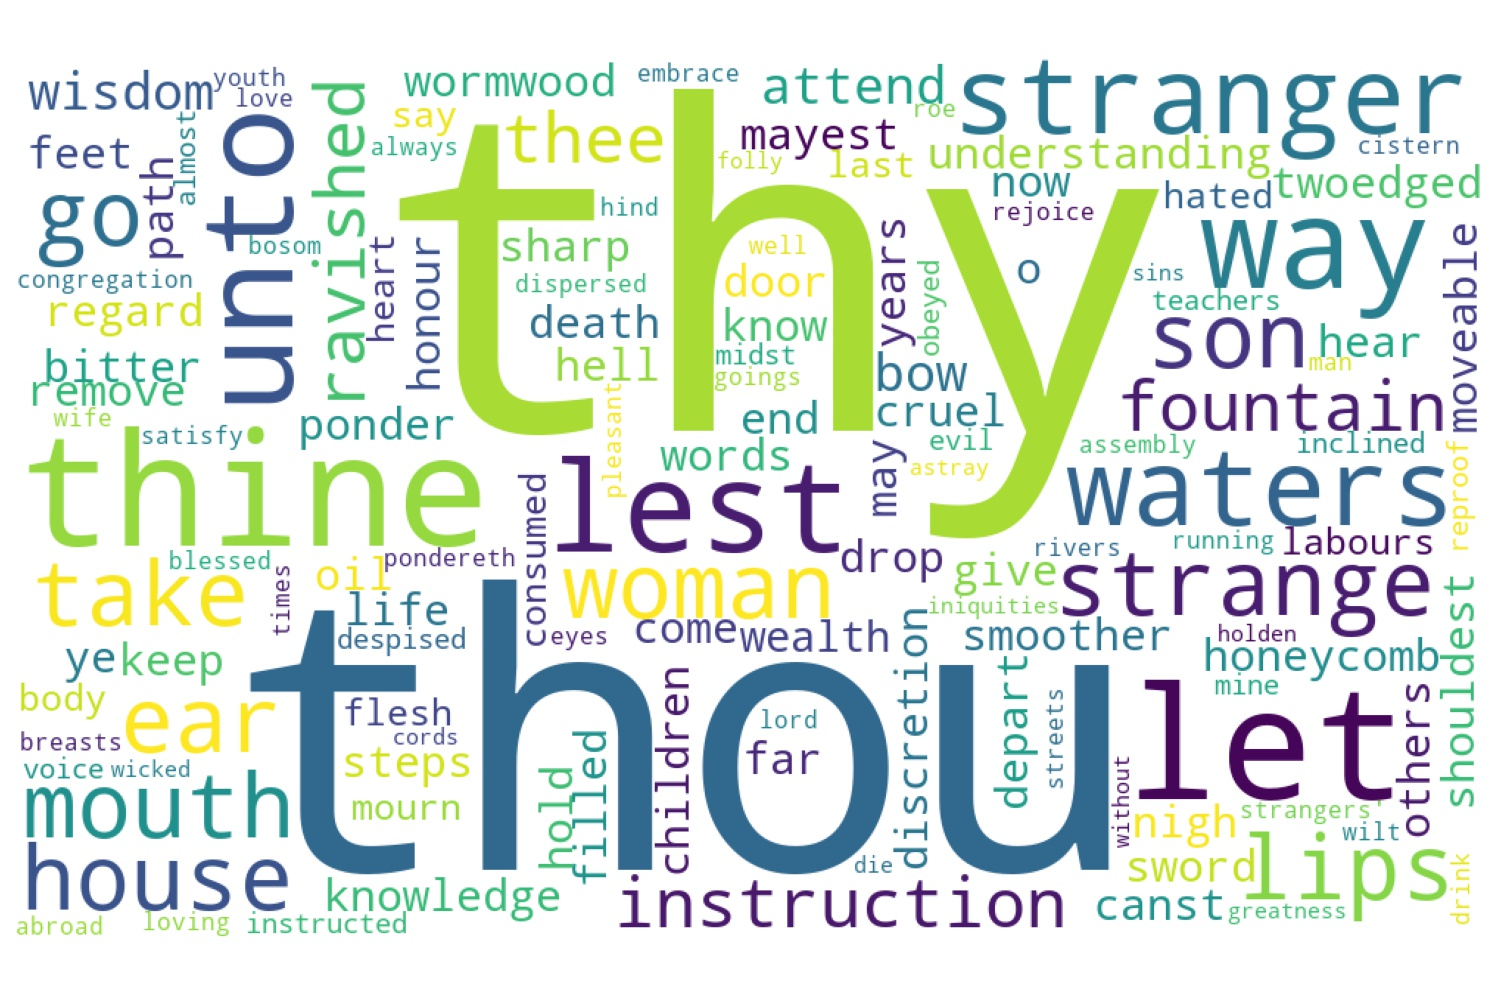
\includegraphics[width=\linewidth]{20OT-Proverbs/Proverb5-WordCloud.jpg}
  \caption{Proverb 5 Word Cloud}
  \label{fig:Proverb 5 Word Cloud}
\end{figure}

\marginpar{\scriptsize \centering \fcolorbox{bone}{lime}{\textbf{REGRETS}}\\ (Proverb 5:3-13) \begin{compactenum}[I.][8]
    \item  \textbf{Chased the Honeycomb!} \index[scripture]{Proverbs!Pro 05:03}(Pro 5:3)
    \item  \textbf{Wasted His Health} \index[scripture]{Proverbs!Pro 05:11}(Pro 5:11)
    \item  \textbf{Gave Away his Honor} \index[scripture]{Proverbs!Pro 05:09}(Pro 5:9)
    \item \textbf{Hated Instruction} \index[scripture]{Proverbs!Pro 05:12}(Pro 5:12)
    \item Did Not \textbf{Heed Correction} \index[scripture]{Proverbs!Pro 05:12}(Pro 5:12)
    \item Did Not \textbf{Harken Unto Teachers} \index[scripture]{Proverbs!Pro 05:13}(Pro 5:13)
    \item Did Not \textbf{Hear His Instructors} \index[scripture]{Proverbs!Pro 05:13}(Pro 5:13)
\end{compactenum}}

\marginpar{\scriptsize \centering \fcolorbox{bone}{yellow}{\textbf{THINE OWN CISTERN}}\\ (Proverb 5:25-21) \begin{compactenum}[I.][8]
    \item \textbf{Running Waters} \index[scripture]{Proverbs!Pro 05:15}(Pro 5:15)
    \item The \textbf{Reserving} \index[scripture]{Proverbs!Pro 05:17}(Pro 5:17)
    \item The \textbf{Rejoicing} \index[scripture]{Proverbs!Pro 05:18}(Pro 5:18)
    \item The \textbf{Roe} \index[scripture]{Proverbs!Pro 05:19}(Pro 5:19)
    \item The \textbf{Ravished} \index[scripture]{Proverbs!Pro 05:19}\index[scripture]{Proverbs!Pro 05:20}(Pro 5:19, 20)
    \item A \textbf{Rejection} \index[scripture]{Proverbs!Pro 05:20}(Pro 5:20)
    \item A \textbf{Review} \index[scripture]{Proverbs!Pro 05:21}(Pro 5:21)
\end{compactenum}}

\marginpar{\scriptsize \centering \fcolorbox{bone}{black}{\textbf{\textcolor[cmyk]{0,0,0,0}{STAY PURE \& ENJOY IT}}}\\ (Proverb 5) 
\begin{compactenum}[I.][8]
    \item The \textbf{Father's Appeal} \index[scripture]{Proverbs!Pro 05:01} \index[scripture]{Proverbs!Pro 05:07} (Pro 5:1, 7)
    \item The \textbf{Fleshly Appetite} 
    \item The \textbf{Fatal Attraction}   \index[scripture]{Proverbs!Pro 05:03-05}  (Pro 5:3-5)
    \item The \textbf{Foolish Absurdity}   \index[scripture]{Proverbs!Pro 05:21}  (Pro 5:21)
    \item The \textbf{Faithful Attention}  
    \item The \textbf{Fruitful Arrangement}   \index[scripture]{Proverbs!Pro 05:15-19}  (Pro 5:15-19)
    \item The \textbf{Final Accountability}   \index[scripture]{Proverbs!Pro 05:21}  (Pro 5:21)
\end{compactenum}}

\marginpar{\scriptsize \centering \fcolorbox{bone}{blue}{\textbf{\textcolor[cmyk]{0,0,0,0}{SEE THE SEDUCTRESS}}}\\ (Proverbs 5) 
\begin{compactenum}[I.][8]
    \item She has lips of honey \index[scripture]{Proverbs!Pro 05:03} (Pro 5:3) 
    \item She has a mouth smooth as oil \index[scripture]{Proverbs!Pro 05:03} (Pro 5:3)
    \item Her end is as bitter wormwood \index[scripture]{Proverbs!Pro 05:04} (Pro  5:4)
    \item Her feet walk the road to ruin \index[scripture]{Proverbs!Pro 05:05} (Pro 5:5)
    \item Her steps (direction) are to death \index[scripture]{Proverbs!Pro 05:05} (Pro 5:5)
\end{compactenum}}

\footnote{\textcolor[cmyk]{0.99998,1,0,0}{\hyperlink{TOC}{Return to end of Table of Contents.}}}\footnote{\href{https://audiobible.com/bible/proverbs_5.html}{\textcolor[cmyk]{0.99998,1,0,0}{Proverbs Audio}}}\textcolor[cmyk]{0.99998,1,0,0}{My son, attend unto my wisdom, \emph{and} bow thine ear to my \fcolorbox{bone}{MYGOLD}{understanding}:}
[2] \textcolor[cmyk]{0.99998,1,0,0}{That thou mayest regard discretion, and \emph{that} thy lips may keep knowledge.}\\
\\
\P \textcolor[cmyk]{0.99998,1,0,0}{For the lips of a strange woman drop \emph{as} an \fcolorbox{bone}{lime}{honeycomb}, and her mouth \emph{is} smoother than oil:}\footnote{\textbf{Hebrews 4:12} - For the word of God is quick, and powerful, and sharper than any twoedged sword, piercing even to the dividing asunder of soul and spirit, and of the joints and marrow, and is a discerner of the thoughts and intents of the heart.}
[4] \textcolor[cmyk]{0.99998,1,0,0}{But her end is bitter as wormwood, sharp as a twoedged sword.}
[5] \textcolor[cmyk]{0.99998,1,0,0}{Her feet go down to death; her steps take hold on hell.}
[6] \textcolor[cmyk]{0.99998,1,0,0}{Lest thou shouldest ponder the path of life, her ways are moveable, \emph{that} thou canst not know \emph{them}.}\footnote{\textbf{Psalm 16:11} - Thou wilt shew me the path of life: in thy presence is fulness of joy; at thy right hand there are pleasures for evermore.}\footnote{\textbf{Psalm 27:11} - Teach me thy way, O LORD, and lead me in a plain path, because of mine enemies.}\footnote{\textbf{Psalm 139:3} - Thou compassest my path and my lying down, and art acquainted with all my ways.}\footnote{\textbf{Psalm 142:3} - When my spirit was overwhelmed within me, then thou knewest my path. In the way wherein I walked have they privily laid a snare for me.}
[7] \textcolor[cmyk]{0.99998,1,0,0}{Hear me now therefore, O ye children, and depart not from the words of my mouth.}
[8] \textcolor[cmyk]{0.99998,1,0,0}{Remove thy way far from her, and come not nigh the door of her house:}
[9] \textcolor[cmyk]{0.99998,1,0,0}{Lest thou give thine honour unto others, and thy years unto the cruel:}
[10] \textcolor[cmyk]{0.99998,1,0,0}{Lest strangers be filled with thy wealth; and thy labours \emph{be} in the house of a stranger;}
[11] \textcolor[cmyk]{0.99998,1,0,0}{And thou mourn at the last, when thy \fcolorbox{bone}{lime}{flesh and thy body are consumed},}
[12] \textcolor[cmyk]{0.99998,1,0,0}{And say, How have I \fcolorbox{bone}{lime}{hated instruction}, and my heart \fcolorbox{bone}{lime}{despised reproof};}
[13] \textcolor[cmyk]{0.99998,1,0,0}{And have not obeyed \fcolorbox{bone}{lime}{the voice of my teachers}, nor \fcolorbox{bone}{lime}{inclined mine ear} to them that instructed me!}
[14] \textcolor[cmyk]{0.99998,1,0,0}{I was almost in all evil in the midst of the congregation and assembly.}\\
\\
\P \textcolor[cmyk]{0.99998,1,0,0}{Drink waters out of thine own cistern, and running waters out of thine own well.}\footnote{\textbf{2 Kings 18:31} - Hearken not to Hezekiah: for thus saith the king of Assyria, Make an agreement with me by a present, and come out to me, and then eat ye every man of his own vine, and every one of his fig tree, and drink ye every one the waters of his cistern:}\footnote{\textbf{Isaiah 36:16} - Hearken not to Hezekiah: for thus saith the king of Assyria, Make an agreement with me by a present, and come out to me: and eat ye every one of his vine, and every one of his fig tree, and drink ye every one the waters of his own cistern;}
[16] \textcolor[cmyk]{0.99998,1,0,0}{Let thy fountains be dispersed abroad, \emph{and} rivers of waters in the streets.}\footnote{\textbf{Psalm 127:4-5} - As arrows are in the hand of a mighty man; so are children of the youth. [5] Happy is the man that hath his quiver full of them: they shall not be ashamed, but they shall speak with the enemies in the gate.}
[17] \textcolor[cmyk]{0.99998,1,0,0}{Let them be only thine own, and not strangers' with thee.}
[18] \textcolor[cmyk]{0.99998,1,0,0}{Let thy fountain be blessed: and rejoice with the wife of thy youth.}
[19] \textcolor[cmyk]{0.99998,1,0,0}{\emph{Let} \emph{her} \emph{be} \emph{as} the loving hind and pleasant roe; let her breasts satisfy thee at all times; and be thou ravished always with her love.}
[20] \textcolor[cmyk]{0.99998,1,0,0}{And why wilt thou, my son, be ravished with a strange woman, and embrace the bosom of a stranger?}
[21] \textcolor[cmyk]{0.99998,1,0,0}{For the ways of man \emph{are} before the eyes of the LORD, and he pondereth all his goings.}\\
\\
\P \textcolor[cmyk]{0.99998,1,0,0}{His own iniquities shall take the wicked himself, and he shall be holden with the cords of his sins.}
[23] \textcolor[cmyk]{0.99998,1,0,0}{He shall die without instruction; and in the greatness of his folly he shall go astray.}





\index[NWIV]{13!Proverbs!Pro 05:001}\index[AWIP]{My!Proverbs!Pro 05:001}\index[AWIP]{son!Proverbs!Pro 05:001}\index[AWIP]{attend!Proverbs!Pro 05:001}\index[AWIP]{unto!Proverbs!Pro 05:001}\index[AWIP]{my!Proverbs!Pro 05:001}\index[AWIP]{wisdom!Proverbs!Pro 05:001}\index[AWIP]{\emph{and}!Proverbs!Pro 05:001}\index[AWIP]{bow!Proverbs!Pro 05:001}\index[AWIP]{thine!Proverbs!Pro 05:001}\index[AWIP]{ear!Proverbs!Pro 05:001}\index[AWIP]{to!Proverbs!Pro 05:001}\index[AWIP]{my!Proverbs!Pro 05:001 (2)}\index[AWIP]{understanding!Proverbs!Pro 05:001}

\index[DOCTRINES]{Practicology - wisdom!Proverbs!Pro 05:001}
\index[DOCTRINES]{Practicology - understanding!Proverbs!Pro 05:001}

\index[NWIV]{12!Proverbs!Pro 05:002}\index[AWIP]{That!Proverbs!Pro 05:002}\index[AWIP]{thou!Proverbs!Pro 05:002}\index[AWIP]{mayest!Proverbs!Pro 05:002}\index[AWIP]{regard!Proverbs!Pro 05:002}\index[AWIP]{discretion!Proverbs!Pro 05:002}\index[AWIP]{and!Proverbs!Pro 05:002}\index[AWIP]{\emph{that}!Proverbs!Pro 05:002}\index[AWIP]{thy!Proverbs!Pro 05:002}\index[AWIP]{lips!Proverbs!Pro 05:002}\index[AWIP]{may!Proverbs!Pro 05:002}\index[AWIP]{keep!Proverbs!Pro 05:002}\index[AWIP]{knowledge!Proverbs!Pro 05:002}

\index[DOCTRINES]{Practicology - wisdom!Proverbs!Pro 05:002}
\index[DOCTRINES]{Practicology - discretion!Proverbs!Pro 05:002}
\index[DOCTRINES]{Practicology - speech!Proverbs!Pro 05:002}

\index[NWIV]{18!Proverbs!Pro 05:003}\index[AWIP]{For!Proverbs!Pro 05:003}\index[AWIP]{the!Proverbs!Pro 05:003}\index[AWIP]{lips!Proverbs!Pro 05:003}\index[AWIP]{of!Proverbs!Pro 05:003}\index[AWIP]{a!Proverbs!Pro 05:003}\index[AWIP]{strange!Proverbs!Pro 05:003}\index[AWIP]{woman!Proverbs!Pro 05:003}\index[AWIP]{drop!Proverbs!Pro 05:003}\index[AWIP]{\emph{as}!Proverbs!Pro 05:003}\index[AWIP]{an!Proverbs!Pro 05:003}\index[AWIP]{honeycomb!Proverbs!Pro 05:003}\index[AWIP]{and!Proverbs!Pro 05:003}\index[AWIP]{her!Proverbs!Pro 05:003}\index[AWIP]{mouth!Proverbs!Pro 05:003}\index[AWIP]{\emph{is}!Proverbs!Pro 05:003}\index[AWIP]{smoother!Proverbs!Pro 05:003}\index[AWIP]{than!Proverbs!Pro 05:003}\index[AWIP]{oil!Proverbs!Pro 05:003}

\index[DOCTRINES]{Strange woman - lips as a honeycomb!Proverbs!Pro 05:003}
\index[DOCTRINES]{Strange woman - mouth smoother than oil!Proverbs!Pro 05:003}
\index[DOCTRINES]{Practicology - speech!Proverbs!Pro 05:003}

\index[NWIV]{12!Proverbs!Pro 05:004}\index[AWIP]{But!Proverbs!Pro 05:004}\index[AWIP]{her!Proverbs!Pro 05:004}\index[AWIP]{end!Proverbs!Pro 05:004}\index[AWIP]{is!Proverbs!Pro 05:004}\index[AWIP]{bitter!Proverbs!Pro 05:004}\index[AWIP]{as!Proverbs!Pro 05:004}\index[AWIP]{wormwood!Proverbs!Pro 05:004}\index[AWIP]{sharp!Proverbs!Pro 05:004}\index[AWIP]{as!Proverbs!Pro 05:004 (2)}\index[AWIP]{a!Proverbs!Pro 05:004}\index[AWIP]{twoedged!Proverbs!Pro 05:004}\index[AWIP]{sword!Proverbs!Pro 05:004}\index[DOCTRINES]{Sin -  False Religion (personified as a woman)!Proverbs!Pro 05:004}

\index[NWIV]{12!Proverbs!Pro 05:005}\index[AWIP]{Her!Proverbs!Pro 05:005}\index[AWIP]{feet!Proverbs!Pro 05:005}\index[AWIP]{go!Proverbs!Pro 05:005}\index[AWIP]{down!Proverbs!Pro 05:005}\index[AWIP]{to!Proverbs!Pro 05:005}\index[AWIP]{death!Proverbs!Pro 05:005}\index[AWIP]{her!Proverbs!Pro 05:005}\index[AWIP]{steps!Proverbs!Pro 05:005}\index[AWIP]{take!Proverbs!Pro 05:005}\index[AWIP]{hold!Proverbs!Pro 05:005}\index[AWIP]{on!Proverbs!Pro 05:005}\index[AWIP]{hell!Proverbs!Pro 05:005}\index[DOCTRINES]{Sin -  False Religion (personified as a woman)!Proverbs!Pro 05:005}

\index[NWIV]{18!Proverbs!Pro 05:006}\index[AWIP]{Lest!Proverbs!Pro 05:006}\index[AWIP]{thou!Proverbs!Pro 05:006}\index[AWIP]{shouldest!Proverbs!Pro 05:006}\index[AWIP]{ponder!Proverbs!Pro 05:006}\index[AWIP]{the!Proverbs!Pro 05:006}\index[AWIP]{path!Proverbs!Pro 05:006}\index[AWIP]{of!Proverbs!Pro 05:006}\index[AWIP]{life!Proverbs!Pro 05:006}\index[AWIP]{her!Proverbs!Pro 05:006}\index[AWIP]{ways!Proverbs!Pro 05:006}\index[AWIP]{are!Proverbs!Pro 05:006}\index[AWIP]{moveable!Proverbs!Pro 05:006}\index[AWIP]{\emph{that}!Proverbs!Pro 05:006}\index[AWIP]{thou!Proverbs!Pro 05:006 (2)}\index[AWIP]{canst!Proverbs!Pro 05:006}\index[AWIP]{not!Proverbs!Pro 05:006}\index[AWIP]{know!Proverbs!Pro 05:006}\index[AWIP]{\emph{them}!Proverbs!Pro 05:006}\index[DOCTRINES]{Sin -  False Religion (personified as a woman)!Proverbs!Pro 05:006}

\index[NWIV]{16!Proverbs!Pro 05:007}\index[AWIP]{Hear!Proverbs!Pro 05:007}\index[AWIP]{me!Proverbs!Pro 05:007}\index[AWIP]{now!Proverbs!Pro 05:007}\index[AWIP]{therefore!Proverbs!Pro 05:007}\index[AWIP]{O!Proverbs!Pro 05:007}\index[AWIP]{ye!Proverbs!Pro 05:007}\index[AWIP]{children!Proverbs!Pro 05:007}\index[AWIP]{and!Proverbs!Pro 05:007}\index[AWIP]{depart!Proverbs!Pro 05:007}\index[AWIP]{not!Proverbs!Pro 05:007}\index[AWIP]{from!Proverbs!Pro 05:007}\index[AWIP]{the!Proverbs!Pro 05:007}\index[AWIP]{words!Proverbs!Pro 05:007}\index[AWIP]{of!Proverbs!Pro 05:007}\index[AWIP]{my!Proverbs!Pro 05:007}\index[AWIP]{mouth!Proverbs!Pro 05:007}

\index[NWIV]{15!Proverbs!Pro 05:008}\index[AWIP]{Remove!Proverbs!Pro 05:008}\index[AWIP]{thy!Proverbs!Pro 05:008}\index[AWIP]{way!Proverbs!Pro 05:008}\index[AWIP]{far!Proverbs!Pro 05:008}\index[AWIP]{from!Proverbs!Pro 05:008}\index[AWIP]{her!Proverbs!Pro 05:008}\index[AWIP]{and!Proverbs!Pro 05:008}\index[AWIP]{come!Proverbs!Pro 05:008}\index[AWIP]{not!Proverbs!Pro 05:008}\index[AWIP]{nigh!Proverbs!Pro 05:008}\index[AWIP]{the!Proverbs!Pro 05:008}\index[AWIP]{door!Proverbs!Pro 05:008}\index[AWIP]{of!Proverbs!Pro 05:008}\index[AWIP]{her!Proverbs!Pro 05:008 (2)}\index[AWIP]{house!Proverbs!Pro 05:008}\index[DOCTRINES]{Sin -  False Religion (personified as a woman)!Proverbs!Pro 05:008}

\index[NWIV]{13!Proverbs!Pro 05:009}\index[AWIP]{Lest!Proverbs!Pro 05:009}\index[AWIP]{thou!Proverbs!Pro 05:009}\index[AWIP]{give!Proverbs!Pro 05:009}\index[AWIP]{thine!Proverbs!Pro 05:009}\index[AWIP]{honour!Proverbs!Pro 05:009}\index[AWIP]{unto!Proverbs!Pro 05:009}\index[AWIP]{others!Proverbs!Pro 05:009}\index[AWIP]{and!Proverbs!Pro 05:009}\index[AWIP]{thy!Proverbs!Pro 05:009}\index[AWIP]{years!Proverbs!Pro 05:009}\index[AWIP]{unto!Proverbs!Pro 05:009 (2)}\index[AWIP]{the!Proverbs!Pro 05:009}\index[AWIP]{cruel!Proverbs!Pro 05:009}

\index[DOCTRINES]{Sin - regret!Proverbs!Pro 05:009}

\index[NWIV]{17!Proverbs!Pro 05:010}\index[AWIP]{Lest!Proverbs!Pro 05:010}\index[AWIP]{strangers!Proverbs!Pro 05:010}\index[AWIP]{be!Proverbs!Pro 05:010}\index[AWIP]{filled!Proverbs!Pro 05:010}\index[AWIP]{with!Proverbs!Pro 05:010}\index[AWIP]{thy!Proverbs!Pro 05:010}\index[AWIP]{wealth!Proverbs!Pro 05:010}\index[AWIP]{and!Proverbs!Pro 05:010}\index[AWIP]{thy!Proverbs!Pro 05:010 (2)}\index[AWIP]{labours!Proverbs!Pro 05:010}\index[AWIP]{\emph{be}!Proverbs!Pro 05:010}\index[AWIP]{in!Proverbs!Pro 05:010}\index[AWIP]{the!Proverbs!Pro 05:010}\index[AWIP]{house!Proverbs!Pro 05:010}\index[AWIP]{of!Proverbs!Pro 05:010}\index[AWIP]{a!Proverbs!Pro 05:010}\index[AWIP]{stranger!Proverbs!Pro 05:010}

\index[DOCTRINES]{Sin - regret!Proverbs!Pro 05:010}

\index[NWIV]{14!Proverbs!Pro 05:011}\index[AWIP]{And!Proverbs!Pro 05:011}\index[AWIP]{thou!Proverbs!Pro 05:011}\index[AWIP]{mourn!Proverbs!Pro 05:011}\index[AWIP]{at!Proverbs!Pro 05:011}\index[AWIP]{the!Proverbs!Pro 05:011}\index[AWIP]{last!Proverbs!Pro 05:011}\index[AWIP]{when!Proverbs!Pro 05:011}\index[AWIP]{thy!Proverbs!Pro 05:011}\index[AWIP]{flesh!Proverbs!Pro 05:011}\index[AWIP]{and!Proverbs!Pro 05:011}\index[AWIP]{thy!Proverbs!Pro 05:011 (2)}\index[AWIP]{body!Proverbs!Pro 05:011}\index[AWIP]{are!Proverbs!Pro 05:011}\index[AWIP]{consumed!Proverbs!Pro 05:011}

\index[DOCTRINES]{Sin - regret!Proverbs!Pro 05:011}

\index[NWIV]{12!Proverbs!Pro 05:012}\index[AWIP]{And!Proverbs!Pro 05:012}\index[AWIP]{say!Proverbs!Pro 05:012}\index[AWIP]{How!Proverbs!Pro 05:012}\index[AWIP]{have!Proverbs!Pro 05:012}\index[AWIP]{I!Proverbs!Pro 05:012}\index[AWIP]{hated!Proverbs!Pro 05:012}\index[AWIP]{instruction!Proverbs!Pro 05:012}\index[AWIP]{and!Proverbs!Pro 05:012}\index[AWIP]{my!Proverbs!Pro 05:012}\index[AWIP]{heart!Proverbs!Pro 05:012}\index[AWIP]{despised!Proverbs!Pro 05:012}\index[AWIP]{reproof!Proverbs!Pro 05:012}\index[PNIP]{I!Proverbs!Pro 05:012}

\index[NWIV]{18!Proverbs!Pro 05:013}\index[AWIP]{And!Proverbs!Pro 05:013}\index[AWIP]{have!Proverbs!Pro 05:013}\index[AWIP]{not!Proverbs!Pro 05:013}\index[AWIP]{obeyed!Proverbs!Pro 05:013}\index[AWIP]{the!Proverbs!Pro 05:013}\index[AWIP]{voice!Proverbs!Pro 05:013}\index[AWIP]{of!Proverbs!Pro 05:013}\index[AWIP]{my!Proverbs!Pro 05:013}\index[AWIP]{teachers!Proverbs!Pro 05:013}\index[AWIP]{nor!Proverbs!Pro 05:013}\index[AWIP]{inclined!Proverbs!Pro 05:013}\index[AWIP]{mine!Proverbs!Pro 05:013}\index[AWIP]{ear!Proverbs!Pro 05:013}\index[AWIP]{to!Proverbs!Pro 05:013}\index[AWIP]{them!Proverbs!Pro 05:013}\index[AWIP]{that!Proverbs!Pro 05:013}\index[AWIP]{instructed!Proverbs!Pro 05:013}\index[AWIP]{me!Proverbs!Pro 05:013}


\index[NWIV]{14!Proverbs!Pro 05:014}\index[AWIP]{I!Proverbs!Pro 05:014}\index[AWIP]{was!Proverbs!Pro 05:014}\index[AWIP]{almost!Proverbs!Pro 05:014}\index[AWIP]{in!Proverbs!Pro 05:014}\index[AWIP]{all!Proverbs!Pro 05:014}\index[AWIP]{evil!Proverbs!Pro 05:014}\index[AWIP]{in!Proverbs!Pro 05:014 (2)}\index[AWIP]{the!Proverbs!Pro 05:014}\index[AWIP]{midst!Proverbs!Pro 05:014}\index[AWIP]{of!Proverbs!Pro 05:014}\index[AWIP]{the!Proverbs!Pro 05:014 (2)}\index[AWIP]{congregation!Proverbs!Pro 05:014}\index[AWIP]{and!Proverbs!Pro 05:014}\index[AWIP]{assembly!Proverbs!Pro 05:014}\index[PNIP]{I!Proverbs!Pro 05:014}
\index[DOCTRINES]{Practicology - rescued!Proverbs!Pro 05:014}

\index[NWIV]{15!Proverbs!Pro 05:015}\index[AWIP]{Drink!Proverbs!Pro 05:015}\index[AWIP]{waters!Proverbs!Pro 05:015}\index[AWIP]{out!Proverbs!Pro 05:015}\index[AWIP]{of!Proverbs!Pro 05:015}\index[AWIP]{thine!Proverbs!Pro 05:015}\index[AWIP]{own!Proverbs!Pro 05:015}\index[AWIP]{cistern!Proverbs!Pro 05:015}\index[AWIP]{and!Proverbs!Pro 05:015}\index[AWIP]{running!Proverbs!Pro 05:015}\index[AWIP]{waters!Proverbs!Pro 05:015 (2)}\index[AWIP]{out!Proverbs!Pro 05:015 (2)}\index[AWIP]{of!Proverbs!Pro 05:015 (2)}\index[AWIP]{thine!Proverbs!Pro 05:015 (2)}\index[AWIP]{own!Proverbs!Pro 05:015 (2)}\index[AWIP]{well!Proverbs!Pro 05:015}

\index[NWIV]{13!Proverbs!Pro 05:016}\index[AWIP]{Let!Proverbs!Pro 05:016}\index[AWIP]{thy!Proverbs!Pro 05:016}\index[AWIP]{fountains!Proverbs!Pro 05:016}\index[AWIP]{be!Proverbs!Pro 05:016}\index[AWIP]{dispersed!Proverbs!Pro 05:016}\index[AWIP]{abroad!Proverbs!Pro 05:016}\index[AWIP]{\emph{and}!Proverbs!Pro 05:016}\index[AWIP]{rivers!Proverbs!Pro 05:016}\index[AWIP]{of!Proverbs!Pro 05:016}\index[AWIP]{waters!Proverbs!Pro 05:016}\index[AWIP]{in!Proverbs!Pro 05:016}\index[AWIP]{the!Proverbs!Pro 05:016}\index[AWIP]{streets!Proverbs!Pro 05:016}

\index[NWIV]{11!Proverbs!Pro 05:017}\index[AWIP]{Let!Proverbs!Pro 05:017}\index[AWIP]{them!Proverbs!Pro 05:017}\index[AWIP]{be!Proverbs!Pro 05:017}\index[AWIP]{only!Proverbs!Pro 05:017}\index[AWIP]{thine!Proverbs!Pro 05:017}\index[AWIP]{own!Proverbs!Pro 05:017}\index[AWIP]{and!Proverbs!Pro 05:017}\index[AWIP]{not!Proverbs!Pro 05:017}\index[AWIP]{strangers'!Proverbs!Pro 05:017}\index[AWIP]{with!Proverbs!Pro 05:017}\index[AWIP]{thee!Proverbs!Pro 05:017}

\index[NWIV]{13!Proverbs!Pro 05:018}\index[AWIP]{Let!Proverbs!Pro 05:018}\index[AWIP]{thy!Proverbs!Pro 05:018}\index[AWIP]{fountain!Proverbs!Pro 05:018}\index[AWIP]{be!Proverbs!Pro 05:018}\index[AWIP]{blessed!Proverbs!Pro 05:018}\index[AWIP]{and!Proverbs!Pro 05:018}\index[AWIP]{rejoice!Proverbs!Pro 05:018}\index[AWIP]{with!Proverbs!Pro 05:018}\index[AWIP]{the!Proverbs!Pro 05:018}\index[AWIP]{wife!Proverbs!Pro 05:018}\index[AWIP]{of!Proverbs!Pro 05:018}\index[AWIP]{thy!Proverbs!Pro 05:018 (2)}\index[AWIP]{youth!Proverbs!Pro 05:018}

\index[NWIV]{26!Proverbs!Pro 05:019}\index[AWIP]{\emph{Let}!Proverbs!Pro 05:019}\index[AWIP]{\emph{her}!Proverbs!Pro 05:019}\index[AWIP]{\emph{be}!Proverbs!Pro 05:019}\index[AWIP]{\emph{as}!Proverbs!Pro 05:019}\index[AWIP]{the!Proverbs!Pro 05:019}\index[AWIP]{loving!Proverbs!Pro 05:019}\index[AWIP]{hind!Proverbs!Pro 05:019}\index[AWIP]{and!Proverbs!Pro 05:019}\index[AWIP]{pleasant!Proverbs!Pro 05:019}\index[AWIP]{roe!Proverbs!Pro 05:019}\index[AWIP]{let!Proverbs!Pro 05:019}\index[AWIP]{her!Proverbs!Pro 05:019}\index[AWIP]{breasts!Proverbs!Pro 05:019}\index[AWIP]{satisfy!Proverbs!Pro 05:019}\index[AWIP]{thee!Proverbs!Pro 05:019}\index[AWIP]{at!Proverbs!Pro 05:019}\index[AWIP]{all!Proverbs!Pro 05:019}\index[AWIP]{times!Proverbs!Pro 05:019}\index[AWIP]{and!Proverbs!Pro 05:019 (2)}\index[AWIP]{be!Proverbs!Pro 05:019}\index[AWIP]{thou!Proverbs!Pro 05:019}\index[AWIP]{ravished!Proverbs!Pro 05:019}\index[AWIP]{always!Proverbs!Pro 05:019}\index[AWIP]{with!Proverbs!Pro 05:019}\index[AWIP]{her!Proverbs!Pro 05:019 (2)}\index[AWIP]{love!Proverbs!Pro 05:019}

\index[NWIV]{19!Proverbs!Pro 05:020}\index[AWIP]{And!Proverbs!Pro 05:020}\index[AWIP]{why!Proverbs!Pro 05:020}\index[AWIP]{wilt!Proverbs!Pro 05:020}\index[AWIP]{thou!Proverbs!Pro 05:020}\index[AWIP]{my!Proverbs!Pro 05:020}\index[AWIP]{son!Proverbs!Pro 05:020}\index[AWIP]{be!Proverbs!Pro 05:020}\index[AWIP]{ravished!Proverbs!Pro 05:020}\index[AWIP]{with!Proverbs!Pro 05:020}\index[AWIP]{a!Proverbs!Pro 05:020}\index[AWIP]{strange!Proverbs!Pro 05:020}\index[AWIP]{woman!Proverbs!Pro 05:020}\index[AWIP]{and!Proverbs!Pro 05:020}\index[AWIP]{embrace!Proverbs!Pro 05:020}\index[AWIP]{the!Proverbs!Pro 05:020}\index[AWIP]{bosom!Proverbs!Pro 05:020}\index[AWIP]{of!Proverbs!Pro 05:020}\index[AWIP]{a!Proverbs!Pro 05:020 (2)}\index[AWIP]{stranger!Proverbs!Pro 05:020}
\index[DOCTRINES]{Sin -  False Religion (personified as a woman)!Proverbs!Pro 05:020}


\index[NWIV]{18!Proverbs!Pro 05:021}\index[AWIP]{For!Proverbs!Pro 05:021}\index[AWIP]{the!Proverbs!Pro 05:021}\index[AWIP]{ways!Proverbs!Pro 05:021}\index[AWIP]{of!Proverbs!Pro 05:021}\index[AWIP]{man!Proverbs!Pro 05:021}\index[AWIP]{\emph{are}!Proverbs!Pro 05:021}\index[AWIP]{before!Proverbs!Pro 05:021}\index[AWIP]{the!Proverbs!Pro 05:021 (2)}\index[AWIP]{eyes!Proverbs!Pro 05:021}\index[AWIP]{of!Proverbs!Pro 05:021 (2)}\index[AWIP]{the!Proverbs!Pro 05:021 (3)}\index[AWIP]{LORD!Proverbs!Pro 05:021}\index[AWIP]{and!Proverbs!Pro 05:021}\index[AWIP]{he!Proverbs!Pro 05:021}\index[AWIP]{pondereth!Proverbs!Pro 05:021}\index[AWIP]{all!Proverbs!Pro 05:021}\index[AWIP]{his!Proverbs!Pro 05:021}\index[AWIP]{goings!Proverbs!Pro 05:021}\index[PNIP]{LORD!Proverbs!Pro 05:021}

\index[NWIV]{19!Proverbs!Pro 05:022}\index[AWIP]{His!Proverbs!Pro 05:022}\index[AWIP]{own!Proverbs!Pro 05:022}\index[AWIP]{iniquities!Proverbs!Pro 05:022}\index[AWIP]{shall!Proverbs!Pro 05:022}\index[AWIP]{take!Proverbs!Pro 05:022}\index[AWIP]{the!Proverbs!Pro 05:022}\index[AWIP]{wicked!Proverbs!Pro 05:022}\index[AWIP]{himself!Proverbs!Pro 05:022}\index[AWIP]{and!Proverbs!Pro 05:022}\index[AWIP]{he!Proverbs!Pro 05:022}\index[AWIP]{shall!Proverbs!Pro 05:022 (2)}\index[AWIP]{be!Proverbs!Pro 05:022}\index[AWIP]{holden!Proverbs!Pro 05:022}\index[AWIP]{with!Proverbs!Pro 05:022}\index[AWIP]{the!Proverbs!Pro 05:022 (2)}\index[AWIP]{cords!Proverbs!Pro 05:022}\index[AWIP]{of!Proverbs!Pro 05:022}\index[AWIP]{his!Proverbs!Pro 05:022}\index[AWIP]{sins!Proverbs!Pro 05:022}

\index[NWIV]{16!Proverbs!Pro 05:023}\index[AWIP]{He!Proverbs!Pro 05:023}\index[AWIP]{shall!Proverbs!Pro 05:023}\index[AWIP]{die!Proverbs!Pro 05:023}\index[AWIP]{without!Proverbs!Pro 05:023}\index[AWIP]{instruction!Proverbs!Pro 05:023}\index[AWIP]{and!Proverbs!Pro 05:023}\index[AWIP]{in!Proverbs!Pro 05:023}\index[AWIP]{the!Proverbs!Pro 05:023}\index[AWIP]{greatness!Proverbs!Pro 05:023}\index[AWIP]{of!Proverbs!Pro 05:023}\index[AWIP]{his!Proverbs!Pro 05:023}\index[AWIP]{folly!Proverbs!Pro 05:023}\index[AWIP]{he!Proverbs!Pro 05:023}\index[AWIP]{shall!Proverbs!Pro 05:023 (2)}\index[AWIP]{go!Proverbs!Pro 05:023}\index[AWIP]{astray!Proverbs!Pro 05:023}


%%%%%%%%%%%%%%%%%%%%%%%%%%%
%%%%%%%%%%%%%%%%%%%%%%%%%%%

\index[DOCTRINES]{Sin - destiny!Proverbs!Pro 05:023}
\index[DOCTRINES]{Sin - folly!Proverbs!Pro 05:023}

\index[DOCTRINES]{Practicology - seeking!Proverbs!Pro 05:012}
\index[DOCTRINES]{Practicology - seeking!Proverbs!Pro 05:013}
\index[DOCTRINES]{Practicology - seeking!Proverbs!Pro 05:023}

\index[DOCTRINES]{Unregenerate Living - personified as a woman!Proverbs!Pro 05:022}
\index[DOCTRINES]{Strange woman - ravishes!Proverbs!Pro 05:020}
\index[DOCTRINES]{Sin - regret!Proverbs!Pro 05:013}



\index[DOCTRINES]{Sin - regret!Proverbs!Pro 05:012}
\index[DOCTRINES]{Practicology - heart!Proverbs!Pro 05:012}



\section{Proverb 5 Outlines}

\subsection{My Outlines}

\subsubsection{Regrets of a Sensual Son}
\textbf{Introduction: }In Proverb 5 we see what the sensual son regrets he did not do. He wishes he had:
\index[speaker]{Keith Anthony!Proverb 05 (Regrets of a Sensual Son)}
\index[series]{Proverbs (Keith Anthony)!Pro 05 (Regrets of a Sensual Son)}
\index[date]{2014/12/06!Proverb 05 (Regrets of a Sensual Son) (Keith Anthony)}
\begin{compactenum}[I.][8]

    \item  \textbf{Chased the Honeycomb!} \index[scripture]{Proverbs!Pro 05:03} (Pro 5:3)
    \item  \textbf{Wasted His Health} \index[scripture]{Proverbs!Pro 05:11} (Pro 5:11)
    \item  \textbf{Gave Away his Honor} \index[scripture]{Proverbs!Pro 05:09} (Pro 5:9)
    \item \textbf{Hated Instruction} \index[scripture]{Proverbs!Pro 05:12} (Pro 5:12)
    \item Did Not \textbf{Heed Correction} \index[scripture]{Proverbs!Pro 05:12} (Pro 5:12)
    \item Did Not \textbf{Harken Unto Teachers} \index[scripture]{Proverbs!Pro 05:13} (Pro 5:13)
    \item Did Not \textbf{Hear His Instructors} \index[scripture]{Proverbs!Pro 05:13} ( Pro 5:13)
    
\end{compactenum}


\subsubsection{Thine Own Cistern}

\index[speaker]{Keith Anthony!Proverb 05 (Thine Own Cistern)}
\index[series]{Proverbs (Keith Anthony)!Pro 05 (Thine Own Cistern)}
\index[date]{2014/12/06!Proverb 05 (Thine Own Cistern) (Keith Anthony)}

\begin{compactenum}[I.][8]
    \item \textbf{Running Waters} \index[scripture]{Proverbs!Pro 05:15}(Pro 5:15)
    \item The \textbf{Reserving} \index[scripture]{Proverbs!Pro 05:17}(Pro 5:17)
    \item The \textbf{Rejoicing} \index[scripture]{Proverbs!Pro 05:18}(Pro 5:18)
    \item The \textbf{Roe} \index[scripture]{Proverbs!Pro 05:19}(Pro 5:19)
    \item The \textbf{Ravished} \index[scripture]{Proverbs!Pro 05:19}\index[scripture]{Proverbs!Pro 05:20}(Pro 5:19, 20)
    \item A \textbf{Rejection} \index[scripture]{Proverbs!Pro 05:20}(Pro 5:20)
    \item A \textbf{Review} \index[scripture]{Proverbs!Pro 05:21}(Pro 5:21)
\end{compactenum}





\subsubsection{Stay Pure and Enjoy it}
\textbf{Introduction:} Proverbs 5 is entirely devoted to the subject of sexual and marital Proverbs 5 contains essential wisdom on pre-marital and extra-marital sexual relations:
\index[speaker]{Keith Anthony!Proverb 05 (Stay Pure and Enjoy it)}
\index[series]{Proverbs (Keith Anthony)!Pro 05 (Stay Pure and Enjoy it)}
\index[date]{unknown!Proverb 05 (Stay Pure and Enjoy it) (Keith Anthony)}

\begin{compactenum}[I.]
    \item \textbf{The Father's Appeal} \index[scripture]{Proverbs!Pro 05:01,07}(Proverbs 5:1, 7) There are two separate appeals in the proverb, in verses 1 and 7.  Some divide the chapter into three sections: verses 1-6, verses 7-14, and verses 15-23. The first two contain the father's emotional appeal.
    \item \textbf{A Fleshly Appetite} The appetite for sexual relations is built into mankind.  It exists.  It is natural. It is even wholesome when directed according to God's will. As with all things, though, Satan provides counterfeit and convenient ways to get side-tracked.
    \item \textbf{A Fatal Attraction} \index[scripture]{Proverbs!Pro 05:03-05}(Pro 5:3-5) Consider the death spiral of verses 3-5.
    \item \textbf{A Foolish Absurdity} - It is foolish and absurd to think that marital infidelity can be done is secret or with impunity. \index[scripture]{Proverbs!Pro 05:21}(Pro 5:21) reminds that the ``eyes of the Lord'' are watching, and seemingly watching especially this!
    \item \textbf{Faithful Attention} The challenge is given to the son to stay faithful to only the one God has provided, and to garner immense satisfaction from the relationship. The challenge is given to want, to be ravished by, what you already have, and not to want something else.
    \item \textbf{A Fruitful Arrangement} \index[scripture]{Proverbs!Pro 05:15-19}(Pro 5:15-19) In verses 15 and 16, the author uses the metaphor of a flowing waters (cisterns, wells, foundations, rivers). In verse 17, attention is brought to the unique privilege of marriage. In verses 18 and 19, a request is made to bless the wife in the context of marital relations.
    \item \textbf{Final Accountability} \index[scripture]{Proverbs!Pro 05:21}(Pro 5:21) The passage, finally, and teachers of it should also, reminds us that God will hold all accountable for behavior, including sexual behavior. In the temporal experience, even modern   medicine, psychology, and sociology confirm that promiscuity is self-destructive.
\end{compactenum}

\subsubsection{See the Seductress}
\textbf{Introduction:} Proverb 5 is entirely devoted to the subject of sexual and marital purity. The chapter contains 4 verses with 13 words, with 4 being the number for creation (all 4 directions on a compass) and 13 the number of rebellion. The number 5, the chapter address, is also the number of death, suggesting the serious of the issue.  Verses 3-5 even have a 5-fold description of the the strange woman:
\index[speaker]{Keith Anthony!Proverb 05 (See the Seductress)}
\index[series]{Proverbs (Keith Anthony)!Pro 05 (See the Seductress)}
\index[date]{unknown!Proverb 05 (See the Seductress) (Keith Anthony)}
\begin{compactenum}[I.]
    \item She has lips of honey \index[scripture]{Proverbs!Pro 05:03} (Pro 5:3) 
    \item She has a mouth smooth as oil \index[scripture]{Proverbs!Pro 05:03} ( Pro 5:3)
    \item Her end is as bitter wormwood \index[scripture]{Proverbs!Pro 05:04} (Pro  5:4)
    \item Her feet walk the road to ruin \index[scripture]{Proverbs!Pro 05:05} (Pro 5:5)
    \item Her steps (direction) are to death \index[scripture]{Proverbs!Pro 05:05} Pro 5:5)
\end{compactenum}
\textbf{Conclusion:} Chapter 5, though, also contains God's wonderful solution to the problem of mankind's promiscuity. This suggests that the problem discussed in the chapter is a very common and natural (to a natural lost man and lost culture) thing.  Adultery assuredly is a common problem even among Christian marriages. Pre-marital relationships are trap which often keeps one for life. Proverbs 5 does not deal with the issue delicately: it deals with the issue directly.  There are sexual urges and appetites that exist and which must be controlled and directly the correct way.  Otherwise, it will be misery and ruin.
\subsection{Outlines from Others}

\section{Proverb 5 Comments}

\subsection{Numeric Nuggets}
\textbf{13:} In the chapter, verses 1, 9, 16, and 18 have 13 words. The chapter uses the 13-letter word ``understanding.'' The word ``understanding'' is the 13$^{th}$ word in the chapter! Verses 11, and 6  have 13 unique words. There are 13 words in italics in the chapter.

%\subsection{Proverb 5:3}
%\subsection{Proverb 5:4}
%\subsection{Proverb 5:5}
%\subsection{Proverb 5:6}
%\subsection{Proverb 5:7}
%\subsection{Proverb 5:8}
%\subsection{Proverb 5:9}
%\subsection{Proverb 5:10} 

\subsection{Proverb 5:16}
\begin{center}

\begin{table}[ht]
\centering
\begin{tabular}{|p{.5in}|p{3.5in}|}
    \hline

\textcolor[rgb]{0.00,0.00,1.00}{AV} & \textcolor[rgb]{0.00,0.00,1.00}{Let thy fountains be dispersed abroad, and rivers of waters in the streets.} \\ \hline

ASV &  Should thy springs be dispersed abroad, And streams of water in the streets?\\ \hline

CEB &  Should your fountains flood outside, streams of water in the public squares?\\ \hline

ESV & Should your springs be scattered abroad, streams of water in the streets? \\ \hline

NASV & Should your springs overflow into the street, Streams of water in the public squares\\ \hline

MEV & Should your fountains be dispersed abroad, streams of water in the streets?\\ \hline

NIV &  Should your springs overflow in the streets, your streams of water in the public squares? \\ \hline

NKJV & Should your fountains be dispersed abroad, Streams of water in the streets?.\\ \hline

RSV & Should your springs be scattered abroad, streams of water in the streets?\\ \hline

 \multicolumn{2}{p{4.3in}}{{Following the word ``not'' which was inserted by Origen into the verse. The result changes a command into a question. Where did we see that first? The conspiracy results from a misunderstanding of ``well'' in verse 15, and ``fountains'' in verse 16. The word ``well'' refers to the wife, and ``fountains'' to children. The admonition is (1) to have children with your own wife, while not allowing other men to do so, and (2) have children and send them out (like arrows in a quiver - Psalm 127:4). The singular ``fountain,'' in verse 18, is the wife.}} \\
\end{tabular}
 
\caption[Corruption Alert: Proverb 5:16]{Corruption Alert: Proverb 5:16} \label{table:Corruption Proverb 5:16}
\end{table}

\end{center}




\subsection{Proverb 5:19}
See references to breasts in Song of Solomon (verses 1:13, 4:5, 7:3, 7:7, 7:8, 8:1, 8:8, and 8:10). 

\subsection{Proverb 5:20}
Why indeed? Warnings against such have been provided, the right way prepared. 

\subsection{Proverb 5:21}
One of the things being pondered, no doubt, is the question posed in verse 20. See references to the ``eyes of the Lord'', found 22 times, in 21 chapters, in 13 books (Genesis 6:8, Deuteronomy 11:12, Deuteronomy 13:18, 1 Samuel 26:24, 2 Samuel 15:25, 1 Kings 15:5, 1 Kings 15:11, 1 Kings 16:25, 1 Kings 22:43, 2 Chronicles 14:2, 2 Chronicles 16:9, 2 Chronicles 21:6, 2 Chronicles 29:6, Psalms 34:15, Proverbs 5:21, Proverbs 15:3, Proverbs 22:12, Isaiah 49:5, Jeremiah 52:2, Amos 9:8, Zechariah 4:10, and 1 Peter 3:12).


\subsection{Proverb  5 Repeated Phrases}


%%%%%%%%%%
%%%%%%%%%%
\normalsize
 
\begin{center}
\begin{longtable}{|p{3.0in}|p{0.5in}|}
\caption[Proverb  5 Repeated Phrases]{Proverb  5 Repeated Phrases}\label{table:Repeated Phrases Proverb  5} \\
\hline \multicolumn{1}{|c|}{\textbf{Phrase}} & \multicolumn{1}{c|}{\textbf{Frequency}} \\ \hline 
\endfirsthead
 
\multicolumn{2}{c}
{{\bfseries \tablename\ \thetable{} -- continued from previous page}} \\  
\hline \multicolumn{1}{|c|}{\textbf{Phrase}} & \multicolumn{1}{c|}{\textbf{Frequency}} \\ \hline 
\endhead
 
\hline \multicolumn{2}{c}{{ }} \\ \hline
\endfoot 
in the & 4\\ \hline 
of a & 3\\ \hline 
and thy & 3\\ \hline 
thine own & 3\\ \hline 
\end{longtable}
\end{center}



%%%%%%%%%%
%%%%%%%%%%



%\newpage
\section{Proverb 5 Statistics}

%%%%%%%%%%%%%%%%%%%%%%%%%%%
%%%%% Word Statistics
%%%%%%%%%%%%%%%%%%%%%%%%%%

\normalsize
\subsection{Chapter Word Statistics}


%%%%%%%%%%
%%%%%%%%%%
 
\begin{center}
\begin{longtable}{l|c|c|c|c}
\caption[Stats for Proverb 5]{Stats for Proverb 5} \label{table:Stats for Proverb 5} \\ 
\hline \multicolumn{1}{|c|}{\textbf{Verse(s)}} & \multicolumn{1}{|c|}{\textbf{Count}} & \multicolumn{1}{|c|}{\textbf{Unique}} & \multicolumn{1}{|c|}{\textbf{Italics}} & \multicolumn{1}{|c|}{\textbf{Uniq Italic}}  \\ \hline 
\endfirsthead
 
\multicolumn{5}{c}
{{\bfseries \tablename\ \thetable{} -- continued from previous page}} \\  
\hline \multicolumn{1}{|c|}{\textbf{Verse(s)}} & \multicolumn{1}{|c|}{\textbf{Count}} & \multicolumn{1}{|c|}{\textbf{Unique}} & \multicolumn{1}{|c|}{\textbf{Italics}} & \multicolumn{1}{|c|}{\textbf{Uniq Italic}}  \\ \hline 
\endhead
 
\hline \multicolumn{5}{|r|}{{Continued if needed}} \\ \hline
\endfoot 
1 & 13 & 12 & 1 & 1\\ \hline
2 & 12 & 12 & 1 & 1\\ \hline
3 & 18 & 18 & 2 & 2\\ \hline
4 & 12 & 11 & 0 & 0\\ \hline
5 & 12 & 12 & 0 & 0\\ \hline
6 & 18 & 17 & 2 & 2\\ \hline
7 & 16 & 16 & 0 & 0\\ \hline
8 & 15 & 14 & 0 & 0\\ \hline
9 & 13 & 12 & 0 & 0\\ \hline
10 & 17 & 16 & 1 & 1\\ \hline
11 & 14 & 13 & 0 & 0\\ \hline
12 & 12 & 12 & 0 & 0\\ \hline
13 & 18 & 18 & 0 & 0\\ \hline
14 & 14 & 12 & 0 & 0\\ \hline
15 & 15 & 10 & 0 & 0\\ \hline
16 & 13 & 13 & 1 & 1\\ \hline
17 & 11 & 11 & 0 & 0\\ \hline
18 & 13 & 12 & 0 & 0\\ \hline
19 & 26 & 24 & 4 & 4\\ \hline
20 & 19 & 18 & 0 & 0\\ \hline
21 & 18 & 15 & 1 & 1\\ \hline
22 & 19 & 17 & 0 & 0\\ \hline
23 & 16 & 15 & 0 & 0\\ \hline
\hline \hline
Total & 354 & 196 & 13 & 9




\end{longtable}
\end{center}

%%%%%%%%%%
%%%%%%%%%%


\subsection{Words by Frequency}

\begin{center}
\begin{longtable}{l|r}
\caption[Word Frequencies in Proverb 5]{Word Frequencies in Proverb 5} \label{table:WordsIn-Proverb-5} \\ 
\hline \multicolumn{1}{|c|}{\textbf{Word}} & \multicolumn{1}{c|}{\textbf{Frequency}} \\ \hline 
\endfirsthead
  
\multicolumn{2}{c}  
{{\bfseries \tablename\ \thetable{} -- continued from previous page}} \\   
\hline \multicolumn{1}{|c|}{\textbf{Word}} & \multicolumn{1}{c|}{\textbf{Frequency}} \\ \hline   
\endhead  
  
\hline \multicolumn{2}{|r|}{{Continue}} \\ \hline  
\endfoot  
  
\hline \hline  
\endlastfoot  
  
the & 20\\ \hline 
and & 18\\ \hline 
of & 16\\ \hline 
thy & 10\\ \hline 
her & 8\\ \hline 
thou & 7\\ \hline 
be & 7\\ \hline 
my & 6\\ \hline 
with & 6\\ \hline 
thine & 5\\ \hline 
a & 5\\ \hline 
not & 5\\ \hline 
in & 5\\ \hline 
And & 4\\ \hline 
own & 4\\ \hline 
shall & 4\\ \hline 
unto & 3\\ \hline 
to & 3\\ \hline 
Lest & 3\\ \hline 
all & 3\\ \hline 
waters & 3\\ \hline 
Let & 3\\ \hline 
he & 3\\ \hline 
his & 3\\ \hline 
son & 2\\ \hline 
\emph{and} & 2\\ \hline 
ear & 2\\ \hline 
\emph{that} & 2\\ \hline 
lips & 2\\ \hline 
For & 2\\ \hline 
strange & 2\\ \hline 
woman & 2\\ \hline 
\emph{as} & 2\\ \hline 
mouth & 2\\ \hline 
as & 2\\ \hline 
go & 2\\ \hline 
take & 2\\ \hline 
ways & 2\\ \hline 
are & 2\\ \hline 
me & 2\\ \hline 
from & 2\\ \hline 
house & 2\\ \hline 
\emph{be} & 2\\ \hline 
stranger & 2\\ \hline 
at & 2\\ \hline 
have & 2\\ \hline 
I & 2\\ \hline 
instruction & 2\\ \hline 
them & 2\\ \hline 
out & 2\\ \hline 
thee & 2\\ \hline 
ravished & 2\\ \hline 
My & 1\\ \hline 
attend & 1\\ \hline 
wisdom & 1\\ \hline 
bow & 1\\ \hline 
understanding & 1\\ \hline 
That & 1\\ \hline 
mayest & 1\\ \hline 
regard & 1\\ \hline 
discretion & 1\\ \hline 
may & 1\\ \hline 
keep & 1\\ \hline 
knowledge & 1\\ \hline 
drop & 1\\ \hline 
an & 1\\ \hline 
honeycomb & 1\\ \hline 
\emph{is} & 1\\ \hline 
smoother & 1\\ \hline 
than & 1\\ \hline 
oil & 1\\ \hline 
But & 1\\ \hline 
end & 1\\ \hline 
is & 1\\ \hline 
bitter & 1\\ \hline 
wormwood & 1\\ \hline 
sharp & 1\\ \hline 
twoedged & 1\\ \hline 
sword & 1\\ \hline 
Her & 1\\ \hline 
feet & 1\\ \hline 
down & 1\\ \hline 
death & 1\\ \hline 
steps & 1\\ \hline 
hold & 1\\ \hline 
on & 1\\ \hline 
hell & 1\\ \hline 
shouldest & 1\\ \hline 
ponder & 1\\ \hline 
path & 1\\ \hline 
life & 1\\ \hline 
moveable & 1\\ \hline 
canst & 1\\ \hline 
know & 1\\ \hline 
\emph{them} & 1\\ \hline 
Hear & 1\\ \hline 
now & 1\\ \hline 
therefore & 1\\ \hline 
O & 1\\ \hline 
ye & 1\\ \hline 
children & 1\\ \hline 
depart & 1\\ \hline 
words & 1\\ \hline 
Remove & 1\\ \hline 
way & 1\\ \hline 
far & 1\\ \hline 
come & 1\\ \hline 
nigh & 1\\ \hline 
door & 1\\ \hline 
give & 1\\ \hline 
honour & 1\\ \hline 
others & 1\\ \hline 
years & 1\\ \hline 
cruel & 1\\ \hline 
strangers & 1\\ \hline 
filled & 1\\ \hline 
wealth & 1\\ \hline 
labours & 1\\ \hline 
mourn & 1\\ \hline 
last & 1\\ \hline 
when & 1\\ \hline 
flesh & 1\\ \hline 
body & 1\\ \hline 
consumed & 1\\ \hline 
say & 1\\ \hline 
How & 1\\ \hline 
hated & 1\\ \hline 
heart & 1\\ \hline 
despised & 1\\ \hline 
reproof & 1\\ \hline 
obeyed & 1\\ \hline 
voice & 1\\ \hline 
teachers & 1\\ \hline 
nor & 1\\ \hline 
inclined & 1\\ \hline 
mine & 1\\ \hline 
that & 1\\ \hline 
instructed & 1\\ \hline 
was & 1\\ \hline 
almost & 1\\ \hline 
evil & 1\\ \hline 
midst & 1\\ \hline 
congregation & 1\\ \hline 
assembly & 1\\ \hline 
Drink & 1\\ \hline 
cistern & 1\\ \hline 
running & 1\\ \hline 
well & 1\\ \hline 
fountains & 1\\ \hline 
dispersed & 1\\ \hline 
abroad & 1\\ \hline 
rivers & 1\\ \hline 
streets & 1\\ \hline 
only & 1\\ \hline 
strangers' & 1\\ \hline 
fountain & 1\\ \hline 
blessed & 1\\ \hline 
rejoice & 1\\ \hline 
wife & 1\\ \hline 
youth & 1\\ \hline 
\emph{Let} & 1\\ \hline 
\emph{her} & 1\\ \hline 
loving & 1\\ \hline 
hind & 1\\ \hline 
pleasant & 1\\ \hline 
roe & 1\\ \hline 
let & 1\\ \hline 
breasts & 1\\ \hline 
satisfy & 1\\ \hline 
times & 1\\ \hline 
always & 1\\ \hline 
love & 1\\ \hline 
why & 1\\ \hline 
wilt & 1\\ \hline 
embrace & 1\\ \hline 
bosom & 1\\ \hline 
man & 1\\ \hline 
\emph{are} & 1\\ \hline 
before & 1\\ \hline 
eyes & 1\\ \hline 
LORD & 1\\ \hline 
pondereth & 1\\ \hline 
goings & 1\\ \hline 
His & 1\\ \hline 
iniquities & 1\\ \hline 
wicked & 1\\ \hline 
himself & 1\\ \hline 
holden & 1\\ \hline 
cords & 1\\ \hline 
sins & 1\\ \hline 
He & 1\\ \hline 
die & 1\\ \hline 
without & 1\\ \hline 
greatness & 1\\ \hline 
folly & 1\\ \hline 
astray & 1\\ \hline 
\end{longtable}  
\end{center}  


  
\normalsize  

  
  


\subsection{Words Alphabetically}

\begin{center}
\begin{longtable}{l|r}
\caption[Word Frequencies in Proverb 5]{Word Frequencies in Proverb 5} \label{table:WordsIn-Proverb-5} \\ 
\hline \multicolumn{1}{|c|}{\textbf{Word}} & \multicolumn{1}{c|}{\textbf{Frequency}} \\ \hline 
\endfirsthead
  
\multicolumn{2}{c}  
{{\bfseries \tablename\ \thetable{} -- continued from previous page}} \\   
\hline \multicolumn{1}{|c|}{\textbf{Word}} & \multicolumn{1}{c|}{\textbf{Frequency}} \\ \hline   
\endhead  
  
\hline \multicolumn{2}{|r|}{{Continue}} \\ \hline  
\endfoot  
  
\hline \hline  
\endlastfoot  
  
And & 4\\ \hline 
But & 1\\ \hline 
Drink & 1\\ \hline 
For & 2\\ \hline 
He & 1\\ \hline 
Hear & 1\\ \hline 
Her & 1\\ \hline 
His & 1\\ \hline 
How & 1\\ \hline 
I & 2\\ \hline 
LORD & 1\\ \hline 
Lest & 3\\ \hline 
Let & 3\\ \hline 
My & 1\\ \hline 
O & 1\\ \hline 
Remove & 1\\ \hline 
That & 1\\ \hline 
\emph{Let} & 1\\ \hline 
\emph{and} & 2\\ \hline 
\emph{are} & 1\\ \hline 
\emph{as} & 2\\ \hline 
\emph{be} & 2\\ \hline 
\emph{her} & 1\\ \hline 
\emph{is} & 1\\ \hline 
\emph{that} & 2\\ \hline 
\emph{them} & 1\\ \hline 
a & 5\\ \hline 
abroad & 1\\ \hline 
all & 3\\ \hline 
almost & 1\\ \hline 
always & 1\\ \hline 
an & 1\\ \hline 
and & 18\\ \hline 
are & 2\\ \hline 
as & 2\\ \hline 
assembly & 1\\ \hline 
astray & 1\\ \hline 
at & 2\\ \hline 
attend & 1\\ \hline 
be & 7\\ \hline 
before & 1\\ \hline 
bitter & 1\\ \hline 
blessed & 1\\ \hline 
body & 1\\ \hline 
bosom & 1\\ \hline 
bow & 1\\ \hline 
breasts & 1\\ \hline 
canst & 1\\ \hline 
children & 1\\ \hline 
cistern & 1\\ \hline 
come & 1\\ \hline 
congregation & 1\\ \hline 
consumed & 1\\ \hline 
cords & 1\\ \hline 
cruel & 1\\ \hline 
death & 1\\ \hline 
depart & 1\\ \hline 
despised & 1\\ \hline 
die & 1\\ \hline 
discretion & 1\\ \hline 
dispersed & 1\\ \hline 
door & 1\\ \hline 
down & 1\\ \hline 
drop & 1\\ \hline 
ear & 2\\ \hline 
embrace & 1\\ \hline 
end & 1\\ \hline 
evil & 1\\ \hline 
eyes & 1\\ \hline 
far & 1\\ \hline 
feet & 1\\ \hline 
filled & 1\\ \hline 
flesh & 1\\ \hline 
folly & 1\\ \hline 
fountain & 1\\ \hline 
fountains & 1\\ \hline 
from & 2\\ \hline 
give & 1\\ \hline 
go & 2\\ \hline 
goings & 1\\ \hline 
greatness & 1\\ \hline 
hated & 1\\ \hline 
have & 2\\ \hline 
he & 3\\ \hline 
heart & 1\\ \hline 
hell & 1\\ \hline 
her & 8\\ \hline 
himself & 1\\ \hline 
hind & 1\\ \hline 
his & 3\\ \hline 
hold & 1\\ \hline 
holden & 1\\ \hline 
honeycomb & 1\\ \hline 
honour & 1\\ \hline 
house & 2\\ \hline 
in & 5\\ \hline 
inclined & 1\\ \hline 
iniquities & 1\\ \hline 
instructed & 1\\ \hline 
instruction & 2\\ \hline 
is & 1\\ \hline 
keep & 1\\ \hline 
know & 1\\ \hline 
knowledge & 1\\ \hline 
labours & 1\\ \hline 
last & 1\\ \hline 
let & 1\\ \hline 
life & 1\\ \hline 
lips & 2\\ \hline 
love & 1\\ \hline 
loving & 1\\ \hline 
man & 1\\ \hline 
may & 1\\ \hline 
mayest & 1\\ \hline 
me & 2\\ \hline 
midst & 1\\ \hline 
mine & 1\\ \hline 
mourn & 1\\ \hline 
mouth & 2\\ \hline 
moveable & 1\\ \hline 
my & 6\\ \hline 
nigh & 1\\ \hline 
nor & 1\\ \hline 
not & 5\\ \hline 
now & 1\\ \hline 
obeyed & 1\\ \hline 
of & 16\\ \hline 
oil & 1\\ \hline 
on & 1\\ \hline 
only & 1\\ \hline 
others & 1\\ \hline 
out & 2\\ \hline 
own & 4\\ \hline 
path & 1\\ \hline 
pleasant & 1\\ \hline 
ponder & 1\\ \hline 
pondereth & 1\\ \hline 
ravished & 2\\ \hline 
regard & 1\\ \hline 
rejoice & 1\\ \hline 
reproof & 1\\ \hline 
rivers & 1\\ \hline 
roe & 1\\ \hline 
running & 1\\ \hline 
satisfy & 1\\ \hline 
say & 1\\ \hline 
shall & 4\\ \hline 
sharp & 1\\ \hline 
shouldest & 1\\ \hline 
sins & 1\\ \hline 
smoother & 1\\ \hline 
son & 2\\ \hline 
steps & 1\\ \hline 
strange & 2\\ \hline 
stranger & 2\\ \hline 
strangers & 1\\ \hline 
strangers' & 1\\ \hline 
streets & 1\\ \hline 
sword & 1\\ \hline 
take & 2\\ \hline 
teachers & 1\\ \hline 
than & 1\\ \hline 
that & 1\\ \hline 
the & 20\\ \hline 
thee & 2\\ \hline 
them & 2\\ \hline 
therefore & 1\\ \hline 
thine & 5\\ \hline 
thou & 7\\ \hline 
thy & 10\\ \hline 
times & 1\\ \hline 
to & 3\\ \hline 
twoedged & 1\\ \hline 
understanding & 1\\ \hline 
unto & 3\\ \hline 
voice & 1\\ \hline 
was & 1\\ \hline 
waters & 3\\ \hline 
way & 1\\ \hline 
ways & 2\\ \hline 
wealth & 1\\ \hline 
well & 1\\ \hline 
when & 1\\ \hline 
why & 1\\ \hline 
wicked & 1\\ \hline 
wife & 1\\ \hline 
wilt & 1\\ \hline 
wisdom & 1\\ \hline 
with & 6\\ \hline 
without & 1\\ \hline 
woman & 2\\ \hline 
words & 1\\ \hline 
wormwood & 1\\ \hline 
ye & 1\\ \hline 
years & 1\\ \hline 
youth & 1\\ \hline 
\end{longtable}  
\end{center}  


  
\normalsize  

  
  
\subsection{Word Lengths in Chapter} 
\normalsize 
\begin{center} 
\begin{longtable}{l|p{3.75in}} 
\caption[Words by Length in Proverb 5]{Words by Length in Proverb 5} \label{table:WordsIn-Proverb-5} \\ 
\hline \multicolumn{1}{|c|}{\textbf{Length}} & \multicolumn{1}{c|}{\textbf{Words}} \\ \hline 
\endfirsthead 
 
\multicolumn{2}{c} 
{{\bfseries \tablename\ \thetable{} -- continued from previous page}} \\ 
\hline \multicolumn{1}{|c|}{\textbf{Length}} & \multicolumn{1}{c|}{\textbf{Words}} \\ \hline 
\endhead 
 
\hline \multicolumn{2}{|r|}{{Continued}} \\ \hline 
\endfoot 
 
\hline \hline 
\endlastfoot 
1 & a, O, I\\ \hline 
2 & My, my, to, of, \emph{as}, an, \emph{is}, is, as, go, on, me, ye, be, \emph{be}, in, at, he, He\\ \hline 
3 & son, \emph{and}, bow, ear, and, thy, may, For, the, her, oil, But, end, Her, are, not, now, way, far, And, say, How, nor, was, all, out, own, Let, \emph{Let}, \emph{her}, roe, let, why, man, \emph{are}, his, His, die\\ \hline 
4 & unto, That, thou, \emph{that}, lips, keep, drop, than, feet, down, take, hold, hell, Lest, path, life, ways, know, \emph{them}, Hear, from, come, nigh, door, give, with, last, when, body, have, mine, them, that, evil, well, only, thee, wife, hind, love, wilt, eyes, LORD, sins\\ \hline 
5 & thine, woman, mouth, sharp, sword, death, steps, canst, words, house, years, cruel, mourn, flesh, hated, heart, voice, midst, Drink, youth, times, bosom, shall, cords, folly\\ \hline 
6 & attend, wisdom, mayest, regard, bitter, ponder, depart, Remove, honour, others, filled, wealth, obeyed, almost, waters, abroad, rivers, loving, always, before, goings, wicked, holden, astray\\ \hline 
7 & strange, labours, reproof, cistern, running, streets, blessed, rejoice, breasts, satisfy, embrace, himself, without\\ \hline 
8 & smoother, wormwood, twoedged, moveable, children, stranger, consumed, despised, teachers, inclined, assembly, fountain, pleasant, ravished\\ \hline 
9 & knowledge, honeycomb, shouldest, therefore, strangers, fountains, dispersed, pondereth, greatness\\ \hline 
10 & discretion, instructed, strangers', iniquities\\ \hline 
11 & instruction\\ \hline 
12 & congregation\\ \hline 
13 & understanding\\ \hline 
\end{longtable} 
\end{center} 




%%%%%%%%%%
%%%%%%%%%%
 

%\input{20OT-Proverbs/Example-DEVOTIONAL-Psalm3-DEVOTIONAL-BryanChapel}


%%% For Indexes

%\index[DEVOTIONAL]{TGIF1!Os Hillman (Living for a Cause Greater Than Yourself) - Proverb 19:17!2021/12/21}

%\index[DEVOTIONAL]{TGIF1!Os Hillman (Living for a Cause Greater Than Yourself) - Proverb 19:17!2021/12/21}

















%%% colour: cardinal red - \textcolor[cmyk]{0,0.85,0.70,0.23}{text}


%%%% Example marginpar with a compactenum list --- green color text
%\marginpar{\scriptsize \textcolor[rgb]{0.00,0.545,0.269}{$\rightarrow$7 Abominations: 
%\begin{compactenum}
%	\item A proud look,
%	\item a lying tongue,
%	\item hands that shed innocent blood,
%	\item An heart that deviseth wicked imaginations,
%	\item feet that be swift in running to mischief,
%	\item A false witness that speaketh lies, and
%	\item he that soweth discord among brethren.
%\end{compactenum}}}



%\newpage

%\begin{mdframed}[style=MyFrame]
%\begin{center}
%\begin{longtable}{|p{.5in}|p{3.5in}|}

%\caption[Corruption Alert: Proverbs 18:1]{Corruption Alert: Proverbs 18:1} \label{table:CorruptionProv18:1} \\ 

%\hline  
%\multicolumn{1}{|c|}{\textbf{Version}} & 
%\multicolumn{1}{c|}{\textbf{Corruption}}  \\ \hline 
%\endfirsthead
 
%\multicolumn{2}{c}
%{{\bfseries \tablename\ \thetable{} -- continued from previous page}} \\  \hline  
%\multicolumn{1}{|c|}{\textbf{Version}} & 
%\multicolumn{1}{c|}{\textbf{Corruption}}  \\ \hline 
%\endhead
 
%\hline \multicolumn{2}{|r|}{{Continued on next page}} \\ \hline
%\endfoot 
%\textcolor[rgb]{0.00,0.00,1.00}{AV} & \textcolor[rgb]{0.00,0.00,1.00}{Through desire a man, having separated himself, seeketh \emph{and} intermeddleth with all wisdom.} \\ \hline
%
%ASV &  He that separateth himself seeketh his own desire, And  rageth against all sound wisdom. \\ \hline
%
%CEB &  Unfriendly people look out for themselves; they bicker with sensible people.\\ \hline
%
%ESV & Whoever isolates himself seeks his own desire;  he breaks out against all sound judgment. \\ \hline
%
%NASV &  He who separates himself seeks his own desire, He quarrels against all sound wisdom.\\ \hline
%
%MEV & He who separates himself seeks his own desire; he seeks and quarrels against all wisdom.\\ \hline
%
%NIV &  An unfriendly person pursues selfish ends and against all sound judgment starts quarrels. \\ \hline
%
%NKJV &  A man who isolates himself seeks his own desire; He rages against all wise judgment.\\ \hline
%
%RSV &  He who is estranged seeks pretexts  to break out against all sound judgment.\\ \hline

% \multicolumn{2}{p{4.3in}}{{Modern translations, such as the ASV and others, strike out the first part of the verse, concealing the intent of mankind in genewisdom clearly revealed in scripture. How wonderful is the obfuscated RSV text: ``He who is estranged seeks pretexts.'' What does THAT mean?}} \\ %\hline

%\hline

%\end{longtable}
%\end{center}

%\normalsize 
%\end{mdframed}

%\marginpar{\scriptsize \centering \fcolorbox{black}{lime}{\textbf{OUTIDE THE PLACE OF PROMISE}}\\ (Psalm 137:1--9) 
%\begin{compactenum}[I.][8]
%	\item \textbf{Plight \& Distress} \index[scripture]{Psalms!Psa 137:01} (Psalm 137:1)
%	\item The \textbf{Place Desired} \index[scripture]{Psalms!Psa 137:01} (Psalm 137:1)
%	\item \textbf{Pining \& Despiar} \index[scripture]{Psalms!Psa 137:02} (Psalm 137:2)
%	\item \textbf{Provoked \& Degraded}\index[scripture]{Psalms!Psa 137:03} (Psalm 137:3)
%	\item The \textbf{Predicament Described}\index[scripture]{Psalms!Psa 137:04} (Psalm 137:4)
%	\item A \textbf{Preference Decided}\index[scripture]{Psalms!Psa 137:06} (Psalm 137:6)
%	\item A \textbf{Prediction of Destruction}\index[scripture]{Psalms!Psa 137:08} (Psalm 137:8)
%\end{compactenum} }


%\subsection{Outlines from Others}

%\subsubsection{Words on Wisdom}
%\index[speaker]{John Battles!Proverbs 01 (Words on Wisdom)}
%\index[series]{Proverbs (John Battles)!Proverbs 01 (Words on Wisdom)}
%\index[date]{2016/01/20!Proverbs 01 (Words on Wisdom) (John Battles)}
%\textbf{Lineage}: adpated from S. Conway\\
%\textbf{Introduction}: Proverbs distinctly points out things that a fool does:
%\begin{compactenum}[I.][4]
%	\item \textbf{Welcome to Wisdom} \index[scripture]{Proverbs!Pro 01:01-09}(Proverbs 1:1-9)
%	\item \textbf{Warnings of Wisdom} \index[scripture]{Proverbs!Pro 01:10-19}(Proverbs 1:10-19).
%	\item \textbf{Woe of Wisdom} \index[scripture]{Proverbs!Pro 01:24-32}(Proverbs 1:24-32)
%	\item \textbf{Watchcare of Wisdom} \index[scripture]{Proverbs!Pro 01:33}(Proverbs 1:33).
%\end{compactenum}


%%%%% COLOR FOR MARGINPAR OUTLINES
%% 1  LIME - \marginpar{\scriptsize \centering \fcolorbox{black}{lime}{\textbf{TITLE}}\\ (Passage) 
%% 2. YELLOW - \marginpar{\scriptsize \centering \fcolorbox{black}{yellow}{\textbf{TITLE}}\\ (Passage) 
%% 3. Blue BGND, WHITE LETTERS - \marginpar{\scriptsize \centering \fcolorbox{black}{blue}{\textbf{\textcolor[cmyk]{0,0,0,0}{TITLE}}}\\ (Passage) 
%% 4. black BGND, WHITE LETTERS - \marginpar{\scriptsize \centering \fcolorbox{black}{black}{\textbf{\textcolor[cmyk]{0,0,0,0}{TITLE}}}\\ (Passage) 
%% 5. red BGND, WHITE LETTERS - \marginpar{\scriptsize \centering \fcolorbox{black}{red}{\textbf{\textcolor[cmyk]{0,0,0,0}{TITLE}}}\\ (Passage) 

%%%%%% INCLUSION OF GRAPHIC
%\newpage

%\begin{figure}
%\begin{center}
%\includegraphics[scale=0.5, angle=90]{07OT-Judges/References/b201107i1-large}
%\caption[Summary of the 13 Judges]{Summary of the 13 Judges}
%\label{fig:Summary of the 13 Judges}
%\end{center}
%\end{figure}


%%%%%%%%%%%
%%%%%%%%%%%

% SYTEMATIC THEOLOGY (10 + 2)
% Theology proper – The study of the character of God
% Angelology – The study of angels
% Biblical theology – The study of the Bible
% Christology – The study of Christ
% Ecclesiology – The study of the church
% Eschatology – The study of the end times[5]
% Hamartiology – The study of sin
% Pneumatology – The study of the Holy Spirit
% Soteriology – The study of salvation
% Theological anthropology – The study of the nature of humanity.
% ++
% Moral theology
% Bilical cosomolgy

%%%%%%%%%%%%%%
%%%%%%%%%%%%%%

% \footnote{\href{https://audiobible.com/bible/psalms_91.html}{\textcolor[cmyk]{0.99998,1,0,0}{Psalm 91 Audio}}}

% \marginpar{\scriptsize \centering \fcolorbox{black}{lime}{\textbf{JERUSALEM}}\\
% \fcolorbox{black}{lime}{\textbf{DON'T GO BACK TO EGYPT}} \\ (Isaiah 31:1--9) 

%%%%%%%%%%%%%%
%%% Extra Colors
%%% from https://latexcolor.blogspot.com/2019/10/list-of-latex-colors.html
%%%%%%%%%%%%%%
% \definecolor{champagne}{rgb}{0.97,0.91,0.81}
% \definecolor{bone}{rgb}{0.89,0.85,0.79}
%\titleJE
%

%%%%% EXAMPLE Index entry:
% \index[DOCTRINES]{Eschatology - Millennium!Psalms!Psa 069:036}

%%% for things found 13 times
%\fcolorbox{black}{bone}{TEXT}
\scriptsize

%%%%%%%%%%%%%%%%%%%%%%%%%%%%%
%Indices

\chapter{Indexes}
\printindex[DOCTRINES]
\printindex[scripture]
\printindex[speaker]
%\printindex[series]

\printindex[FACEBOOK]
\printindex[LOCATION]
\printindex[DEVOTIONAL]
\printindex[AWIP]

\printbibliography
\end{document}

